 \makeatletter
 {\def\thebibliography#1{\chapter*{\refname\@mkboth
 			{\uppercase{\refname}}{\uppercase{\refname}}}\list
 		{[\arabic{enumi}]}{\settowidth\labelwidth{[#1]}
 			\rightmargin\labelwidth
 			\advance\rightmargin\labelsep
 			\advance\rightmargin\bibindent
 			\itemindent -\bibindent
 			\listparindent \itemindent
 			\parsep \z@
 			\usecounter{enumi}}
 		\def\newblock{}
 		\sloppy
 		\sfcode`\.=1000\relax}}
 \makeatother
 \documentclass[a4paper,fleqn]{report} 
 %*************************************************
% All the packages and definitions required for this 
% project are included here.
%*************************************************
% Iman Izadi, 1394
% Dept. of Electrical and Computer Engineering, IUT
%*************************************************


\usepackage{amsthm,amssymb,amsmath}			% Writing math
\usepackage{epsf,graphicx}									% Including graphics
\usepackage[a4paper]{geometry}							% Fixing page layout and margins
\usepackage{titlesec}	
\usepackage{setspace}											% Change line spacing

\usepackage[stable,bottom]{footmisc}					% Move footnotes to the


\usepackage[pagebackref=false,colorlinks,linkcolor=blue,citecolor=red]{hyperref}
\usepackage{zref-perpage}
\usepackage{mathtools}
%\usepackage[demo]{graphicx}
\usepackage{caption}
%\usepackage{float}
	
\usepackage{colortbl,booktabs,tabularx}
\usepackage{subcaption}
\usepackage{adjustbox}
\usepackage[dvipsnames]{xcolor}


%\usepackage[backend=biber]{biblatex}
%\usepackage{zref-perpage}									% Reset footnote counter in each page
%\zmakeperpage[1]{footnote}

\usepackage{perpage}
\MakePerPage{footnote}

\usepackage{xepersian}										% Persian
\settextfont{XB Zar}	
											% Persian font
\definecolor{LightCyan}{rgb}{0,0.53,0.74}
%\addbibresource{reference.bib}

% Use English digits in equations
\DefaultMathsDigits

% Default footnotes from left to right
\setfootnoteLR

\setdigitfont[Scale=1]{XB Zar}
\setlatintextfont[Scale=1.2]{Times New Roman}

\DefaultMathsDigits

\makeatletter
\def\BState{\State\hskip-\ALG@thistlm}
\makeatother

% Use English digits in equations
%\DefaultMathsDigits

% Default footnotes from left to right
\setfootnoteLR

% Use English numbers for English footnotes
\makeatletter
\def\@makeLTRfnmark{\hbox{\@textsuperscript{\latinfont\@thefnmark}}}
\renewcommand\@makefntext[1]{%
	\parindent 1em%
	\noindent
	\hb@xt@1.8em{\hss\if@RTL\@makefnmark\else\@makeLTRfnmark\fi}#1}
\makeatother

% Use dash instead of dot in section numbers
\SepMark{-}										

% Change fonts and margins of section and subsection titles
% For chapters please see firstpages.tex
\titlespacing*{\section}{0pt}{1cm}{0.2cm}
\titleformat{\section}
{\fontsize{12}{6}\scshape\bfseries}{\thesection}{1em}{}

\titlespacing*{\subsection}{0pt}{.8cm}{0cm}
\titleformat{\subsection}
{\fontsize{11}{6}\scshape\bfseries}{\thesubsection}{1em}{}

% Fix table of contents for chapters
\makeatletter 
\def\@chapter[#1]#2{\ifnum \c@secnumdepth >\m@ne
	\refstepcounter{chapter}%
	\typeout{\@chapapp\space\thechapter.}%
	\addcontentsline{toc}{chapter}%
	{\@chapapp~\protect\numberline{\tartibi{chapter}\,:\space #1}}
	\else
	\addcontentsline{toc}{chapter}{#1}%
	\fi
	\chaptermark{#1}%
	\addtocontents{lof}{\protect\addvspace{10\p@}}%
	\addtocontents{lot}{\protect\addvspace{10\p@}}%
	\@makechapterhead{#2}%
	\@afterheading}
\makeatother


		
 \defpersianfont\titlefont[Scale=1]{XB Titre}
 \renewcommand{\bibname}{\rl{مراجع}}	
 
 \begin{document}
 	
	%*************************************************
% In this file the first few pages are typeset.
% Make changes accordingly.
%*************************************************
\pagenumbering{adadi}
%***************************
% Page 1: Blank
%***************************
\thispagestyle{empty}
\mbox{}
\pagebreak


%***************************
% Page 2: Besmelah
%***************************
%\setcounter{page}{5}
\thispagestyle{empty}
\begin{center}
	~\vfill
	
\includegraphics[scale=1]{firstpage-img/besm}
	~\vfill
\end{center}
\pagebreak

%***************************
% Page 3: Title
%***************************
\thispagestyle{empty}
\newgeometry{left=3cm,right=3cm,top=2cm}
\begin{center}
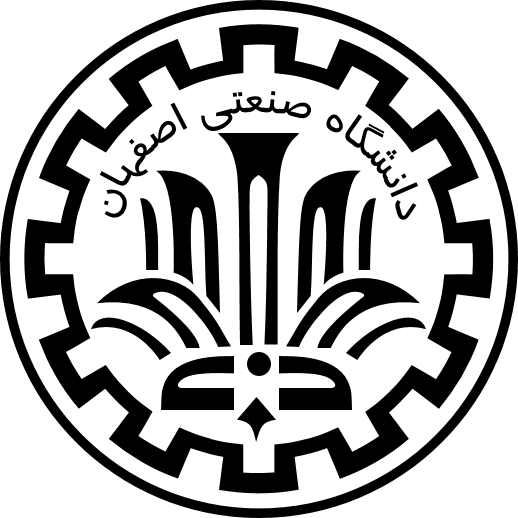
\includegraphics[height=3cm]{firstpage-img/iut_logo_fa}
%\vspace{0.5cm}

{\large
	\textbf{دانشگاه صنعتی اصفهان}\\
	دانشکده  برق و کامپیوتر
}
\vspace{3.5cm}

{\LARGE
	\textbf{توسعه‌ی ماشین بلتزمن محدود برای مدل‌سازی مشترک موضوع و احساس در داده‌های متنی}\\
}
\vspace{3.5cm}

{\large
	\textbf{پایان‌نامه کارشناسی ارشد مهندسی کامپیوتر - هوش مصنوعی}\\
}
\vspace{1cm}

{\Large
	\textbf{مسعود فاطمی}\\
}
\vspace{2.5cm}

{\large
	استاد راهنما\\
}
\vspace{0.5cm}

{\Large
	\textbf{دکتر مهران صفایانی}\\
}
\vspace{1cm}
{\large
	استاد مشاور\\
}
\vspace{0.5cm}
{\Large
	\textbf{دکتر عبدالرضا میرزایی}\\
}
\vspace{2cm}

{\Large
	\textbf{1395}
}

\end{center}
\restoregeometry
\pagebreak

%***************************
% page 4: Signatures
%***************************
\thispagestyle{empty}
\newgeometry{left=3cm,right=3cm,top=2cm}
\begin{center}
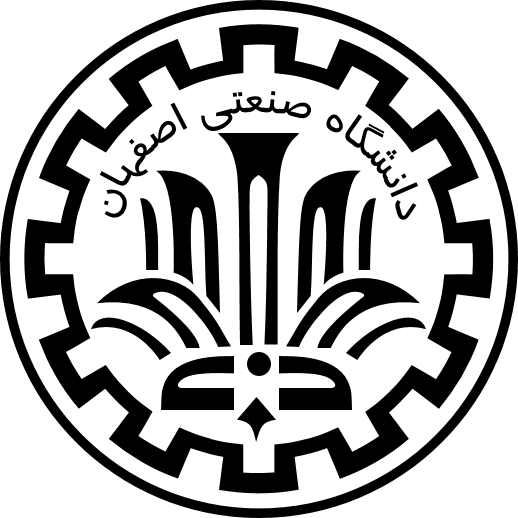
\includegraphics[height=3cm]{firstpage-img/iut_logo_fa}
%\vspace{0.5cm}

{\large
	\textbf{دانشگاه صنعتی اصفهان}\\
	دانشکده  برق و کامپیوتر
}
	%	\vspace{5cm}
	
	\vfill
	
	{\Large
		پایان‌نامه کارشناسی ارشد رشته مهندسی کامپیوتر -- هوش‌مصنوعی و رباتیک \\
		\vspace{.3cm}
		مسعود فاطمی\\
		\vspace{.3cm}
		تحت عنوان\\
	}
\end{center}

\begin{center}
	{\large
		\textbf{ توسعه‌ی ماشین بلتزمن محدود برای مدل‌سازی مشترک موضوع و احساس در داده‌های متنی}
	}
\end{center}
\vspace*{1.8cm}
در تاریخ ۹۶/۳/۲۷ توسط کمیته‌ی تخصصی زیر مورد بررسی و تصویب نهایی قرار گرفت:\\

{\normalsize
	
	\begin{tabular}{rr}
		\vspace*{.8cm}
		1- استاد راهنمای پایان‌نامه  & \hspace{2cm} دکتر مهران صفایانی \\
		\vspace{.8cm}
		۲- استاد مشاور پایان‌نامه &\hspace{2cm} دکتر عبدالرضا میرزایی \\
		\vspace{.8cm}
		۳-استاد داور  &\hspace{2cm}  دکتر محمدرضا احمدزاده\\
		\vspace{.8cm}
		۴-استاد داور (اختیاری) &\hspace{2cm}  دکتر مریم ذکری \\
		\vspace{.8cm}
		سرپرست تحصیلات تکمیلی دانشکده &\hspace{2cm} دکتر محمد رضا تابان \\
	\end{tabular}
}
\restoregeometry
\pagebreak



%***************************
% Page 5: Acknowledgment (Optional)
%***************************
\thispagestyle{empty}
\vspace*{3cm}
\settextfont{IranNastaliq}

{\large
	\textbf{تشکر و قدردانی}\\

	
پروردگار منّان را سپاسگزارم ......

}
\restoregeometry
\pagebreak
\settextfont{XB Zar}
%***************************
% page 6: Rights
%***************************
\thispagestyle{empty}
\newgeometry{left=6cm,right=6cm}

\begin{spacing}{3}
	\leavevmode
	\vfill
	\parbox{8 cm}{
		
		\textbf{\Large کلیه حقوق مادی مترتب بر نتایج مطالعات، ابتکارات و نوآوری‌های ناشی از تحقیق موضوع این پایان‌نامه متعلق به دانشگاه صنعتی اصفهان است.}
		
	}
	\vfill
\end{spacing}
\restoregeometry
\pagebreak

%***************************
% page 7: Dedication
%***************************
\thispagestyle{empty}
\newgeometry{left=4.5cm,right=4.5cm,top=5cm,bottom=5cm}


\settextfont{IranNastaliq}
\vspace*{\fill}
\begin{center}
{\LARGE تقدیم به}\\
\vspace{1cm}
\textbf{{\Huge پدر و مادرم}}
\end{center}
\vspace*{\fill}

\bgroup\vspace*{\fill}
\renewcommand{\\}{\vspace{-.5em}\newline\relax}
\newcommand{\تب}[1][.5]{\hspace*{#1cm}}
\noindent
\vspace*{\fill}\egroup
\pagebreak

\settextfont{XB Zar}
%***************************
% page 8-13: Table of contents
%***************************
\titleformat{\chapter}[display]
	{\normalfont\LARGE\bfseries\centering}{\chaptertitlename ~ \tartibi{chapter}}{20pt}{\LARGE}

\newgeometry{left=2.5cm,right=3cm,top=3cm,bottom=2.5cm,includehead=false,headsep=1cm,footnotesep=.5cm}
\baselineskip=.7cm

\addtocontents{toc}{\textbf{\underline{عنوان}}}
\addtocontents{toc}{\hfill\textbf{\underline{صفحه}}\par}
\tableofcontents
\listoffigures
\listoftables
\pagebreak

%***************************
% page 14: vocabulary
%***************************
\titleformat{\chapter}[display]
{\normalfont\LARGE\bfseries\centering}{\chaptertitlename ~ \tartibi{chapter}}{20pt}{\LARGE}

\newgeometry{left=2cm,right=3cm,top=3cm,bottom=2.5cm,includehead=false,headsep=1cm,footnotesep=.5cm}
\begin{center}
	\textbf{{\LARGE فهرست واژگان}}
\end{center}
\begin{table}[h]
\begin{minipage}{0.5\textwidth}
	\begin{tabular}{r}
	چکیده\\
	تحلیل\\
	هوش مصنوعی\\
	خود رگرسیو\\
	کیسه‌ی کلمات\\
	شبکه‌ی بیزی\\
	قانون بیز\\
	طبقه‌بندی\\
	خوشه\\
	مدل شرطی\\
	واگرأیی مقابله\\
	مجموعه‌ی اسناد\\
	شباهت کسینوسی\\
	فلج کننده\\
	داده کاوی\\
	مدل‌های عمیق\\
	مدل افتراقی\\
	تخمین توزیع\\
	تخمین\\
	مدل مولد\\
	نزول گرادیانی\\
	مدل گرافی\\
	مدل مخلوط گوسی\\
	مدل مخفی‌ مارکوف\\
	استنتاج\\
	بازیابی اطلاعات\\
	غیر عملی\\
	توزیع احتمال مشترک\\
	برچسب گذاری\\
	تخصیص دیریکله‌ی پنهان\\
	متغیر پنهان\\
	ریشه‌یابی‌ نحوی\\
	جستجوی خطی\\
	رگرسیون خطی\\
	یادگیری ماشین\\
	زنجیر مارکوف مونت کارلو\\
	بیشینه\\
	بیشینه درست‌نمائی تقریبی\\
	کمینه\\
	مدل مخلوط کارشناس‌ها\\
	چند حالته\\
	پردازش زبان طبیعی\\
	شبکه‌ی عصبی\\
	
	\end{tabular}
\end{minipage}
\begin{minipage}[c]{0.5\textwidth}
\begin{latin}	
	\begin{tabular}{l}
		Abstract \\ 
		Analysis\\ 
		Artificial Intelligence\\ 
		Autoregressive\\ 
		Bag of Words\\ 
		Bayesian Network\\ 
		Bayesian Rule\\ 
		Classification\\ 
		Cluster\\ 
		Conditional Model\\ 
		Contrastive Divergence\\ 
		Corpus\\ 
		Cosine Similarity\\ 
		Crippling\\ 
		Data Mining\\ 
		Deep Model\\ 
		Discriminative Model\\ 
		Distribution Estimation\\ 
		Estimation\\ 
		Generative Model\\ 
		Gradient Descent\\ 
		Graphical Model\\ 
		Gaussian Mixture Model\\ 
		Hidden Markov Model\\ 
		Inference\\ 
		Information Retrieval\\ 
		Intractable\\ 
		Joint Probability Distribution\\ 
		Labeling\\ 
		Latent Dirichlet Allocation\\
		Latent Variable\\
		Lemmatization\\
		Line Search\\ 
		Linear Regression\\ 
		Machine Learning\\ 
		Markov Chain Mont Carlo\\ 
		Maximum\\ 
		Maximum Likelihood Approximation\\ 
		Minimum\\ 
		Mixture of Experts Model\\ 
		MultiModal\\ 
		Natural Language Processing\\ 
		Neural Network\\ 
	\end{tabular}
\end{latin}
\end{minipage}
\end{table}
\begin{table}[!t]	
\begin{minipage}{0.5\textwidth}
	\begin{tabular}{r}
		توزیع نرمال\\
		تابع توانی‌ نرمال شده\\
		انتگرال‌گیری عددی\\
		متغیر مشاهده شده\\
		کاوش عقاید\\
		مشتقات جزئی\\
		تابع قسمت‌بندی\\
		سرگشتگی\\
		مدل احتمالاتی\\
		توزیع احتمالاتی\\
		تابع چگالی احتمال\\
		بازگشتی\\
		رگرسیون\\
		ماشین بلتزمن محدود\\
		برگشت پذیر\\
		بازبینی\\
		داده‌ی نمونه\\
		فضای نمونه\\
		نمونه‌برداری\\
		تحلیل احساس\\
		تشخیص احساس\\
		منحنی سیگمویدی\\
		آماره\\
		مدل آماری\\
		ریشه‌یابی‌ لغوی\\
		اطلاعات مفهومی\\
		نظارت شده\\
		ماشین بردار پشتیبان\\
		متغیر هدف\\
		مجموعه‌ی آزمون\\
		داده‌ی متنی\\
		کاوش متن\\
		مدل موضوعی\\
		مجموعه‌ی آموزش\\
		زمین مواج\\
		بدون نظارت\\ 
	\end{tabular}
\end{minipage}	
\begin{minipage}[c]{0.5\textwidth}	
\begin{latin}	
	\begin{tabular}{l}
		Normal Distribution\\ 
		Normalized Exponential Function\\ 
		Numerical Integration\\ 
		Observed Variable\\ 
		Opinion Mining\\ 
		Partial Differential\\ 
		Portion Function\\ 
		Perplexity\\ 
		Probabilistic Model\\ 
		Probabilistic Distribution\\ 
		Probability Density Function\\ 
		Recurrent\\
		Regression\\ 
		Restricted Boltzman Machine\\ 
		Reversible\\ 
		Review\\ 
		Sample Data\\ 
		Sample Space\\ 
		Sampling\\ 
		Sentiment Analysis\\ 
		Sentiment Detection\\ 
		Sigmoid Curves\\ 
		Statistic\\ 
		Statistical Model\\ 
		Stemming\\ 
		Subjective Information\\ 
		Supervised\\ 
		Support Vector Machine\\ 
		Target Variable\\ 
		Test Set\\ 
		Text Data\\ 
		Text Mining\\ 
		Topic Model\\ 
		Training Set\\ 
		Undulating Field\\ 
		Unsupervised\\
	\end{tabular}
\end{latin}
\end{minipage}
\end{table}



% change the font and margins of a chapter title
\titlespacing*{\chapter}{0pt}{3.5cm}{6cm}
\titleformat{\chapter}[display]
	{\normalfont\LARGE\bfseries\raggedright}{\chaptertitlename ~ \tartibi{chapter}}{20pt}{\LARGE}

							 	
 	%*************************************************
% In this file the abstract is typeset.
% Make changes accordingly.
%*************************************************

\addcontentsline{toc}{section}{چکیده}
\newgeometry{left=2.5cm,right=3cm,top=3cm,bottom=2.5cm,includehead=false,headsep=1cm,footnotesep=.5cm}
\setcounter{page}{1}
\thispagestyle{empty}

~\vfill

\subsection*{چکیده}
\begin{small}
\baselineskip=0.7cm
امروزه با گسترش اینترنت و وب، انواع مختلف رسانه‌های اجتماعی نظیر وبلاگ‌ها و شبکه‌های اجتماعی به یک منبع بسیار عظیم از داده‌‌های متنی تبدیل شده‌اند. با پردازش این داده‌ها می‌‌توان اطلاعات سودمند و مفیدی در مورد مباحث مختلف، نظر افراد و احساس کلی‌ جامعه بدست آورد. از این جهت داشتن مدل‌هایی که کاملا خودکار به تشخیص اطلاعات مفهومی‌ و احساس در اسناد متنی بپردازند بسیار مفید است. روش‌های مدل‌سازی موضوع و استخراج اطلاعات مفهمومی و همچنین تشخیص احساس از مهم‌ترین مباحث مطرح شده در زمینه‌ی پردازش زبان طبیعی، و کاوش داده‌های متنی هستند. بیشتر مدل‌هایی که در این زمینه وجود دارند بر پایه‌ی روش‌های آماری و شبکه‌های بیزی هستند به طوری که در زمینه‌ی مدل‌سازی موضوع-احساس با استفاده از شبکه‌های عصبی تا به امروز هیچ رویکردی وجود ندارد. همچنین بیشتر رویکردهای موجود دارای محدویت‌هایی مانند پیچیدگی محاسباتی بالا هستند. در این پایان‌نامه یک ساختار جدید برای مدل‌سازی مشترک احساس-موضوع در داده‌های متنی بر پایه‌ی شبکه‌‌ی عصبی ماشین بلتزمن محدود پیشنهاد می‌‌گردد. با تغییر ساختار ماشین بلتزمن محدود و اضافه کردن یک لایه به آن که متناظر با احساس اسناد متنی است یک ساختار مولد احتمالی برای مدل‌سازی مشترک احساس و موضوع بر پایه‌ی ‌شبکه‌ي عصبی پیشنهاد می‌‌دهیم. رویکرد پیشنهاد شده یک رویکرد نظارت شده است که برای آموزش آن از الگوریم واگرایی مقابله استفاده می‌‌کنیم. لایه‌ی جدید اضافه شده در مدل پیشنهادی لایه‌ای با ماهیت توزیع احتمالی‌ چند جمله‌ای است که از آن می‌‌توان در فرآیند عمل طبقه‌بندی اسناد متنی از نظر احساسی‌ یا دیگر کاربرد‌های نظارت شده استفاده کرد. مدل پیشنهادی پس از پیاده‌سازی در فرآیندهای: مدل‌سازی به عنوان یک مدل مولد، طبقه‌بندی احساس و بازیابی اطلاعات با مدل‌های موجود مقایسه گردید و نتایج بدست آمده به طور کامل گزارش شده است. مشاهده گردید در فرآیند طبقه‌بندی احساس مدل پیشنهادی به طور میانگین ۱۱ درصد دقت بهتری نسبت به مدل پایه دارد. همچنین در فرآیند بازیابی اطلاعات بر روی پایگاه داده‌ی ۲۰ گروه خبری، رویکرد پیشنهادی با در نظر گرفتن احساس به طور متوسط ۹ درصد عملکرد بهتری نسبت به حالتی که در آن احساس در نظر گرفته نمی‌‌شود را به همراه دارد.\\

 
\texttt{}
\\

\noindent\textbf{کلمات کلیدی: مدل‌سازی موضوع، آنالیز احساس، شبکه‌ها‌ی عصبی، ماشین بلتزمن محدود، مدل احتمالاتی، الگوریتم واگرایی مقابله}
\end{small} 							 
 	\newgeometry{left=2.5cm,right=3cm,top=3cm,bottom=2.5cm,includehead=false,headsep=1cm,footnotesep=.5cm}
 	\settextfont{XB Zar}\fontsize{12}{6}\selectfont
 	\setlatintextfont{Times New Roman}\fontsize{11}{6}
 	\baselineskip=.9cm 		
 	\pagestyle{myheadings} % Moving page number to top right
 	% Chapter 1
\pagenumbering{arabic}
\setcounter{page}{2}
\chapter{مقدمه}
\label{chap1}
''آیا ماشین‌ها توانایی فکر کردن و یادگیری را دارند؟`` اولین بار این سوال در سال ۱۹۵۰ میلادی تحت عنوان یک مقاله با همین عنوان توسط ''آلن تورینگ`` 
که امروزه از او به عنوان پدر علم هوش مصنوعی\footnote{Artificial Intelligence}
یاد می‌‌گردد در یک مجله‌ی فلسفی‌ مطرح گردید. با گذر زمان و پیداش سیستم‌های کامپیوتری پیچیده و مطرح شدن مباحث مربوط به هوش مصنوعی به شکل امروزی، این سوال همواره به عنوان بزرگترین و چالش برانگیزترین سوال برای محققین و کارشناسان این حوزه مطرح بوده است. امروزه در تمام مباحث مربوط به هوش مصنوعی ما به دنبال روش‌ها، الگوریتم‌ها و ساختارهایی هستیم که بتوانند هرچه بهتر، به صورت خودکار و با دقت بالا یک  رفتار انسانی‌ و یا فرا انسانی‌ را با بیشترین سرعت ممکن انجام دهند. اعمالی مانند دسته‌بندی\footnote{Classification}،
 استخراج اطلاعات مفهومی‌\footnote{Subjective Information Extraction}،
  تحلیل\footnote{Analysis}
   و برچسب گذاری \footnote{Labeling}
   داده‌ها و از جمله فعالیت‌هایی‌ هستند که امروزه ما انجام بسیاری از آن‌ها را به ماشین‌ها واگذار می‌‌کنیم. 

در بین انواع مختلف داده شاید به جرات بتوان بیان کرد که داده‌های متنی\footnote{Text Data}
همواره  دارای سهم عظیمی‌ از نظر حجم و مقدار هستند. به خصوص با گسترش اینترنت  و وب در دهه‌ی اخیر با سرعتی‌ بسیار زیاد، انواع مختلف رسانه‌های اجتماعی نظیر وبلاگ‌ها، شبکه‌های اجتماعی و گروه‌های بحث در اینترنت به یک منبع بسیار عظیم و قوی از انواع مختلف داده و اطلاعات به  ویژه داده‌‌های  متنی تبدیل شده اند که با پردازش این داده‌ها می‌‌توان اطلاعات سودمند و مفیدی در مورد مباحث مختلف، نقطه نظر افراد و احساس کلی‌ جامعه بدست آورد
\cite{lin2012weakly}،
چرا که درک کردن و فهمیدن اینکه دیگر افراد چگونه فکر می‌‌کنند همواره یک هدف و بخشی بسیار مهم در بحث جمع‌آوری اطلاعات است
\cite{pang2008opinion}.

در مباحث مربوط به حوزه هوش مصنوعی، فعالیت‌های انجام گرفته در زمینه کاوش داده‌ها\footnote{Data Mining}
به خصوص کاوش داده‌های متنی\footnote{Text Mining}
و همچنین پردازش زبان طبیعی\footnote{Natural Language Processing}،
 بیشتر از هر زمینه‌ی دیگری به تلاش برای درک و فهم این حجم عظیم از داده‌های متنی مربوط می‌‌شوند. حجمی عظیم از داده‌های متنی که بدون هیچ ساختار و قاعده و قانونی‌ هستند و روز به روز مقدار آن‌ها با سرعت بسیاری چشمگیری در حال افزایش است. در این میان وجود الگوریتم‌ها و روش‌هایی که بتوانند به صورت خودکار با این حجم بسیار زیاد از داده‌های بدون ساختار ارتباط برقرار کرده و اطلاعات مفید و سودمند را از آن برای ما استخراج کنند بیش از پیش احساس می‌‌گردد.

 		روش‌های مدل‌سازی موضوع\footnote{Topic Model}
 		و استخراج اطلاعات مفهمومی از داده‌های ورودی به خصوص داده‌های متنی و همچنین تشخیص احساس\footnote{Sentimen Detection}،
 		 همواره از مهمترین مباحث مطرح شده در زمینه‌ی پردازش زبان طبیعی و کاوش داده‌های متنی بوده است. این روش‌ها که اکثراً در دسته‌ی روش‌های بدون نظارت \footnote{Unsupervised}
 		 قرار می‌‌گیرند با اجرا بر روی یک پایگاه داده‌ از داده‌های متنی توانایی تشخیص و مدل‌سازی موضوعات و مفاهیم همراه با هر سند متنی را دارا هستند. تشخیص احساس برای هر سند و هر موضوع در بحث بازیابی اطلاعات\footnote{Information Retrieval}
 (IR)
 		 نیز می‌‌تواند به اندازه تشخیص اطلاعات موجود در هر متن حائز اهمیت باشد. از این جهت داشتن مدل‌هایی که به صورت اتوماتیک و کاملا خودکار به مدل‌سازی موضوع و تشخیص اطلاعات مفهومی‌ و احساس در اسناد بپردازند می‌تواند بسیار مفید باشد.
 		
\section{اهداف پایان‌نامه}
کاری که ما در این پایان‌‌نامه قصد انجام آن را داریم نیز در همین راستا است و هدف ارائه‌ی روشی‌ بر پایه‌ی شبکه‌های عصبی مصنوعی \footnote{Artificial Neural Networks}
برای استخراج موضوع های مختلف و احساسا‌ت همراه  با آن ها در یک مجموعه از داده‌های متنی است. بیشتر کارهایی که در این زمینه وجود دارد بر پایه‌ی مدل‌های آماری و شبکه‌های بیزی \footnote{Bayesian Networks}
هستند که دچار پیچیدگی محاسباتی هستند. در بحث شبکه‌های عصبی مصنوعی بر خلاف مدل‌های آماری، روش‌های زیادی وجود ندارند که برای ما مدل کردن موضوع و احساس را انجام دهند. لذا مدلی‌ که در این پایان‌‌نامه پیشنهاد شده دارای رویکردی جدید برای یک مساله‌ی جدید است که پس از پیاده‌سازی و آزمایش بر روی پایگاه داده‌های مختلف با مدل‌های موجود مقایسه می‌‌شود.


تمرکز ما در انجام این پایان‌‌نامه و روش پیشنهادی پردازش بر روی داده‌های متنی است. در تقابل با داده‌های متنی هدف پیدا کردن توزیع موضوع‌های مختلف موجود در مجموعه اسناد پایگاه داده و همچنین توزیع کلمات و احساس همراه با هر موضوع با استفاده شبکه‌های عصبی مصنوعی است. موضوع کلی و فرآیند مورد نظر در داده‌های متنی تحت عنوان مدل کردن موضوع شناخته می‌‌شود که در مباحث مربوط به هوش مصنوعی در دسته ی کارهای مربوط به یادگیری ماشین، پردازش زبان طبیعی، شبکه‌های عصبی مصنوعی و کاوش احساسات قرارمی‌‌گیرد.

\section{نوآوری‌های پایان‌نامه}
در بحث مدل‌سازی موضوع با استفاده از شبکه‌های عصبی در سال‌های اخیر تعداد اندکی‌ روش ارائه شده است. اما در زمینه‌‌ی مدل‌سازی مشترک احساس و موضوع با استفاده از شبکه‌های عصبی تا کنون هیچ مدلی‌ مطرح نشده و مورد آزمایش قرار نگرفته است. نتایج بهتر مدل‌های شبکه عصبی در بحث مدل‌سازی موضوع در مقایسه با روش‌های پیشین که از ساختارهای گرافی‌ و مدل‌های بیزی استفاده می‌‌کردند، همچنین عدم وجود روشی‌ برای تشخیص همزمان احساس و موضوع در داده‌های متنی با استفاده از شبکه‌های عصبی منجر به رویکرد پیشنهادی در این پایان‌‌نامه برای مدل‌سازی مشترک احساس و موضوع در داده‌های متنی بر پایه‌ی شبکه‌های عصبی گردید.

\section{مروری بر فصل‌های پایان‌نامه}
در این تحقیق ابتدا در فصل دوم به معرفی‌ مفاهیم پایه می‌‌پردازیم. منظور از مفاهیم پایه ‌تعاریف و مفاهیم اولیه‌ و مورد نیاز در حوزه‌ی مدل‌های احتمالاتی، شبکه‌های عصبی و مدل‌سازی احساس و موضوع هستند. در این فصل دو دسته‌ی مهم از مدل‌های احتمالاتی یعنی‌ مدل‌های مولد و افتراقی را تعریف می‌‌کنیم و بیان می‌کنیم که مدل پیشنهادی در این پایان‌‌نامه در کدام دسته‌ مدل‌ها قرار می‌گیرد. همچنین یک الگوریتم آموزش برای دسته‌ی خاصی‌ از شبکه‌های عصبی و همچنین توابع و مفاهیم پایه در بحث مدل‌سازی موضوع را به صورت کامل تعریف می‌کنیم.

در ادامه و در فصل سوم به مرور کارهای پیشین در زمینه‌ی تخمین توزیع‌های احتمالی‌ در داده‌های ورودی، مدل‌سازی احساس و مدل‌سازی احساس‌-موضوع در داده‌های متنی می‌‌پردازیم. ضمن تعریف مهم‌ترین مدل‌های موجود در این زمینه و بیان نقاط ضعف و قدرت آن‌ها توضیح می‌‌دهیم که ایده‌ی این پایان‌‌نامه از کجا و به چه دلیل شکل گرفته و نسبت به مدل‌های پیشین از چه مزیت‌هایی برخوردار است.

در فصل چهارم کلیات نظری و تئوری مدل پیشنهادی در این پایان‌‌نامه به صورت دقیق بیان می‌‌شوند. با بیان کاستی‌های رویکردهای موجود در حوزه‌ی مدل‌سازی احساس و موضوع با استفاده از شبکه‌های عصبی یک روش جدید برای این منظور پیشنهاد می‌‌گردد. در این فصل با معرفی‌ یک مدل معروف به عنوان پایه و زیرساخت و چند روش گسترش یافته از آن ساختار مدل جدید تعریف و قسمت‌های مختلف آن شرح داده می‌‌شوند و روابط مورد نیاز برای هر بخش به صورت دقیق تعریف می‌‌شوند.

 در فصل پنجم مراحل شبیه‌سازی مدل پیشنهادی و نتایج حاصل از آن به طور مفصل توضیح داده خواهد شد.
 در ادامه و در فصل آخر، نتیجه‌گیری حاصل از انجام این پایان‌‌نامه شرح داده خواهد شد. همچنین راهکارهایی برای بهبود و توسعه مدل پیشنهادی ارائه خواهد شد.
\thispagestyle{empty} 














 	% Chapter 2
\chapter{مفاهیم پایه}
\thispagestyle{empty}
\section{مقدمه}
در این قسمت به بررسی‌ و توضیح  مفاهیم پایه مورد نیاز در بحث مدل‌سازی موضوع
و آنالیز احساس\LTRfootnote{Sentiment Analysis}
می‌‌پردازیم. در ابتدا بر روی مفاهیم ریاضی‌ و مدل‌های احتمالاتی\LTRfootnote{Probabilistic Model}،
   انواع و تفاوت‌های آنها تمرکز می‌‌کنیم، سپس در مورد توابع ریاضی مورد نیاز در بخش‌های بعدی توضیح داده می‌شود و در 
ادامه با مفاهیم موجود در حوزه‌ی مدل‌سازی موضوعی و کاوش عقاید\LTRfootnote{Opinion Mining}
 آشنا می‌‌شویم و در مورد هر کدام توضیحات مورد نیاز را ارائه می‌‌دهیم. 

\section{متغیر مشاهده شده و متغیر پنهان }
در علم آمار\LTRfootnote{Statistic}
و احتمال متغیر مشاهده شده\LTRfootnote{Observed Variable}
به متغیری گفته می‌‌شود که مقدار آن واقعا مشاهده شده باشد و یا واقعا اتفاق افتاده باشد. در مقابل آن متغیر مخفی‌ یا پنهان\LTRfootnote{Latent Variable}
وجود دارد که به متغیری گفت می‌‌شود که از دیگر متغیر‌های مشاهده شده استنتاج\LTRfootnote{Inference}
 می‌‌شود.

\section{مدل‌ احتمالاتی}
به زبان ساده، یک مدل احتمالی‌ که به آن مدل آماری\LTRfootnote{Statistical Model}
نیز می‌‌گویند، دسته‌ای‌ از مدل‌های ریاضی‌ است که با مجموعه‌ای از فرضیات  همراه است که بر روی تولید داده‌های نمونه\LTRfootnote{Sample Data}
و یا داده‌های مشابه از یک جمعیت بزرگتر یا از یک سیستم تمرکز می‌‌کنند. فرضیاتی که در اینجا در مورد آن صحبت می‌‌کنیم و همراه با یک مدل احتمالی‌ هستند در واقع توزیع‌های احتمالاتی\LTRfootnote{Probabilistic Distribution}
هستند که احتمال رخداد یا تولید نمونه‌های مختلف از جمعیت بزرگتر را برای ما مشخص می‌‌کنند. به بیان دیگر مدل احتمالی‌ به مدلی‌ گفته می‌‌شود که داده‌هایی که می‌‌توانند از یک سیستم مشاهده شوند را برای ما توصیف می‌‌کند.

به بیان ریاضی‌، یک مدل احتمالی‌ به صورت یک جفت به شکل
$(S,P)$
در نظر گرفته می‌‌شود که در آن
$S$
مجموعه‌ی تمام مشاهدات ممکن یا به عبارت دیگر همان فضای نمونه\LTRfootnote{Sample Space}
 و
$P$
مجموعه‌ی توزیع‌های احتمالاتی بر روی
$S$
می‌ باشد. در این تعریف فرض بر این است که یک توزیع احتمالاتی درست منجر به تولید داده‌های قابل مشاهده گردیده است. ما
$P$
را به عنوان مجموعه‌ای از توزیع‌های احتمالاتی انتخاب می‌‌کنیم که به اندازه‌ی کافی‌ این توزیع احتمالی‌ درست را با دقت مناسب تقریب بزنیم.

مدل‌های احتمالی‌ را از نظر توزیع احتمالی‌ که سعی‌ در تقریب زدن آن به شکلی‌ مناسب و با دقت کافی‌ دارند را می‌‌توان در دو دسته کلی‌ مدل‌های مولد\LTRfootnote{Generative Models}
و مدل‌های افتراقی\LTRfootnote{Discriminative Models}
 دسته‌بندی کرد، که در ادامه به توضیح هرکدام از این دو دسته می‌‌پردازیم و آن‌ها را با یکدیگر مقایسه می‌‌کنیم.

	\subsection{مدل‌ احتمالاتی افتراقی}
	مدل‌های افتراقی که همچنین از آن‌ها به عنوان مدل‌های شرطی\LTRfootnote{Conditional Models}
	نیز یاد می‌‌شود یک کلاس از مدل‌های احتمالی‌ است که بیشتر در مباحث مربوط به یادگیری ماشین\LTRfootnote{Machine Learning}
	برای مدل کردن وابستگی یک متغیر مشاهده نشده مانند
	$y$
	به یک متغیر مشاهده شده مانند
	$x$
	مورد استفاده قرار می‌‌گیرند. در یک مدل افتراقی
	$p(y|x)$
	که یک توزیع احتمالی‌ شرطی است مدل می‌‌شود و می‌‌توان از آن برای پیش‌بینی‌
	$y$
	با توجه به
	$x$
	استفاده کرد.
	
	برای کاربردهایی مانند طبقه‌بندی
	و رگرسیون\LTRfootnote{Regression}
	که در آن‌ها از احتمالات شرطی استفاده می‌‌کنیم مدل‌های افتراقی نسبت به مدل‌های دیگر نتایج بهتری را از خود نشان می‌‌دهند. علاوه بر این مدل‌های افتراقی به صورت ذاتی در دسته مدل‌های نظارت‌شده\LTRfootnote{Supervised}
	قرار می‌‌گیرند و به آسانی‌ قابل بسط دادن به حالت بدون نظارت
	ناست. مدل هایی مانند: ماشین‌های بردار پشتیبان\LTRfootnote{Support Vector Machine}،
	 شبکه‌های عصبی\LTRfootnote{ٔNeural Networks}، 
	 رگرسیون خطی‌\LTRfootnote{Linear Regression}
	  و غیره که در یادگیری ماشین از آن‌ها استفاده می‌‌کنیم در دسته‌ی مدل‌های افتراقی قرار می‌‌گیرند.
	
	\subsection{مدل‌ احتمالاتی مولد}
	\label{chap2sec3sub2}
	مدل‌های احتمالی‌ مولد در مقابل مدل‌های احتمالی‌ افتراقی قرار دارند و در مسائل یادگیری پیچیده از انعطاف پذیری بیشتری نسبت به مدل افتراقی برخوردارند. به طور کلی‌ در مباحث آماری و احتمالاتی، یک مدل مولد به مدلی‌ گفت می‌‌شود که با در نظر گرفتن تعدادی متغیر پنهان داده شده، داده‌های قابل مشاهده را تولید می‌‌کند. اساس کار مدل‌های مولد توزیع احتمالی‌ مشترک\LTRfootnote{Joint Probability Distribution}
	است. این مدل‌ها نیز همانند دسته‌ی پیشین در مباحث مربوط به یادگیری ماشین به دو شکل کلی‌ مورد استفاده قرار می‌‌گیرند. ۱) برای مدل کردن داده‌ها به صورت مستقیم یا به عبارت دیگر مدل کردن داده‌های قابل مشاهده که از یک تابع چگالی احتمال\LTRfootnote{Probability Density Function}
	بدست می‌‌آیند. ۲) به عنوان یک مرحله‌ی میانی برای تشکیل یک تابع چگالی احتمال شرطی\LTRfootnote{Conditional Probability Density Function}
	که با استفاده از قانون بیز\LTRfootnote{Bayes Rule}
	 ساخته می‌‌شوند مورد استفاده قرار میگیرند.
	
	یک مدل مولد، یک مدل احتمالاتی کامل بر اساس تمام متغیر‌ها است. در حالی‌ که یک مدل افتراقی، تنها یک مدل مشروط برای متغیر هدف\LTRfootnote{Target Variable}
	بر اساس متغیر‌های قابل مشاهده را مهیا می‌‌کند، لذا از این نظر مدل‌های افتراقی و مولد کاملا در مقابل یکدیگر قرار دارند. در نتیجه مدل‌های مولد برای مواردی نظیر شبیه‌سازی یا تولید هر یک از متغیر‌ها در یک مدل می‌‌توانند مورد استفاده قرار بگیرند، در حالی‌ که مدل‌های افتراقی تنها اجازه‌ی نمونه‌برداری\LTRfootnote{Sampling}
	از متغیر هدف مشروط به مقادیر قابل مشاهده را می‌‌دهند. خصوصیات بیان شده برای مدل‌های مولد باعث می‌‌شود که این مدل به نتایج بهتری در مسائل بدون نظارت  دست یابند. مدل‌هایی مانند: مدل مخلوط گوسی\LTRfootnote{Gaussian Mixture Model}، مدل مخفی‌ مارکوف\LTRfootnote{Hidden Markov Model}، تخصیص دیریکله‌ی پنهان\LTRfootnote{Latent Dirichlet Allocation}
	که در فصل بعدی به صورت کامل توضیح داده می‌‌شود و ماشین بلتزمن محدود\LTRfootnote{Restricted Boltzman Machine}
	که در فصل مدل پیشنهادی از آن استفاده می‌کنیم در دسته‌ی مدل‌های مولد قرار می‌‌گیرند.
\section{مدل گرافی}
\label{chap2sec4}
مدل‌های گرافی\LTRfootnote{Graphical Model}
یا مدل‌های گرافی احتمالاتی، دسته‌ای از مدل‌های احتمالاتی هستند که در حالت کلی‌ برای نمایش وابستگی شرطی بین متغیر‌های تصادفی در آن‌ها، از یک نمودار گراف مانند استفاده می‌‌کنند. کاربرد اصلی‌ این مدل‌ها در بحث تئوری آمار و احتمال (بخصوص آمار و احتمال بیزی) و یادگیری ماشین است.

در شکل
\ref{chap2-fig4}
یک نمونه از مدل‌های گرافی‌ را مشاهده می‌‌کنید. در این شکل و به طور کلی‌ در این مدل‌ها، مستطیل‌ها نشان دهنده‌ی تکرار و تعداد هستند. پیکان‌های جهتدار وابستگی‌های شرطی را نشان می‌‌دهند و دایره‌ها نشان دهنده‌ی متغیر‌های تصادفی هستند. متغیر‌های تصادفی می‌‌توانند سفید‌ (پنهان و مشاهده نشده) و یا تیره (متغیر‌های قابل مشاهده) باشند.
\begin{figure}[!t]
	\centering
	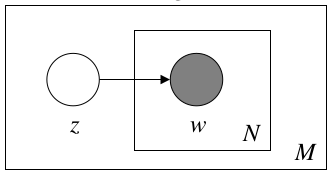
\includegraphics[scale=0.5]{chap2-img/graphicalmodel}
	\caption{نمومه‌ای از یک مدل گرافی \cite{blei2003latent}}
	\label{chap2-fig4}
\end{figure}

برای مثال در شکل
\ref{chap2-fig4}
که یک مدل گرافی ساده را نشان می‌‌دهد، مستطیل بیرونی
$M$
بار و مستطیل درونی به ازای هر بار تکرار مستطیل بیرونی
$N$
بار تکرار می‌‌شود. همچنین این مدل از دو متغیر تصادفی تشکیل شده که بین آن‌ها یک وابستگی شرطی نیز وجود دارد و یکی‌ از آن‌ها یک متغیر پنهان
($z$)
و دیگری یک متغیر قابل‌مشاهده
($w$)
می‌ باشد.
\section{مدل مخلوط}
در علم آمار یک مدل مخلوط\LTRfootnote{Mixture Model}
یک مدل احتمالاتی است که از آن برای نشان دادن وجود چند زیر جامعه\LTRfootnote{Subpopulation}
در یک جامعه‌ی بزرگتر بدون نیاز به داده‌ی قابل مشاهده برای شناسایی‌ و تشخیص آن زیر جامعه‌ها استفاده می‌‌‌شود. به بیان رسمی‌، یک مدل مخلوط متناظر با یک توزیع مخلوط\LTRfootnote{Mixture Distribution}
 است که توزیع‌های احتمالاتی مشاهده شده در یک جامعه‌ی کلی‌ یا جمعیت بزرگتر را نشان می‌‌دهد.
	
\section{تابع لجستیک}
تابع لجستیک\LTRfootnote{Logistic Function}
 یک منحنی متداول از خانواده‌ی منحنی‌های سیگمویدی\LTRfootnote{Sigmoid Curves}
  است. رابطه‌ی:
\begin{align}
	f(x) = \frac{L}{1+e^{-k(x-x_0)}}
	\label{eq1}
\end{align}
نشان دهنده یک تابع لجستیک است که در آن
$x_0$
نقطه میانی منحنی سیگمویدی روی محور
x
ها،
$L$
مقدار بیشینه منحنی در مثبت بی‌ نهایت و
$k$
برابر با شیب منحنی است.


 در شکل
\ref{fig3}
برای مقادیر x در بازه‌ی اعداد حقیقی‌ از منفی‌ بی‌ نهایت تا مثبت بی‌ نهایت نمودار این منحنی نشان داده شده است. تابع لجستیک در ادامه برای معرفی تابع
softmax
مورد استفاده قرار می‌‌گیرد.
\begin{figure}[!h]
	\centering
	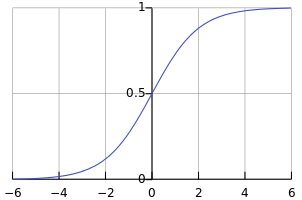
\includegraphics[scale=0.5]{chap2-img/logistic_function}
	\caption{تابع لجستیک در بازه‌ی اعداد حقیقی‌ از منفی‌ بی‌ نهیات تا مثبت بی‌ نهیات }
	\label{fig3}
\end{figure}

\section{تابع Softmax}
\label{chap2sec9}
در ریاضیات تابع
Softmax
که به آن تابع توانی‌ نرمال‌شده\LTRfootnote{Normalized Exponential Function}
 نیز می‌‌گویند، یک تابع لجستیک تعمیم یافته است که از آن برای نرم کردن یک بردار
K
بعدی مانند
\textbf{z}
متشکل از اعداد حقیقی‌ دلخواه به یک بردار
K
بعدی مانند
$\sigma(\textbf{z})$ 
تشکیل شده از اعداد حقیقی‌ بین بازه‌ی
$(0,1)$
به گونه‌ای که مجموع آنها برابر با ۱ باشد استفاده می‌‌کنند. رابطه‌ی
\begin{align}
	\sigma(\textbf{z}) = \frac{e^{z_i}}{\sum_{k=1}^{K}e^{z_k}} \quad\quad for\quad i = 1, ..., K
	\label{eq2}
\end{align}
معادله‌ی تابع
Softmax
را نشان می‌‌دهد. با توجه به خاصیت ذکر شده برای بردار حاصل از تابع
Softmax
در تئوری احتمال از این خروجی برای تعریف یک توزیع احتمالی که دارای
K
خروجی ممکن است استفاده می‌کنند. در بخش‌های بعدی از این تابع برای تعریف توزیع‌های احتمالی‌ برای موضوعات مختلف استفاده می‌‌کنیم.


\section{تابع گاما}
\label{chap2sec8}
تابع گاما\LTRfootnote{Gamma Function}
 که آن را با
$\Gamma$
نشان می‌‌دهند از تابع فاکتوریل مشتق شده است و برای یک عدد صحیح مثبت مقدار آن از رابطه‌ی
\begin{align}
	\centering
	\label{eq13}
	\Gamma(n) = (n-1)!
\end{align}
بدست می‌‌آید. تابع گاما در واقع برای تمام اعداد نامنفی حتی اعدد مختلظ نیز تعریف می‌‌شود. برای یک عدد مختلط با بخش حقیقی مثبت مقدار این تابع از رابطه‌ی
\begin{align}
	\centering
	\label{eq14}
	\Gamma(z) = \int_{0}^{\infty} x^{z-1}e^{-x}dx
\end{align}
بدست می‌‌آید.

\section{زنجیره‌ی مارکوف مونت کارلو}
\label{chap2sec6}
روش زنجیره‌ مارکوف مونت کارلو\LTRfootnote{Markov Chain Mont Carlo}
 که به اختصار آن را
MCMC
می‌ گویند، در کلاس روش‌های تولید نمونه از یک توزیع احتمالاتی قرار دارد. به زبان خیلی‌ ساده
MCMC
با ساختن یک زنجیر مارکوف برگشت‌پذیر\LTRfootnote{Reversible}
که در حالت تعادل توزیعی مشابه توزیع مورد نظر ما را دارد، از توزیع احتمالاتی نمونه تولید می‌‌کند. به بیان دیگر حالت زنجیر مارکوف، بعد از طی‌ کردن چند مرحله به عنوان یک نمونه از توزیع احتمالاتی مورد نظر در نظر گرفته می‌شود. کیفیت نمونه‌‌ی تولید شده توسط روش
MCMC
با تعداد مراحلی که زنجیر مارکوف اجرا می‌‌گردد رابطه‌ی مستقیم دارد و هرچه تعداد این مراحل بیشتر باشد نمونه‌ی بهتری بدست خواهد داد.

\section{الگوریتم یادگیری واگرایی مقابله}
\label{chap2sec7}
الگوریتم یادگیری واگرایی مقابله\LTRfootnote{Contrastive Divergence}
 اولین بار در سال ۲۰۰۲ توسط آقای هینتون
\cite{hinton2002training}
به عنوان یک الگوریتم یادگیری تقریبی بیشینه‌سازی مورد انتظار\LTRfootnote{Maximum Likelihood Approximation}
پیشنهاد گردید که در اینجا آن را به طور کامل توضیح می‌‌دهیم، و در ادامه خواهیم دید که پایه و اساس روش‌های یادگیری مدل‌های پیشین و پیشنهادی در این پایان‌‌نامه بر اساس همین الگوریتم هستند.

\subsection{الگوریتم واگرایی مقابله چیست و چرا به آن احتیاج داریم}
\label{chap2sec7sub1}

فرض کنید که قصد مدل‌سازی احتمال یک نقطه داده\LTRfootnote{Data Point}
 مانند
$x$
را با استفاده از یک تابع به شکل
$f(x;\theta)$
که در آن
$\theta$
یک بردار از پارامتر‌های مدل است را داریم. می‌‌دانیم که احتمال
$x$
که آن را به صورت
$p(x;\theta)$
نمایش می‌‌دهیم به ازای مجموع تمام حالت‌های
$x$
باید برابر با ۱ شود. بنابراین داریم:
\begin{align}
\centering
p(x;\theta) = \dfrac{1}{Z(\theta)}f(x;\theta)
\label{eg3}
\end{align}

که در آن
$Z(\theta)$
تابع قسمت‌بندی\LTRfootnote{Partition Function}
 است و به فرم
\begin{align}
\centering
Z(\theta) = \int f(x;\theta)dx
\label{eg4}
\end{align}
تعریف می‌شود. تابع قسمت‌بندی برای ما تضمین می‌‌کند که مقدار بدست آمده برای عبارت سمت چپ رابطه‌ی
\ref{eg3}
یک مقدار صحیح احتمالی‌ (بین ۰ و ۱) است
\cite{woodfordnotes}.

مجموعه پارامتر‌های مدل را که در اینجا با
$\theta$
نشان می‌‌دهیم، را با بیشینه کردن احتمال یک مجموعه‌‌ی آموزش\LTRfootnote{Training Set}
 از داده‌ها که آن را به صورت
$\textbf{X} = x_{1,...,K}$
تعریف می‌‌کنیم، یاد می‌‌گیریم. که در این حالت احتمال مجموعه آموزش از رابطه‌ی
\begin{align}
	\centering
	p(\textbf{X};\theta) = \prod_{k=1}^{K} \frac{1}{Z(\theta)} f(x_k;\theta)
	\label{eq5}
\end{align}
بدست می‌‌آید. یا با کمینه کردن مقدار منفی لگاریتم
$p(\textbf{X};\theta)$
که آن را با
$E(\textbf{X};\theta)$
نشان داده و انرژی مربوط به مدل تعریف می‌کنیم و از رابطه‌ی 
\begin{align}
	\centering
	E(\textbf{X};\theta) = \log Z(\theta) - \dfrac{1}{K} \sum_{i=1}^{K} \log f(x_i;\theta)
	\label{eq6}
\end{align}
محاسبه می‌شود، اقدام به یاد گیری پارامتر‌های مدل می‌‌کنیم.


در ادامه بر اساس نحوه‌ی تعریف تابع مدل احتمال، سه‌ حالت مختلف را بررسی‌ می‌‌کنیم و شرح می‌‌دهیم که الگوریتم یادگیری مقابله چیست، چرا و در چه حالتی به آن نیاز داریم.

اول حالتی را در نظر بگیرید که در آن تابع مدل احتمال\LTRfootnote{Probability Model Function}
 که آن را با
$p(x;\theta)$
نشان دادیم، تابع چگالی احتمال یک توزیع نرمال\LTRfootnote{Normal Distribution}
 به شکل
$N(x;\mu,\sigma)$
باشد. در این صورت مجموعه پارامتر‌های ما
$\theta = \{\mu,\sigma\}$
خواهد بود. بدیهی‌ است که انتگرال این تابع چگالی احتمال برابر با ۱ است. در نتیجه
$\log Z(\theta)=0$
می‌ شود. همچنین مشتق رابطه‌ی
\ref{eq6}
نسبت به
$\mu$
نشان می‌‌دهد که مقدار بهینه برای این متغیر
برابر با میانگین داده‌های آموزش است. همچنین مشتق رابطه‌ی
\ref{eq6}
این بار نسبت به
$\sigma$
نشان می‌‌دهد که مقدار بهینه برای این متغیر برابر با ریشه‌ی دوم واریانس داده‌های آموزش است.

در بعضی‌ مواقع مانند آنچه که در اینجا ذکر کردیم، روشی‌ وجود دارد که به صورت دقیق توانایی کمینه کردن تابع انرژی را دارد. برای درک بهتر، اگر تابع انرژی را در فضای پارامتر‌های مساله به صورت یک زمین مواج\LTRfootnote{Undulating Field}
در نظر بگیرید که هدف ما پیدا کردن پایین‌ترین نقطه در آن است، در این  صورت حالتی که در اینجا ذکر شد برابر است با زمانی‌ که در این زمین مواج همه چیز واضح و هوا آفتابی است و ما پایین‌ترین نقطه را مشاهده می‌‌کنیم و مستقیماً به سمت آن قدم می‌‌زنیم
\cite{woodfordnotes}.

برای حالت بعدی زمانی‌ را تصور کنید که در آن تابع مدل احتمال، برابر با مجموع
N
توزیع نرمال به شکل
\begin{align}
	\centering
	f(x;\theta)=\sum_{i=1}^N N(x;\mu_i,\sigma_i)
	\label{eg7}
\end{align}
باشد.
در این حالت مجموعه پارامترهای مدل به شکل
$\theta = \{\mu_{1,...,N},\sigma_{1,...,N} \}$ 
خواهد بود. این حالت مشابه زمانی‌ است که ما یک مدل مخلوط یا مجموعه‌ای از خبره‌ها 
\LTRfootnote{Mixture of Expert}
داشته باشیم که در آن وزن تمام افراد خبره برابر است. با توجه به این‌که انتگرال توزیع نرمال برابر با ۱ است، از رابطه
\ref{eg4}
داریم
$\log Z(\theta) = \log N$.
 در این حالت مشتق گرفتن از رابطه
\ref{eq6}
نسبت به هر یک از پارامتر‌های مدل، مدل جدیدی که وابسته به دیگر پارامتر‌های مدل است را تولید می‌‌کند. بنابراین مقدار بهینه برای پارامتر‌های مدل را به صورت مستقیم نمی‌‌توانیم محاسبه کنیم. راه جایگزین در این حالت استفاده از معادلات مشتقات جزئی‌ \LTRfootnote{Partial Differential}
و روش نزول گرادیانی\LTRfootnote{Gradient Descent}
 با جستجوی خطی‌\LTRfootnote{Line Search}
  است، که با استفاده از آن‌ها می‌‌توانیم نقطه کمینه محلی برای انرژی در فضای پارامتر‌های مدل را پیدا کنیم.

اگر به مثال خود برای حالت قبل باز گردیم، شرایط بیان شده در اینجا، یعنی‌ استفاده از نزول گرادیانی به همراه جستجوی خطی‌ مشابه زمانی‌ است که ما در هنگام شب به همراه یک مشعل در آن زمین مواج حضور داشته باشیم. همچنین ما توانایی احساس شیب نقطه‌ای که در آن ایستاده‌ایم را خواهیم داشت، یا می‌‌توانیم شیب این نقطه را نسبت به تمام جهت‌های اطرافمان تا فاصله‌ی اندکی‌ با استفاده از نور مشعل تعیین کنیم. بنابراین با تاباندن نور مشعل به جهتی‌ که برای حرکت انتخاب کرده‌ایم می‌‌توانیم پایین‌ترین نقطه در آن جهت را مشاهده کنیم به آن‌جا رفته و سپس جهت جدیدی را برای حرکت انتخاب کنیم
 \cite{woodfordnotes}.

 
 
 برای حالت سوم که حالت پایانی نیز است فرض کنید که ما تابع مدل احتمال را به صورت ضرب
 $N$
 توزیع نرمال به شکل
 \begin{align}
 	\centering
 	f(x;\theta)=\prod_{i=1}^N N(x;\mu_i,\sigma_i)
 	\label{eq8}
 \end{align}
 در نظر می‌‌گیریم.
این شرایط هم ارز با یک مدل ضرب خبره‌ها است. در این حالت تابع قسمت‌بندی دیگر مقدار ثابتی نخواهد داشت و بسته به مقادیر پارامتر‌های توزیع‌های نرمال مقدار آن متفاوت خواهد بود. برای مثال زمانی‌ که مدل فقط شامل دو توزیع نرمال است و برای هر دوی آن‌ها
 $\sigma = 1$
 را در نظر بگیرید. اگر
 $\mu_1 = -\infty$
 و
 $\mu_2 = \infty$
 آنگاه
 $Z(\theta) = 0$
 می‌ شود. در حالی‌ که اگر
 $\mu_1 = \mu_2 = 0$
 آنگاه
 $Z(\theta) = \frac{1}{2}\sqrt{\pi}$
 می‌شود. بنابراین بسته به مقادیری که برای پارامتر‌های مدل انتخاب می‌‌شوند مقدار
 $Z(\theta)$
 متغیر خواهد بود.
 
 اگرچه در این حالت محاسبه‌‌ی دقیق تابع قسمت‌بندی امکان پذیر است، اما شرایطی را در نظر بگیرید که در آن تابع مدل احتمال به گونه‌ای باشد که محاسبه‌ی‌ انتگرال در رابطه
\ref{eg4}
 از نظر جبری غیرعملی\LTRfootnote{Intractable}
 ‌ باشد. در این حالت برای ارزیابی رابطه
\ref{eq6}
 ما نیاز خواهیم داشت از انتگرال‌گیری عددی\LTRfootnote{Numerical Integration}
 استفاده کنیم. همچنین باید از مشتقات متناهی برای محاسبه گرادیان در یک نقطه‌ی داده شده در فضای پارامتر‌های مساله و همچنین روش‌های نزول گرادیانی برای پیدا کردن کمینه محلی استفاده کنیم. برای فضاهای داده‌ای و پارامتری با ابعاد بالا زمان این انتگرال‌گیری فلج کننده\LTRfootnote{Crippling}
 خواهد بود. شرایط بیان شده تا اینجا منجر به وضعیتی می‌‌گردد که در آن ما تلاش می‌‌کنیم یک تابع انرژی را کمینه کنیم در حالی‌ که توانایی ارزیابی کردن آن را نداریم.
 
 اینجا زمانی‌ است که الگوریتم واگرایی مقابله به ما کمک می‌‌کند. اگر چه که ما نمی‌‌توانیم خود تابع انرژی را ارزیابی کنیم اما الگوریتم
 CD
 برای ما راهی‌ را مهیا می‌‌کند که می‌توانیم به کمک آن گرادیان تابع انرژی را تخمین بزنیم. اگر به مثال خود برای حالت‌های قبل بازگردیم، در شرایط بیان شده برای حالت نهایی ما خودمان را در همان زمین مواج بدون هیچ‌گونه امکانات و توانایی خاصی خواهیم یافت (ما نمی‌‌توانیم انرژی را محاسبه کنیم)، در نتیجه ما امکان تشخیص ارتفاع و شیب در هیچ یک از نقطه‌های اطرافمان را نسبت به نقطه‌ای که در آن ایستاده‌ام را نداریم. الگوریتم
 CD
 در این حالت به ما یک حس تعادل می‌‌دهد و به ما این اجازه را می‌‌دهد که شیب نقطه‌ای از زمین که در زیر پایمان قرار دارد را تشخیص دهیم. حال با برداشتن قدم‌های بسیار کوچک در جهتی‌ که بیشترین کاهش شیب را داریم ما توانایی پیدا کردن راه خودمان به سمت کمینه‌ی محلی را خواهیم داشت
 \cite{woodfordnotes}.
 
\subsection{الگوریتم واگرایی مقابله چگونه کار می‌کند}
همان طور که در بخش
\ref{chap2sec7sub1}
توضیح داده شد، الگوریتم
CD
با توجه مجموعه پارامترهای مدل و داده‌های آموزش، گرادیان تابع انرژی را برای ما تخمین می‌‌زند.  در رابطه‌ی
\begin{align}
	\centering
	\label{eq9}
	\dfrac{\partial E(\textbf{X};\theta)}{\partial \theta} &= \dfrac{\log Z(\theta)}{\partial \theta} - \dfrac{1}{K}\sum_{i=1}^K\dfrac{\partial \log f(x_i;\theta)}{\partial \theta}\\\nonumber
	&= \dfrac{\log Z(\theta)}{\partial \theta} - \left\langle \dfrac{\partial \log f(x_i;\theta)}{\partial \theta}\right\rangle_\textbf{X}
\end{align}
 با استفاده از مشتقات جزئی فرمول محاسبه‌ی گرادیان را از را رابطه
\ref{eq6}
 بدست می‌‌آوریم. در رابطه‌ی
\ref{eq9}
 نماد
$\langle \star \rangle_\textbf{X}$
 نشان دهنده مقدار مورد انتظار برای
$\star$
 با توجه به توزیع داده‌ی
\textbf{X}
 می‌ باشد.

اولین ترم در سمت راست رابطه‌‌ی
\ref{eq9}
از تابع قسمت‌بندی مشتق می‌گردد و همانطور که در رابطه‌ی
\ref{eg4}
مشاهده می‌‌گردد شامل یک انتگرال‌گیری بر روی
$x$
است. با جایگذاری این رابطه به رابطه‌ی
\begin{align}
	\centering
	\label{eq10}
	\dfrac{\partial\log Z(\theta)}{\partial \theta} &= \dfrac{1}{Z(\theta)}\dfrac{\partial Z(\theta)}{\partial(\theta)}\\ \nonumber
	&=\dfrac{1}{Z(\theta)}\dfrac{\partial}{\partial(\theta)}\int f(x;\theta)dx\\ \nonumber
	&=\dfrac{1}{Z(\theta)}\int \dfrac{\partial f(x;\theta)}{\partial(\theta)}dx\\	\nonumber
	&=\dfrac{1}{Z(\theta)}\int f(x;\theta) \dfrac{\partial \log f(x;\theta)}{\partial(\theta)}dx\\ \nonumber
	&= \int p(x;\theta) \dfrac{\partial \log f(x;\theta)}{\partial(\theta)}dx\\ \nonumber
	&= \left\langle \dfrac{\partial \log f(x;\theta)}{\partial(\theta)}\right\rangle_{p(x;\theta)}
\end{align}
می‌رسیم. همان‌طور که در بخش
\ref{chap2sec7sub1}
بحث کردیم محاسبه‌ی این انتگرال در حالت کلی‌ از نظر جبری غیر عملی‌ است. اما در رابطه‌ی
\ref{eq10}
روشن است که می‌‌توانیم با نمونه گرفتن از توزیع
$p(x;\theta)$
این انتگرال را به صورت عددی تقریب بزنیم.
از آن‌جا که ما مقدار دقیق تابع قسمت‌بندی را نمی‌‌دانیم لذا نمی‌‌توانیم به صورت مستقیم از
$p(x;\theta)$
نمونه تولید کنیم. اما با استفاده از تعداد زیادی چرخه نمونه‌برداری
MCMC
که در بخش
\ref{chap2sec6}
معرفی‌ شد می‌توانیم توزیع داده‌های آموزش  را به توزیع پیشنهاد شده برای داده‌ها تبدیل کنیم. این تبدیل از آنجایی امکان پذیر است که تنها شامل محاسبه‌ی نسبت دو توزیع احتمالی‌ به صورت
$\frac{p(x';\theta)}{p(x;\theta)}$
است و تابع قسمت‌بندی از معادله حذف می‌‌گردد. در اینجا
$\textbf{X}^n$
نشان دهنده‌ی داده‌های آموزش است که با
$n$ 
چرخه‌ی نمونه‌برداری
MCMC
تبدیل یافته‌اند، با توجه به این می‌‌توانیم تعریف کنیم‌:
$\textbf{X}^0 = \textbf{X}$.
با جایگذاری این روابط در رابطه‌ی
\ref{eq9}
به رابطه‌ی
\begin{align}
	\centering
	\label{eq11}
	\dfrac{\partial E(\textbf{X};\theta)}{\partial \theta} = \left\langle \dfrac{\partial \log f(x; \theta)}{\partial \theta} \right\rangle_{\textbf{X}^{\infty}} - \left\langle \dfrac{\partial \log f(x;\theta)}{\partial \theta}\right\rangle_{\textbf{X}^0}
\end{align}
می‌ رسیم.

تعداد زیاد چرخه‌‌ی نمونه‌برداری
MCMC
برای محاسبه‌ی یک گرادیان صحیح تنها مانع محاسباتی باقی‌ مانده است که باید بر آن غلبه کنیم. هینتون بیان کرد که تنها تعداد کمی چرخه‌ی نمونه‌برداری
MCMC
برای محاسبه‌ی یک گرادیان تقریبی نیاز خواهد بود، و بعد از تعداد کمی‌ تکرار توزیع داده‌های آموزش به سمت توزیع پیشنهاد شده شروع به حرکت می‌‌کند و جهتی‌ را که در آن داد‌ه‌ها بهتر مدل می‌شوند را نشان می‌‌دهد
\cite{hinton2002training}\cite{carreira2005contrastive}.
پیاده‌سازی‌های عملی‌ نشان داد که تنها یک چرخه‌ی نمونه‌برداری
MCMC
برای همگرایی الگوریتم به مقدار بیشینه مورد انتظار کفایت می‌‌کند
\cite{carreira2005contrastive}.
در نتیجه به منظور کمینه کردن تابع انرژی رابطه‌ی به روز‌رسانی کردن مجموعه پارامتر‌های ما به شکل رابطه‌ی
\begin{align}
	\centering
	\label{eq12}
	\theta_{t+1} = \theta_t + \eta \left(  \left\langle \dfrac{\partial \log f(x; \theta)}{\partial \theta} \right\rangle_{\textbf{X}^0} - \left\langle \dfrac{\partial \log f(x;\theta)}{\partial \theta}\right\rangle_{\textbf{X}^1}  \right) 
\end{align}
می‌گردد که در آن
$\eta$
ضریب یادگیری است و باید بر اساس زمان همگرایی و ثبات یادگیری الگوریتم به صورت تجربی‌ مشخص گردد.

\section{کیسه‌ی کلمات}
\label{chap2sec10}
مفهوم کیسه‌ی کلمات\LTRfootnote{Bag of Words}
 بیشتر در مباحث مربوط به پردازش زبان طبیعی و بازیابی اطلاعات
مورد استفاده قرار می‌‌گیرد و از آن به عنوان راهی‌ برای نمایش داده استفاده می‌‌کنند. در این روش هر جمله و یا هر سند به صورت کیسه‌ای از کلماتش که در واقع برداری از اعدد صحیح هستند نشان داده می‌‌شود. در این بردار ترتیب کلمات و اصول و قواعد گرامری رعایت نمی‌‌شود و تنها شامل تعداد تکرار کلمات متمایز و مختلف در جمله یا سند  متناظرش است. تعداد تکرار هر کلمه در روش کیسه کلمات به عنوان یک ویژگی‌ برای هر سند یا جمله در نظر گرفته می‌‌شود.

برای مثال دو متن زیر که به ترتیب دارای دو و یک جمله می‌باشند را در نظر بگیرید:


\begin{latin}
\begin{enumerate}
	\item John likes to watch movies. Mary likes movies too.
	\item John also likes to watch football games.
\end{enumerate}
\end{latin}
\vspace{-0.4cm}

برای نشان دادن این دو سند با استفاده از روش کیسه‌ی‌ کلمات اینگونه عمل می‌‌کنیم:
\vspace{-0.4cm}
\begin{enumerate}
	
	\item  شروع به پیمایش متن‌ها کرده و تمام کلمات متمایز را مشخص می‌کنیم.
	\vspace{0.1cm}
	\begin{latin}
		"John", "likes", "to", "watch", "movies", "also", "football", "games", "Mary", "too"
	\end{latin}
	\vspace{-0.4cm}
	
	\item کلمات متمایز را شماره‌گذاری می‌‌کنیم. در واقع یک لغت‌نامه تشکیل می‌‌دهیم که در آن هر عدد متناسب با یک لغت متمایز است.
	\vspace{0.1cm}
	\begin{latin}
		John=1, likes=2, to=3, watch=4, movies=5, also=6, football=7, games=8, Mary=9, too=10
	\end{latin}
	\vspace{-0.4cm}
	
	\item تمام اسناد را با برداری به طول ثابت نشان می‌‌دهیم. اندازه‌ی  این بردار برابر با بزرگترین اندیس کلمات در لغت‌نامه‌ی ساخته شده در مرحله‌ی قبل است ، و هر درایه‌ی آن متناظر با لغتی با همان اندیس در لغات‌نامه‌ی ساخته شده است.
	
	\item برای هر سند بردار متناظر با آن را تشکیل می‌‌دهیم و تعداد تکرار کلمات مختلف لغت‌نامه را در بردار نشان می‌‌دهیم.
	\vspace{0.1cm}
	\begin{latin}
		\begin{enumerate}
			\item $\{1, 2, 1, 1, 2, 0, 0, 0, 1, 1\}$
			\item $\{1, 1, 1, 1, 0, 1, 1, 1, 0, 0\}$
		\end{enumerate}
	\end{latin}
	\vspace{-0.4cm}
		
\end{enumerate}

\section{موضوع}
در حوزه‌ی پردازش زبان طبیعی یک موضوع به مجموعه یا خوشه‌ای\LTRfootnote{Cluster}
از کلمات متمایز گفت می‌‌شود که از نظر معنایی به یکدیگر نزدیک هستند و در یک دسته قرار می‌‌گیرند. برای مثال در شکل
\ref{chap2-tb1}
چهار خوشه از کلمات را مشاهده می‌‌کنید که از نظر معنایی به هم نزدیک هستند و می‌‌توانیم به ترتیب موضوع‌های الکترونیکی، فضایی، ورزشی و مذهبی را به آن‌ها اختصاص دهیم.
\begin{table}[!h]
	\centering
	\begin{latin}
	\begin{tabular}{|c|c|c|c|}
		\hline
		card 	 & shuttle 		& team 	   & christianity\\
		driver 	 & orbit 		& games    & god\\
		drivers  & lunar 		& seasons  & pgp\\ 
		bus		 & spacecraft 	& baseball & jesus\\ 
		video	 & nasa  		& players  & bible\\ 
		vga		 & space 		& game     & faith\\ 
		monitor  & launch 		& hockey   & muslim\\ 
		ibm   	 & saturn  		& play 	   & christ\\ 
		cards	 & billion		& teams    & atheist\\
		ram    	 & satellite	& sale     & christians\\
		\hline
	\end{tabular}
	\end{latin}
	\caption{نمونه‌ی چهار موضوع مختلف}
	\label{chap2-tb1}
\end{table}

\section{مدل‌ موضوعی}
\label{chap2sec12}
مدل‌های موضوعی یک کلاس جدید از روش‌های آنالیز متن\LTRfootnote{Text Analysis}
هستند که به تازگی به صورت گسترده مورد توجه پایان‌‌نامهگران حوزه‌های مختلف مانند پردازش زبان طبیعی، علوم اجتماعی، اقتصاد و  غیره قرار گرفته‌اند 
\cite{mohr2013introduction}\cite{blei2012probabilistic}.
  در مباحث مربوط به یادگیری ماشین و پردازش زبان طبیعی یک مدل موضوعی یک دسته از مدل‌های آماری است که برای کشف و نمایش یک چکیده\LTRfootnote{Abstract}
  از موضوع‌هایی که در یک مجموعه از اسناد\LTRfootnote{Corpus}
   وجود دارد به کار می‌رود 
\cite{zheng2014topic}\cite{blei2003modeling}.
   مهمترین ویژگی این مدل‌ها که باعث تمایز آن‌ها از دیگر مدل‌ها می‌‌گردد، روند کاملا اتوماتیک و خودکار آن‌ها برای تبدیل محتوای یک مجموعه سند متنی که این مجمومه سند می‌‌تواند بسیار بزرگ باشد به دسته‌هایی با معنا و مفهوم که "موضوع‌ها" نامیده می‌‌شوند، است
\cite{mohr2013introduction}.

الگوریتم‌ها و روش‌های موجود در این حوزه این روند را با کمترین دخالت انسانی‌ و به صورت کاملا خودکار انجام می‌‌دهند و همین امر موجب می‌‌گردد که به صورت قابل ملاحظه‌ای به روش‌های پیشین موجود در این زمینه ترجیح داده شوند. چرا که بیشتر روش‌های موجود در این زمینه نیاز به دخالت و نظارت یک عامل انسانی‌ در تمام مراحل اجرا را دارند. در مدل‌های موضوعی هیچ دانش اولیه‌ای در رابطه با نوع دسته‌ها یا موضوع‌های موجود در مجموعه سند داده نمی‌‌شود و تنها تعداد موضوع‌های مورد نظر به مدل داده می‌‌شود و پس از اتمام روند مدل‌سازی این موضوع‌ها به صورت توزیع‌های احتمالاتی بر روی کلمات متمایز موجود در مجموعه سند مشخص می‌‌شوند
\cite{mohr2013introduction}.

اما بحث مدل‌های موضوعی تنها به داده‌های متنی خلاصه نمی‌شود، به طور مثال در مباحث مربوط به پردازش تصویر\LTRfootnote{Image Processing}
و استخراج ویژگی\LTRfootnote{Feature Extraction}
از تصویر و یا ارایه‌ی تصویر به صورت فشرده می‌‌توان در ابتدا با استفاده از الگوریتم‌ها و روش‌های موجود در زمینه‌ی پردازش تصویر به تبدیل هر تصویر به یک سند متنی پرداخت و سپس با اجرای مدل‌های موضوعی بر روی سند متنی بدست آمده نتیجه‌ی مورد نیاز را به خوبی‌  بدست آورد
\cite{mohr2013introduction}.

اینکه این مدل‌ها به چه صورت عمل می‌‌کنند و بر چه اساسی‌ موضوع‌های موجود در یک مجموع سند را برای ما مدل می‌‌کنند یا به صورت کلی‌ در پاسخ به این سوال که تئوری و ایده‌ی اصلی‌ برای این مدل‌ها کدام است را می‌‌توان در یک پاسخ ساده خلاصه کرد. تمام این مدل‌ها بر اساس این فرضیه ساخته می‌‌شوند که معانی و مفاهیم با یکدیگر مرتبط هستند. به بیان دیگر به طور مثال در صحبت‌های روزمره مفاهیم و کلماتی که به صورت ذاتی در مورد یک موضوع خاص هستند یک مجموعه یا خوشه از کلمات به خصوصی را شامل  می‌شوند. بنابراین یک موضوع خاص می‌‌تواند به صورت مجموعه‌ای از کلماتی‌ در نظر گرفته شود که از نظر معنایی به هم نزدیک هستند و تمایل دارند که در یک مکالمه یا یک نوشتار زمانی‌ که در مورد آن موضوع خاص بحث می‌‌شود در کنار هم تکرار شوند و رخ دهند. توجه به این نکته ضروری است که از آنجا که مدل‌های موضوعی با کیسه‌ی کلمات کار می‌‌کنند در نتیجه تکرار و رخداد کلمات در کنار یکدیگر را به عنوان ویژگی‌ مورد توجه قرار می‌‌دهند و از پیچیدگی‌های دیگر زبانی ماند قواعد گرامری، دستوری، نحوی و غیره صرف نظر می‌‌کنند. اگرچه در تعدادی از مدل‌های موجود در این زمینه به این پیچیدگی‌های زبانی نیز اندکی توجه گردیده است اما در بیشتر این مدل‌ها از این پیچیدگی‌‌ها صرف نظر می‌‌شود. در نتیجه هدف نهایی از مدل‌سازی موضوعی آنالیز خوشه‌های مختلف کلمات و تشخیص کلماتی‌ است که از نظر معنایی به هم نزدیک هستند و تمایل دارند در کنار یکدیگر تکرار شوند و یک موضوع خاص را شکل دهند
\cite{mohr2013introduction}.
در مدل‌سازی موضوعی فرض بر این است که هر سند شامل چند موضوع مختلف است که هرکدام از این موضوع‌ها به صورت یک توزیع احتمالاتی بر روی کلمات بخصوصی هستند
\cite{steyvers2007probabilistic}.

برای مثال در شکل
\ref{fig2}
نمونه‌ای از یک مدل‌سازی موضوعی را مشاهده می‌‌کنید. در این شکل چهار موضوع با رنگ‌های مختلف به همراه احتمال رخ داد کلمات مرتبط با آن نشان داده شده اند. همچنین می‌‌توان نحوه‌ی تکرار این کلمات در متن اصلی‌ را مشاهده کرد که هر کلمه با رنگ مرتبط با یک موضوع مشخص شده است.
\begin{figure}[!t]
	\centering
	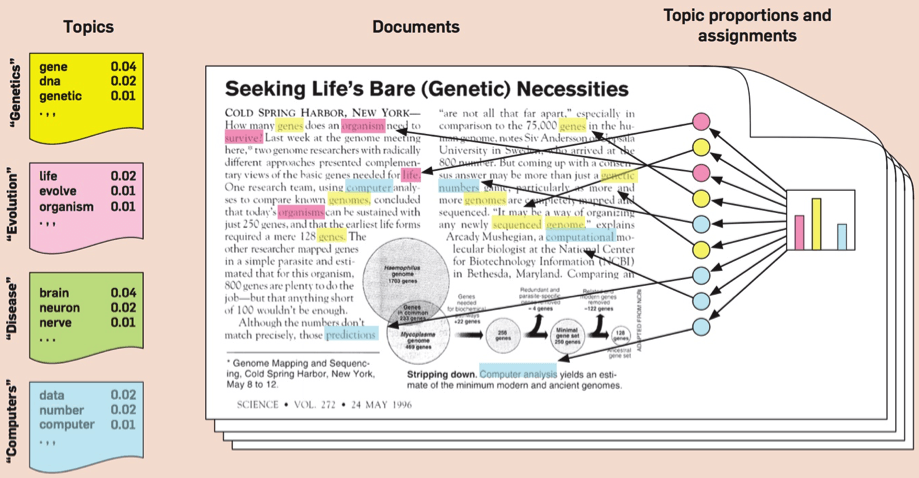
\includegraphics[scale=0.5]{chap2-img/topic_model_example2}
	\caption{نمونه‌ای از یک مدل‌سازی موضوعی}
	\label{fig2}
\end{figure}


\section{آنالیز احساس}
منظور از آنالیز احساس یا کاوش عقاید مشخص کردن اطلاعات مفهومی‌\LTRfootnote{Subjective Information}
مانند نظرات، نگرش‌ها و احساس موجود در متن نوشته شده است. در آنالیز احساس در حوزه‌ی ‌‌پردازش زبان طبیعی و پردازش متن ما به دنبال ابزار هایی هستیم که این اطلاعات مفهومی‌ را به صورت خود کار از متن یا مجموعه اسناد استخراج کند و احساس موجود در متن را برای ما مشخص کند
\cite{lin2012weakly}\cite{pang2008opinion}.
 می‌توان احساس موجود در یک متن را در سه‌ دسته قرار داد: مثبت، منفی‌ و بی‌طرف.

هدف نهایی در آنالیز احساس مشخص کردن همین امر است  که یک متن از نظر احساسی‌ مثبت، منفی‌ و یا بی‌ طرف است. در بحث تشخیص همزمان موضوعی و احساس از یک متن فرض بر این است که در یک سند متنی در مورد چندین موضوع صحبت شده است و هرکدام از این موضوع‌ها می‌‌توانند احساس خاص مربوط به خود را داشته باشند. به طور مثال فرض کنید که شما یک محصول الکترونیکی جدید مانند لپ‌تاپ خریداری کرده‌اید. حال اگر شما یک بازبینی\LTRfootnote{Review}
برای این لپ‌تاپ بنویسید، این نوشته شامل موضوعات مختلفی‌ خواهد بود چرا که یک لپ‌تاپ شامل بخش‌های مختلفی‌ نظیر صفحه نمایش، باطری، حافظه و ... است و در بازبینی نوشته شده هر کدام از این‌ها به عنوان یک موضوع مجزا در نظر گرفته می‌‌شوند. حال هرکدام از این موضوع‌ها می‌‌توانند احساس خاص مربوط به خود را داشته باشند، به طور مثال شما از حافظه لپ‌تاپ راضی‌ هستید ولی‌ در مقابل صفحه نمایش آن انتظارات شما را برآورده نکرده است، در اینجا احساس شما به موضوع حافظه مثبت و به موضوع صفحه نمایش منفی‌ خواهد بود. هدف ما در تشخیص همزمان موضوع و احساس از داده‌های متنی نیز به همین شکل است که علاوه بر تشخیص موضوع‌های مورد بحث، احساس همراه با هرکدام را نیز تشخیص دهیم.



 	%chap 3
\chapter{بررسی پژوهش‌های پیشین}
\thispagestyle{empty}
\section{مقدمه}
در این فصل به مرور و بررسی روش‌ها و پژوهش‌های موجود پیشین در زمینه‌ی  تخمین توزیع\LTRfootnote{Distribution Estimation}، 
استخراج اطلاعات\LTRfootnote{Information Extraction}
از متن، بازیابی اطلاعات و مدل‌سازی  موضوع می‌پردازیم. در همین راستا  به بررسی‌ مهم‌ترین مدل‌ها و روش‌های موجود در زمینه‌ی مدل‌سازی موضوع، مدل‌سازی موضوع و احساس به صورت همزمان و همچنین دسته‌ی خاصی‌ از مدل‌های موضوعی که به آن‌ها چندحالته گفته می‌‌شود می‌‌پردازیم. هدف از معرفی‌ این روش‌ها آشنایی با کار‌های انجام شده در زمینه‌ی مربوطه تا به امروز و درک هرچه بهتر ایده و علت انجام این پژوهش است. در این فصل روش‌های موجود را از چندین زاویه مورد نقد و بررسی‌ قرار می‌‌دهیم و بسته به ساختار، نحوه‌ی عملکرد، نوع داده‌ی ورودی و سیر تکاملی، آن‌ها را در چندین کلاس طبقه‌بندی می‌‌کنیم.

در بررسی‌ روش‌ها و مدل‌های موجود از دید ساختاری، می‌‌توان آن‌ها را در دو دسته کلی‌ طبقه‌بندی کرد. یک مدل‌های بر پایه‌ی شبکه‌های عصبی و دو مدل‌های گرافی‌. در بحث مدل‌سازی موضوع، مدل‌های گرافی‌ نسبت به مدل‌های شبکه‌های عصبی از قدمت بیشتری برخوردار هستند. مهمترین مدلی‌ که در این دسته وجود دارد و در بخش 
\ref{chap3sec3}
آن را دقیق‌تر بررسی‌ می‌‌نماییم مدل معروف تخصیص دیریکله‌ی پنهان است
 (LDA)
  که در سال ۲۰۰۳ توسط
Blei
و همکاران 
\cite{blei2003latent}
ارائه گردید، و پس آن به عنوان پایه‌ی مدل‌سازی موضوعی در بخش مدل‌های گرافی قرار گرفت. دسته‌ی دیگر مدل‌های موضوعی موجود از نظر ساختار آن‌هایی هستند که بر پایه‌ی شبکه‌های عصبی مصنوعی هستند و اولین بار در سال ۲۰۰۹ توسط
Hinton
و
Salakhutdinov \cite{hinton2009replicated}
معرفی‌ شدند. در بخش‌ 
\ref{chap3sec3}
با هر کدام از این دو دسته بیشتر آشنا می‌‌شویم و روش‌های موجود در آن‌ها را معرفی می‌کنیم. جدول
\ref{tabel3-1}
ساختار تمام روش‌های معرفی‌ شده در این فصل که در ادامه به صورت مفصل به هر کدام می‌پردازیم را نشان می‌‌دهد.
\begin{table}[!t]
	\centering
	\begin{latin}
		\begin{tabular}{|c|c|c|}
			\hline
			                               & Graphical Model & Neural Network Model \\ \hline
			          Latent Semantic Indexing(LSI)            &     $\star$     &  \\ \hline
			   probabilistic Latent Semantic Indexing(pLSI)    &     $\star$     &  \\ \hline
			         Latent Dirichlet Allocation(LDA)          &     $\star$     &  \\ \hline
			    Joint Sentiment/Topic Model Detection(JST)     &     $\star$     &  \\ \hline
			   Aspect and Sentiment Unification Model(ASUM)    &     $\star$     &  \\ \hline
		 Supervised Joint Aspect and Sentiment Model(SJASM)    &     $\star$     &  \\ \hline
			Neural Autoregressive Distribution Estimator(NADE) &                 &       $\star$        \\ \hline
			         Restricted Boltzman Machine(RBM)          &                 &       $\star$        \\ \hline
			              Replicated Softmax(RS)               &                 &       $\star$        \\ \hline
			              Document NADE(DocNADE)               &                 &       $\star$        \\ \hline
			          Supervised DocNADE(SupDocNADE)           &                 &       $\star$        \\ \hline
		\end{tabular}
	\end{latin}
	\caption{دسته‌بندی مدل‌های پیشین از نظر ساختار}
	\label{tabel3-1}
\end{table}


از نظر نحوه‌ی عملکرد مدل‌های پیشین را در سه‌  کلاس مختلف قرار می‌‌دهیم. دسته‌ي اول روش‌هایی که تنها به مدل‌سازی موضوع می‌‌پردازند و آن‌ها را به عنوان روش‌های مدل‌سازی موضوعی معرفی‌ می‌‌کنیم. دسته‌ی دوم روش‌هایی که تنها به تشخیص احساس و دانش مفهومی‌ از داده‌های ورودی می‌‌پردازند. اگرچه باید توجه داشت که مدل‌های موجود در زمینه تشخیص احساس در دسته‌ی مدل‌های موضوعی قرار نمی‌‌گیرند و بیشتر شامل مدل‌های یادگیری ماشین هستند که یک طبقه‌بندی\LTRfootnote{Classification}
 دو حالته (مثبت و منفی‌) یا سه‌ حالته (منفی‌، مثبت و بی‌ طرف) را انجام می‌‌دهند. 
و در دسته‌‌ي سوم که دسته‌ی آخر از نظر نحوه‌ی عملکرد است روش‌هایی را بررسی می‌کنیم که به صورت همزمان به مدل‌سازی موضوع و احساس بر روی داده‌ی ورودی می‌‌پردازند.  در جدول
\ref{tabel3-2}
نوع مدل‌های معرفی‌ شده در این فصل از نظر نحو‌ه‌ی عملکرد مشاهده می‌‌شود.
\begin{table}[!h]
	\centering
	\begin{latin}
		\begin{tabular}{|c|c|c|}
			\hline
			                         & Topic Model & Sentiment/Topic Model \\ \hline
			       Latent Semantic Indexing(LSI)         &   $\star$   &  \\ \hline
			probabilistic Latent Semantic Indexing(pLSI) &   $\star$   &  \\ \hline
			      Latent Dirichlet Allocation(LDA)       &   $\star$   &  \\ \hline
			 Joint Sentiment/Topic Model Detection(JST)  &             &        $\star$        \\ \hline
			Aspect and Sentiment Unification Model(ASUM) &             &        $\star$        \\ \hline
      Supervised Joint Aspect and Sentiment Model(SJASM) &             &        $\star$        \\ \hline
			           Replicated Softmax(RS)            &   $\star$   &  \\ \hline
			           Document NADE(DocNADE)            &   $\star$   &  \\ \hline
		\end{tabular}
	\end{latin}
	\caption{دسته‌بندی مدل‌های پیشین از نظر نحوه‌ی عملکرد}
	\label{tabel3-2}
\end{table}



روش‌های پیشین از نظر نوع داده‌ی ورودی در دو کلاس متفاوت قرار می‌‌گیرند. یک گروه روش‌هایی که تنها یک نوع داده را به عنوان ورودی قبول می‌‌کنند. منظور از یک مدل داده این است که روش‌های موجود توانایی عمل کردن به صورت همزمان بر روی چند مد مختلف از داده‌ها را ندارند، و داده‌های ورودی تنها باید یک حالت داشته باشند، مثلا تنها متن و یا تنها تصویر باشند و نمی‌‌توانند ترکیبی‌ از این‌ها باشند. دسته‌ی دوم که آن‌ها را مدل‌های چندحالته می‌‌شناسیم مدل‌هایی هستند که با داده‌های چندوجهی کار می‌‌کنند. منظور از داده‌های چندوجهی آن‌هایی هستند که شامل ترکیب چند حالت مختلف از داده هستند، برای مثال ترکیب متن و تصویر و یا ترکیب تصویر و صدا. در جدول
\ref{tabel3-3}
تفاوت بین روش‌های موجود از نظر نوع داد‌ه‌ی ورودی مشخص شده است.
\begin{table}[!b]
	\centering
	\begin{latin}
		\begin{tabular}{|c|c|c|}
			\hline
			                            & Unimodal & Multimodal \\ \hline
			          Latent Semantic Indexing(LSI)            & $\star$  &  \\ \hline
			   probabilistic Latent Semantic Indexing(pLSI)    & $\star$  &  \\ \hline
			         Latent Dirichlet Allocation(LDA)          & $\star$  &  \\ \hline
			    Joint Sentiment/Topic Model Detection(JST)     & $\star$  &  \\ \hline
			   Aspect and Sentiment Unification Model(ASUM)    & $\star$  &  \\ \hline
            Supervised Joint Aspect and Sentiment Model(SJASM) & $\star$  &  \\ \hline
			Neural Autoregressive Distribution Estimator(NADE) & $\star$  &  \\ \hline
			         Restricted Boltzman Machine(RBM)          & $\star$  &  \\ \hline
			              Replicated Softmax(RS)               & $\star$  &  \\ \hline
			              Document NADE(DocNADE)               & $\star$  &  \\ \hline
			          Supervised DocNADE(SupDocNADE)           &          &  $\star$   \\ \hline
		\end{tabular}
	\end{latin}
	\caption{دسته‌بندی مدل‌های پیشین از نظر داده‌ی ورودی}
	\label{tabel3-3}
\end{table}

از نقطه‌نظر سیر تکاملی می‌‌توان روش‌های موجود را در سه‌ سطح: یک مدل‌های تخمین زننده‌ی توزیع، دو روش‌های مدل‌سازی موضوع و سه مدل‌های تشخیص همزمان موضوع و احساس به صورت مشترک قرار داد. البته لازم به ذکر است که روش‌های تخمین توزیع که در اینجا مطرح می‌‌گردند و در بحث پردازش زبان طبیعی مورد استفاده قرار می‌‌گیرند به تنهایی در دسته‌ی مدل‌های موضوعی قرار نمی‌‌گیرند اما پایه و اساس بسیاری از مدل‌های موضوعی هستند و لذا در بخش
\ref{sec2}
آن‌ها را معرفی‌ کرده و به صورت مختصر توضیح می‌‌دهیم.



\section{مدل‌های تخمین توزیع احتمالی}
\label{sec2}
اولین گروه از مدل‌های پیشین که به بررسی‌ آن‌ها می‌‌پردازیم روش‌هایی هستند که به تخمین توزیع‌های احتمالی‌ موجود در داده‌های ورودی می‌‌پردازند. در بخش‌های
\ref{chap3sec2sub1}
و
\ref{chap3sec2sub2}
به ترتیب مدل‌های "ماشین بلتزمن محدود\LTRfootnote{Restricted Boltzman Machine}"
(RBM)
\cite{smolensky1986information}\cite{freund1994unsupervised}\cite{hinton2002training}
 و همچنین مدل "شبکه‌‌ی عصبی خود رگرسیو تخمین‌زننده‌ی توزیع\LTRfootnote{Neural Autoregressive Distribution Estimator}"
(NADE)
  که در سال
۲۰۱۱
توسظ 
Larochelle
و
Murray \cite{larochelle2011neural}
معرفی شد، را بررسی می‌کنیم . این دو مدل از مهمترین روش‌های موجود در زمینه تخمین توزیع در بحث پردازش زبان طبیعی هستند. دلیل اهمیت و معرفی‌ این روش‌ها این می‌‌‌باشد که مدل‌هایی که در بخش‌های بعدی معرفی‌ می‌‌شوند گسترش یافته‌ی این روش‌ها هستند و از تغییر در ساختار این مدل‌ها بدست می‌‌آیند.

	
	
	\subsection{مدل ماشین بلتزمن محدود}
	\label{chap3sec2sub1}
	مدل ماشین بلتزمن محدود که به اختصار آن را
	RBM
	می‌ نامیم یک مدل شبکه عصبی بدون‌نظارت برای تخمین توزیع داده‌های ورودی باینری است. 
	RBM
	در دسته مدل‌های احتمالاتی مولد
	 (بخش 
	 \ref{chap2sec3sub2})
	 قرار می‌‌گیرد که می‌‌تواند توزیع احتمالی‌ داده‌های ورودی خود را یاد بگیرد.
	 شبکه
	 RBM
	 اولین بار در سال ۱۹۸۶ توسط	  
	 Smolensky \cite{smolensky1986information}
	  و پس از آن در سال ۲۰۰۲ به شکل دیگری توسط
	 Hinton \cite{hinton2002training}
	  معرفی‌ گردید. برای آموزش این شبکه از الگوریتم
	 CD
	 که در بخش
	 \ref{chap2sec7}
	 توضیح داده شد استفاده می‌‌شود.
	 
	RBM
	 از یک ساختار دو لایه، یک لایه‌ی قابل مشاهده ویک لایه‌ی پنهان، مانند شکل
	\ref{chap3-fig1}
	تشکیل شده است.
 از نظر ریاضی‌ شبکه‌ی
	RBM
	ساختاری مانند یک گراف دوبخشی دارد، به عبارت دیگر هر نورون در لایه‌ی قابل مشاهده به تمام نورون‌ها در لایه‌ی مخفی‌ متصل است و بر عکس، و همچنین در داخل هر لایه هیچ اتصالی بین نورون‌ها وجود ندارد.
	
RBM
	یک مدل بر پایه‌ی انرژی است و هدف نهایی در آن بدست آوردن پارامتر‌های مدل به گونه‌ای است که به ازای هر بردار داده‌ی ورودی و لایه‌ی پنهان متناسب با آن، مدل در پایین‌ترین سطح انرژی خود باشد
	\cite{hinton2010practical}.
%	 به بیان دیگر در این مدل سعی‌ بر آن است یک تابع انرژی که به شکل رابطه‌ی
%\ref{chap3-eq1}
%تعریف می‌‌گردد، تا حد ممکن به ازای داده‌های ورودی کمینه شود. در رابطه
%\ref{chap3-eq1} ، $\theta = \{W,\textbf{a},\textbf{b}\}$
%مجموعه پارامتر‌های مدل است که در آن
%$W$
%ماتریس وزن بین لایه‌ی قابل مشاهده و لایه‌ی پنهان،
%$\textbf{a}$
%بردار بایاس برای لایه‌ی قابل مشاهده و
%$\textbf{b}$
%بردار بایاس برای لایه‌ی پنهان هستند.
%\begin{align}
%\centering
%\label{chap3-eq1}
%E(\textbf{v},\textbf{h}) = -\sum_{i} \sum_{j} v_iW_{ij}h_j - \sum_i v_ia_i - \sum_j h_jb_j
%\end{align}
% 
% در مدل
%RBM
%احتمال هر ترکیب
%$(\textbf{v},\textbf{h})$
%از رابطه‌ی
%\ref{chap3-eq2}
%و احتمال مشاهده‌ی هر بردار ورودی از رابطه‌ی
%\ref{chap3-eq3}
%محاسبه می‌‌گرد. در رابطه‌ی
%\ref{chap3-eq2} و \ref{chap3-eq3} ، $Z(\theta)$
%تابع قسمت‌بندی است که در بخش
%\ref{chap2sec7sub1}
%نیز معرفی‌ گردید و تضمین می‌‌کند که مقدار خروجی یک مقدار صحیح احتمالی (بین ۰ و ۱) است، و همچنین مجموع تمام مقادیر احتمال بدست آماده برابر با ۱ است.
%\begin{align}
%	\centering
%	\label{chap3-eq2}
%	p(\textbf{v},\textbf{h}) = \dfrac{1}{Z(\theta)} e^{-E(\textbf{v},\textbf{h})}
%\end{align}
%\begin{align}
%\centering
%\label{chap3-eq3}
%p(\textbf{v}) = \sum_{h} \dfrac{1}{Z(\theta)} e^{-E(\textbf{v},\textbf{h})}
%\end{align}
	
	 لایه‌ی پنهان در این مدل نیز همانند لایه‌ی ورودی دارای ساختار باینری است و واحد‌های آن می‌‌توانند به صورت احتمالاتی ۰ یا ۱ باشند. در مدل
RBM
	لایه‌ی پنهان را می‌‌توان هم‌ارز با یک بردار ویژگی‌ که از بردار ورودی بدست می‌‌آید دانست، به این صورت که هر بردار باینری از‌ داده‌های ورودی
	بردار پنهان مخصوص به خود را خواهد داشت.
\begin{figure}[!t]
	\centering
	\includegraphics[scale=0.5]{chap3-img/RBM}
	\caption{ماشین بلتزمن محدود}
	\label{chap3-fig1}
\end{figure}

محدود بودن به طول بردار ثابت برای داده‌های ورودی و همچنین حالت باینری برای آن‌ها از مشکلات مدل
RBM
است که علی‌رغم قدرت بسیار بالای این مدل در تخمین توزیع داده‌های ورودی باعث گردیده در کاربردهای دنیای واقعی‌ آنچنان که باید مورد استفاده قرار نگیرد.
	
	\subsection{مدل شبکه‌‌ی عصبی خود رگرسیو تخمین‌زننده‌ی توزیع }
	\label{chap3sec2sub2}
	مدل
	NADE
	که از مدل
	RBM
	الهام گرفته شده است، یک روش احتمالاتی مولد بدون‌نظارت برای مدل‌سازی احتمال داده‌های گسسته در ابعاد بالا است
	\cite{larochelle2011neural}.
	 در این روش نیز همانند مدل
	RBM
	طول بردار ورودی ثابت در نظر گرفته می‌‌شود، همچنین ورودی نیز ماند شبکه‌ی
	RBM
	محدود به حالت باینری است
	\cite{larochelle2011neural}.
	
	 مشکل دیگر موجود در مدل
	RBM
	 مناسب نبودن این مدل برای تخمین احتمال مشترک در ابعاد بالا است. این مشکل در مدل
	NADE 
	بدلیل استفاده از ایده‌ی شبکه‌های بیزین کاملا مشاهده‌پذیر\LTRfootnote{Fully Visible Bayesian Networks}
		(FVBN)
	\cite{dayan1996does}\cite{bengio1999modeling}
	برای محاسبه‌ی احتمال مرتفع گردیده است. در این شبکه‌ها برای محاسبه‌ی احتمال مشاهده‌ی یک بردار ورودی مانند
	$\textbf{V}$
	توسط مدل از رابطه‌ای مشابه رابطه‌ی
	\begin{align}
		\centering
		\label{chap3-eq4}
		p(\textbf{V}) = \prod_{i=1}^{D}(v_i|\textbf{V}_{parent(i)})
	\end{align}
	استفاده می‌‌شود، که در آن
	$\textbf{V}_{parent(i)} = \textbf{V}_{<i}$
	اشاره به یک زیربردار دارد که شامل تمام ابعاد قبل از
	$i$امین 
بعد است. به بیان دیگر در این شبکه‌ها قبل از ساختن مدل، برای داده‌های ورودی یک ترتیب فرضی‌ برای ابعاد آن در نظر گرفته می‌‌شود و سپس یک بردار جهت‌دار به مدل به عنوان ورودی داده می‌‌شود و
	$\textbf{V}_{<i}$
	 یک بردار جهت‌دار شامل تمام ابعاد تا قبل از
	$i$امین 
	بعد است. با تعریف بیان شده می‌‌توان گفت که در این شبکه‌ها احتمال هر بعد از بردار ورودی مشروط به تمام ابعاد قبل از آن محاسبه می‌گردد. بنابراین اگر تمام
	$p(v_i|\textbf{V}_{parent(i)})$ها
	از نظر جبری قابل محاسبه باشند در نتیجه بدست آوردن مقدار
	$p(\textbf{V})$
	از نظر محاسباتی امکان پذیر است
	\cite{larochelle2011neural}.
	
	در مدل
	NADE
	نیز که از رابطه‌ی
	\ref{chap3-eq4}
	برای محاسبه‌ی احتمال یک بردار ورودی استفاده می‌شود، می‌‌توان احتمال داده‌های با ابعاد بالا را مشروط به تمام ابعادش محاسبه کرد. در شکل‌های
	\ref{chap3-fig2-1}
	و
	\ref{chap3-fig2-2}
	به ترتیب مدل‌های
	FVBN
	و
	NADE
	نشان داده شده‌اند. همان‌طور که بیان شد و در شکل
	\ref{chap3-fig2-2}
	نیز مشاهده می‌‌گردد در مدل
	NADE
	به طور مثال مقدار احتمال بعد سوم بردار ورودی که با
	$\hat{v_3}$
	نشان داده می‌‌شود از یک لایه‌ی پنهان بدست می‌‌آید که تنها وابسته به ابعاد قبل از
	$v_3$
	یعنی‌
	$v_2$
	و
	$v_1$
	در بردار ورودی است
	\cite{larochelle2011neural}.

	\begin{figure}[!t]
		\centering
		\begin{subfigure}{0.4\textwidth}
			\centering
			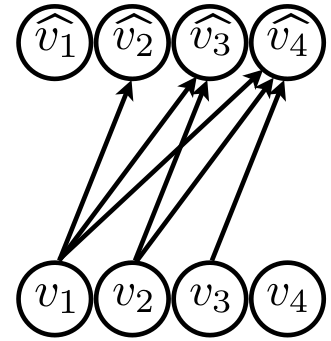
\includegraphics[scale=0.25]{chap3-img/FVSBN}
			\caption{مدل FVBN}
			\label{chap3-fig2-1}
		\end{subfigure}		
		\begin{subfigure}{0.4\textwidth}
			\centering
			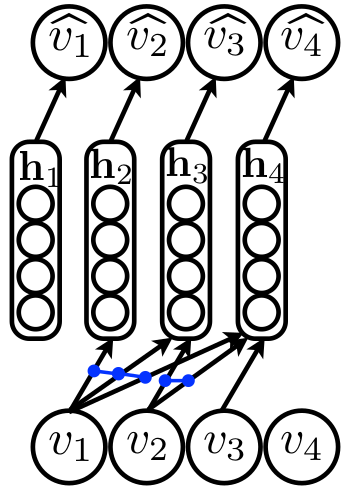
\includegraphics[scale=0.25]{chap3-img/NADE}
			\caption{مدل NADE}
			\label{chap3-fig2-2}
		\end{subfigure}
		\caption{مدل‌های FVBN و NADE
			\cite{larochelle2011neural} }
		\label{chap3-fig2}
	\end{figure}


\section{روش‌های مدل‌سازی موضوعی}
\label{chap3sec3}
همان‌طور که پیش از این در بخش
\ref{chap2sec12}
بیان کردیم روش‌های مدل‌سازی موضوع به مدل‌هایی گفته می‌‌شود که یک چکیده از موضوعات موجود در یک سند یا مجمومه‌ای از اسناد را تشخیص داده و استخرج می‌‌کنند. این مدل‌ها را می‌‌توان در دو دسته‌ی کلی‌ شامل مدل‌های گرافی که بر پایه‌ی قوانین احتمالاتی و رابطه‌‌ی بیز هستند و همچنین مدل‌های شبکه‌های عصبی تقسیم‌بندی کرد. در ادامه ضمن معرفی هر کدام از این کلاس‌ها با مهمترین مدل‌های موجود در این حوضه آشنا می‌‌گردیم.
	\subsection{مدل تکرار عبارت-معکوس تکرار سند}
	\label{chap3sec3sub1}
	 تاکنون محققین حوضه‌ی بازیابی اطلاعات پیشرفت‌های قابل توجهی‌ در زمینه‌ی مدل کردن مجموعه‌ی اسناد یا هر مجموعه‌ی گسسته‌ از داده‌ها داشته‌اند
	\cite{baeza1999modern}.
	در روش پایه که توسط پژوهشگران حوزه‌ی
	IR
	پیشنهاد گردیده و امروزه همچنان در مرورگر‌های اینترنتی مورد استفاده قرار می‌‌گیرد، هر سند متنی از یک مجموعه اسناد به یک بردار اعدد حقیقی‌ تبدیل می‌شود که شامل نسبت‌های تعداد تکرار کلمات مختلف است.
	
	 در این روش که به آن تکرار عبارت-معکوس تکرار سند\LTRfootnote{Term Frequency-Inverse Document Frequency} 
	($tf-idf$) \cite{salton1986introduction}
	گفته می‌شود و در سال 1986 توسط
	Salton
	معرفی شد یک لغات‌نامه از تمام کلمات متمایز ساخته می‌‌شود، سپس برای هر سند در مجموعه‌ی اسناد تعداد رخداد تمام کلمات متمایز محاسبه می‌‌شود. پس از نرمال‌سازی مناسب (بیشتر در مقیاس لگاریتمی) مقادیر بدست آماده برای هر کلمه، هر مقدار بر معکوس تعداد سندهای شامل آن کلمه در کّل مجموعه‌ی اسناد تقسیم می‌‌گردد. مقادیر نهایی بدست آماده برای هر کلمه که به آن مقادیر
	$tf-idf$
	گفته می‌شود به صورت یک بردار ستونی در یک ماتریس جایگذاری می‌شوند. بنابراین در روش
	$tf-idf$
	یک مجموعه سند به ماتریسی
	$m \times n$
	تبدیل می‌شود که در آن
	$m$
	تعداد کلمات متمایز در مجموعه سند و
	$n$
	تعداد سندهای موجود در مجموعه سند هستند.
	
	به عنوان مثال یک مجموعه اسناد که تنها از دو سند تشکیل شده است را در نظر بگیرید. اگر جدول تکرار کلمه‌ها برای هر سند مانند شکل
	\ref{chap3-fig3}
	باشد، آنگاه محاسبه‌ی
	$tf-idf$
	برای یک کلمه مانند
	$"this"$
	به صورت زیر است:
\begin{flushleft}
$Document_1:\  tf("this",d_1) = \dfrac{1}{5} = 0.2 \qquad Document_2:\  tf("this",d_2) = \dfrac{1}{7} \approx 0.14$

$idf("this",D) = \log(\dfrac{2}{2}) = 0$

$Document_1:\  tfidf("this",d_1) = 0.2 \times 0 = 0 \qquad Document_2:\  tfidf("this",d_2) = 0.14 \times 0 = 0$
\end{flushleft}
صفر شدن مقدار 
$tf-idf$ 
برای 
$"this"$ 
نشان می‌‌دهد که این کلمه از آنجا که در تمام سند‌ها تکرار شده است بنابراین از اهمیت کمی‌ برخوردار است.   
	\begin{figure}[b]
		\centering
		\begin{subfigure}{0.3\textwidth}
			\centering
			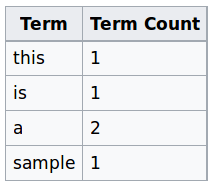
\includegraphics[scale=0.4]{chap3-img/tf-idf1}
			\caption{سند اول}
			\label{chap3-fig3-1}
		\end{subfigure}		
		\begin{subfigure}{0.3\textwidth}
			\centering
			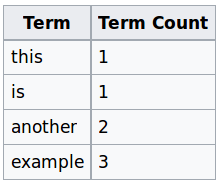
\includegraphics[scale=0.4]{chap3-img/tf-idf2}
			\caption{سند دوم}
			\label{chap3-fig3-2}
		\end{subfigure}
		\caption{جدول‌های تعداد تکرار کلمات برای یک مجموعه‌ی اسناد ۲ سندی}
		\label{chap3-fig3}
	\end{figure}
	
	\subsection{مدل فهرست‌سازی معنایی نهفته}
	\label{chap3sec3sub2}
	علی‌رغم ویژگی‌‌های مناسب مدل کاهش‌دهنده‌ی
	$tf-idf$
	مانند شناسایی مجموعه کلمه‌هایی که برای هر سند آن را از دیگر سند‌ها در یک مجموعه متمایز می‌‌کند، مشکلاتی مانند میزان کاهش ناچیز طول هر سند و همچنین در نظر نگرفتن خصوصیت آماری‌ در داخل هر سند از نقاط ضعف این روش است. برای غلبه بر این مشکلات محققین حوزه‌ی
	IR
	چندین مدل کاهش بعد دیگر معرفی‌ کردند که مهمترین آن‌ها مدل فهرست کردن معنایی نهفته\LTRfootnote{Latent Semantic Indexing}
	(LSI)
	است که توسط
	Deerwester \cite{deerwester1990indexing}
	 و همکاران در سال 1990 ارائه گردید.
	
	مدل
	LSI
	با استفاده از تجزیه مقدار منفرد\LTRfootnote{Singular Value Decomposition}
	 بر روی ماتریس خروجی از مدل
	$tf-idf$
	یک زیرفضای خطی\LTRfootnote{Linear Subspace}
	‌ در فضای ویژگی‌‌های مدل
	$tf-idf$
	شناسایی می‌‌کند. این روش منجر به کاهش و فشرده‌سازی قابل توجهی‌ در مجموعه‌های بزرگ می‌‌گردد. همچنین
	Deerwester
	و همکاران ادعا کردند که ویژگی‌‌های بدست آماده توسط مدل
	LSI
	که در حقیقت یک ترکیب خطی‌ از ویژگی‌‌های مدل
	$tf-idf$
	می‌باشند، توانایی تشخیص بعضی‌ از ویژگی‌‌های زبانی مانند مترادف و متضاد را دارند
	\cite{deerwester1990indexing}.
	
	\subsection{مدل فهرست‌سازی معنایی نهفته‌ی احتمالاتی}
	\label{chap3sec3sub3}
	برای اثبات ادعا‌های مطرح شده توسط مدل
	LSI (بخش \ref{chap3sec3sub2})
	و همچنین بررسی‌ نقاط ضعف و قدرت این مدل، روش فهرست‌سازی معنایی نهفته‌ی احتمالاتی\LTRfootnote{probabilistic Latent Semantic Indexing} (pLSI)
	 توسط 
	Hofmann \cite{hofmann1999probabilistic}
در سال 1999 معرفی شد. مدل 
	pLSI
	یک مدل مولد احتمالاتی است که از آن به عنوان یک مدل موضوعی نیز یاد می‌شود
	\cite{blei2003latent}.
	 در روش 
	 pLSI
	 هر کلمه‌ی داخل هر سند به عنوان یک نمونه از یک مدل مخلوط مدل می‌شود
	 \cite{hofmann1999probabilistic}.
	  مؤلفه‌های این مدل مخلوط در واقع متغیرهای تصادفی چندجمله‌ای می‌باشند که می‌توان آن‌ها را به عنوان یک نمایش از موضوع‌های موجود در سند دانست. بنابراین هر کلمه از یک موضوع خاص تولید می‌‌شود و کلمه‌های مختلف در داخل یک سند ممکن است از موضوع‌های مختلفی‌ تولید شوند. در نتیجه هر سند به صورت لیستی از این توزیع‌های مخلوط نمایش داده می‌‌شود و در واقع هر سند به یک مجموعه‌ی از پیش تعیین شده از نظر تعداد از توزیع‌های احتمالاتی کاهش پیدا می‌کند.
	
	در شکل
	\ref{chap3-fig4}
	مدل
	pLSI
	را مشاهده می‌کنید‌. در شکل
	\ref{chap3-fig4}
	 مجموعه سند دارای
	M
	سند مختلف است که هر کدام از آن‌ها دارای
	N
	کلمه‌ هستند.همچنین در این شکل
	(\ref{chap3-fig4})، $w$
	نشان دهنده‌ي کلمه، و
	$z$
	نماد یک توزیع چندجمله‌ای از موضوع‌ها در یک سند مشخص است. با توجه به شکل
	\ref{chap3-fig4}
	و توضیحات بیان شده، در مدل
	pLSI
	فرض بر آن است که یک سند مانند
	$d$
	و یک کلمه‌ مانند
	$w_n$
	در صورت داشتن یک موضوع مشاهده نشده مانند
	$z$
	همان‌طور که در رابطه‌ی
	\begin{align}
		\centering
		\label{chap3-eq5}
		p(d,w_n) = p(d) \sum_{z} p(w_n|z)p(z|d)
	\end{align}
	مشاهده می‌‌شود دارای استقلال شرطی از یکدیگر هستند.

	همان‌طور که پیش از این در بخش
	\ref{chap2sec12}
	بیان شد، یک فرض اساسی‌ که مدل‌های موضوعی بر اساس آن ساخته می‌‌شوند در نظر گرفتن چند موضوع برای هر سند است. مدل
	pLSI
	به عنوان یک مدل موضوعی این امکان را در رابطه‌ی
	\ref{chap3-eq5}
	برای یک سند مشخص مانند
	$d$
	با ترم
	$p(z|d)$
	در نظر می‌‌گیرد. توجه شود که در اینجا برچسب
	$d$
	یک برچسب ساختگی برای سند‌های مجموعه داده‌ی آموزش است، در حقیقت
	$d$
	یک متغیر تصادفی چندجمله‌ای است که مقادیر ممکن برای آن برابر با تعداد سند‌های موجود در مجموعه داده‌ی آموزش که مدل در آن
	$p(z|d)$
	را یاد می‌‌گیرد، است. به همین دلیل مدل
	pLSI
	یک مدل مولد مناسب برای اسناد‌ ناست، چرا که هیچ راهی‌ برای تقابل و تخصیص احتمال به موضوع‌هایی که آن‌ها را در داده‌های آموزش مشاهده 
	نکرده است در این مدل وجود ندارد
	\cite{blei2003latent}.
	
	مشکل دیگر مدل
	pLSI
	بدلیل استفاده از توزیع‌های احتمالی‌ موجود در داده‌های آموزش است که باعث می‌‌شود پارامترهایی که باید توسط مدل تخمین زده شوند به صورت خطی با اندازه داده‌های آموزش رشد پیدا کنند
	\cite{blei2003latent}.
	\begin{figure}
		\centering
		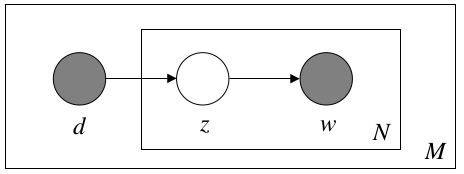
\includegraphics[scale=0.4]{chap3-img/pLSI}
		\caption{مدل فهرست‌ساری معنایی نهفته‌ی احتمالاتی \cite{blei2003latent}}
		\label{chap3-fig4}
	\end{figure}
	
	
	\subsection{مدل تخصیص دیریکله‌ی پنهان}
	\label{chap3sec3sub4}
	مدل تخصیص دیریکله‌ی پنهان 
\LTRfootnote{Latent Dirichlet Allocation}	(LDA)
	یک مدل احتمالاتی مولد گرافی است که در سال 2003 توسط 
	Blei 
	و همکاران
	\cite{blei2003latent}
	معرفی شد و پس از آن به عنوان پایه و اساس مدل‌سازی موضوع در بخش روش‌های گرافی‌ قرار گرفت. مدل
	LDA
	 را می‌‌توان معروف‌ترین و مهم‌ترین روش مدل‌سازی موضوع در بخش مدل‌های گرافی‌ و مدل‌های بیزی دانست. تا به امروز روش‌های بسیاری از این مدل برای کاربرد‌های مختلف مشتق شده‌اند که در بخش‌های
	 \ref{chap3sec4sub1}
	 و
	 \ref{chap3sec4sub2}
	 دو مورد از آن‌ها را که به تشخیص همزمان موضوع و احساس از داده‌های متنی می‌‌پردازند را بررسی‌ می‌‌کنیم.
	 
	 
	 
	 در روش  
	LDA
	مانند دیگر روش‌های مدل‌سازی موضوع، هر سند متنی به صورت یک توزیع مخلوط بر روی موضوع‌های مختلف‌ که در آن هر موضوع به وسیله‌ی یک توزیع بر روی کلمه‌ها مشخص می‌‌شود در نظر گرفته می‌شود
	\cite{blei2003latent}.
	شکل
	\ref{chap3-fig5}
	مدل
	LDA
	استاندارد را نشان می‌‌دهد.	
	
همان‌طور که در بخش
\ref{chap3sec3sub3}
بیان شد مدل
pLSI
از مشکلاتی مانند بزرگ شدن فضای پارامترهای مساله به صورت خطی‌ با اندازه داده ‌های آموزش و همچنین عدم توانایی در تخصیص احتمال به موضوع‌ها و سند‌های از پیش دیده نشده رنج می‌‌برد. مدل
LDA
با در نظر گرفتن وزن‌های توزیع مخلوط موضوع‌ها به عنوان یک متغیر تصادفی پنهان، به جای یک مجموعه بزرگ از پارامترهای منحصر به فرد که 
مستقیما به داده‌های آموزش متصل باشند بر این دو مشکل غلبه کرده است.
	\begin{figure}[!t]
		\centering
		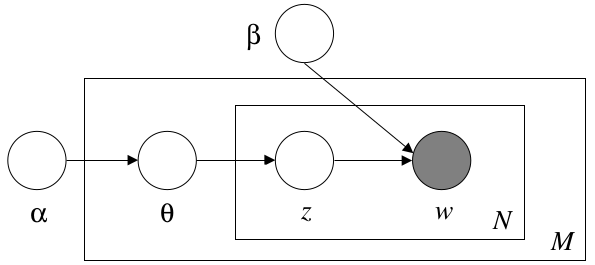
\includegraphics[scale=0.4]{chap3-img/LDA}
		\caption{مدل تخصیص دیریکله‌ی پنهان \cite{blei2003latent}}
		\label{chap3-fig5}
	\end{figure}

در مدل
LDA
که در شکل
\ref{chap3-fig5}
نشان داده شده است،
$\beta$
یک ماتریس دو بعدی احتمالاتی با اندازه
$k \times V$
 است که در آن
$k$
برابر با تعداد موضوع‌ها و
$V$
برابر با اندازه لغت‌نامه‌ یا تعداد کلمات متمایز در متن است. درایه‌های این ماتریس، احتمال حضور هر کلمه در هر موضوع را نشان می‌‌دهند. برای مثال
$\beta_{ij}$
نشان دهنده‌ی احتمال حضور کلمه‌ی
$j$ام
 در موضوع
$i$ام
 است. همان‌طور که در بخش
\ref{chap2sec4}
در مورد مدل‌های گرافی توضیح داده شده در شکل
\ref{chap3-fig5}
پارامتر‌های
$\beta,\ \alpha,\ \theta ,\ z$
متغیر‌های پنهان هستند و
$w$
تنها متغیر قابل مشاهده در مدل
LDA
می‌ باشد.

در مدل
LDA
پارامتر
$\alpha$
یک بردار
$k$
بعدی که
$k$
تعداد موضوع‌ها را نشان می‌دهد، است.
$\alpha$
احتمال اولیه‌ی یک توزیع دیریکله است که با نمونه گرفتن از آن با استفاده از رابطه‌ی
\begin{align}
	\centering
	\label{chap3-eq6}
	p(\theta|\alpha) = \dfrac{\Gamma (\sum_{i=1}^{k} \alpha_i)}{\prod_{i=1}^{k} \Gamma(\alpha_i)} \theta_1^{\alpha_1 -1}\ ...\ \theta_k^{\alpha_k -1}
\end{align}
به ازای هر سند بردار
$\theta$
که یک توزیع چندجمله‌ای است و نشان دهنده‌ی توزیع موضوع‌ها در هر سند است را بدست می‌‌آوریم. در رابطه‌ی
\ref{chap3-eq6}، $\Gamma$
تابع گاما است که در بخش
\ref{chap2sec8}
آن را معرفی‌ کردیم.


با داشتن
$\alpha$
و
$\beta$
توزیع مشترک پارامترهای
$\theta$، $\textbf{z}$
و
$\textbf{w}$
از رابطه‌ی
\begin{align}
	\centering
	\label{chap3-eq7}
	p(\theta,\textbf{z},\textbf{w}|\alpha,\beta) = p(\theta|\alpha)\prod_{n=1}^{N}p(z_n|\theta)p(w_n|z_n,\beta)
\end{align}
بدست می‌‌آید. در رابطه‌ی
\ref{chap3-eq7}، $\theta$
یک توزیع چندجمله‌ا‌ی موضوعی، بردار
$\textbf{z}$
یک مجموعه
$N$تایی
‌ از موضوع‌ها که از
$\theta$
نمونه گرفته می‌‌شود و
$\textbf{w}$
یک مجموعه
$N$
تائی‌ از کلمه‌ها که مشروط به
$\beta$
و
$z$
نمونه گرفته می‌‌شود. در ادامه با انتگرال‌گیری روی
$\theta$
و سیگما روی
$z$
 احتمال حاشیه‌ای برای یک سند به فرم رابطه‌ی
\begin{align}
	\centering
	\label{chap3-eq8}
	p(\textbf{w}|\alpha,\beta) = \int p(\theta|\alpha) \left( \prod_{n=1}^{N} \sum_{z_n}p(z_n|\theta)p(w_n|z_n,\beta) \right)   d\theta
\end{align}
  بدست می‌‌آید. و در نهایت با ضرب احتمال‌های حاشیه‌ای برای هر سند احتمال یک مجموعه سند به شکل رابطه‌‌ی
\begin{align}
	\centering
	\label{chap3-eq9}
	p(D|\alpha,\beta) =\prod_{d=1}^{M} \int p(\theta|\alpha) \left( \prod_{n=1}^{N} \sum_{z_n}p(z_n|\theta)p(w_n|z_n,\beta) \right)d\theta_d
\end{align}
  بدست می‌‌آید.

برای استنتاج در مدل
LDA
نمی‌توان از روش‌های مستقیم استفاده کرد و به جای آن باید از روش‌های تقریبی مانند، تقریب لاپلاس\LTRfootnote{Laplace Approximation}،
 تقریب تغییراتی\LTRfootnote{Variational Approximation}
 ‌ و یا روش
MCMC
که در بخش
\ref{chap2sec6}
معرفی‌ شد استفاده کرد. در مدل معرفی‌ شده توسط آقای
Blei
همکاران 
\cite{blei2003latent}
در سال ۲۰۰۳ از روش تقریب تغییراتی‌ برای استنتاج در مدل
LDA
استفاده شده است. شکل
\ref{chap3-fig11}
خروجی مدل
LDA
برای چهار موضوع مختلف به همراه کلماتشان در یک متن نمونه را نشان می‌‌دهد.

	\begin{figure}[!t]
		\centering
		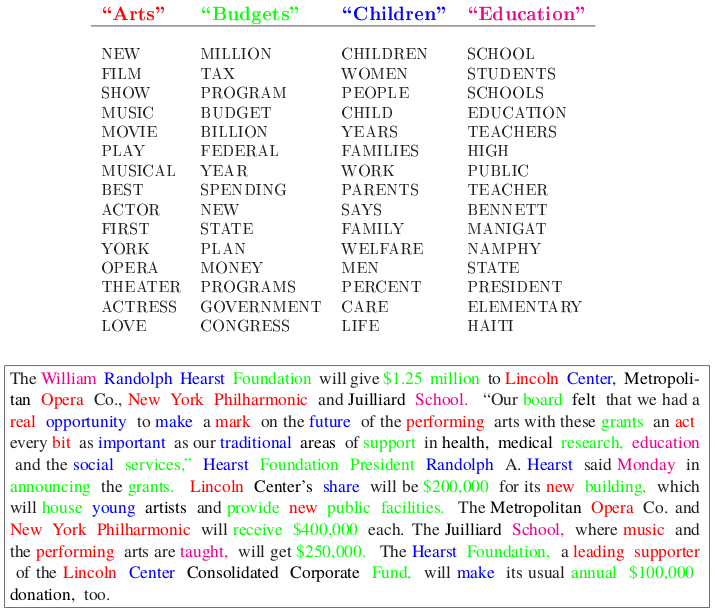
\includegraphics[scale=0.4]{chap3-img/LDAexample}
		\caption{نمونه خروجی مدل LDA برای چهار موضوع مختلف \cite{blei2003latent}}
		\label{chap3-fig11}
	\end{figure}



	\subsection{مدل Softmax تکرارشده}
	\label{chap3sec3sub5}
	
	مدل
	Softmax
	تکرارشده\footnote{Replicated Softmax}
	(RS)
	که در سال ۲۰۰۹ توسط
	Hinton
	و
	Salakhutdinov \cite{hinton2009replicated}
	معرفی‌ شد، اولین روش مدل‌سازی موضوع بر پایه‌ی شبکه‌های عصبی است.
	RS
	گسترش‌یافته‌ی مدل
	RBM
	است که از آن برای تشخیص توزیع موضوع‌های مختلف در داده‌های متنی استفاده می‌‌شود. مدل
	RBM
	به دلیل محدودیت‌هایی مانند محدود بودن به بردار ورودی باینری و در نظر گرفتن طول ثابت برای وروی‌ها نمی‌‌تواند در تشخیص توزیع موضوع مورد استفاده قرار بگیرد، چرا که اولا کلمات باینری نیستند و دوما در یک مجموعه از داده‌های متنی طول اسناد با یکدیگر متفاوت هستند
	\cite{hinton2009replicated}.
	
	در شکل
	\ref{chap3-fig6}
	مدل
	RS
	نشان داده شده است. همان‌طور که در شکل
	\ref{chap3-fig6}
	مشاهده می‌‌شود مدل
	RS
	مانند مدل
RBM
	دارای یک ساختار دو بخشی متشکل از یک لایه‌ی قابل مشاهده و یک لایه‌ی پنهان است. در مدل
	RS
	نیز مانند مدل
	RBM
	یک تابع انرژی وابسته به سند ورودی و بردار پنهان آن به شکل رابطه‌ی
	\begin{align}
		\centering
		\label{chap3-eq10}
		E(\textbf{V},\textbf{h}) = -\sum_{j=1}^{F} \sum_{k=1}^{K} W_j^k h_j \hat{v}^k - \sum_{k=1}^K \hat{v}^k b^k -D\sum_{j=1}^F h_ja_j
	\end{align}
	تعریف می‌‌شود که ضمن کمینه کردن آن توزیع موضوع‌های مختلف در متن توسط مدل یاد گرفته می‌‌شود. احتمال مشاهده‌ی هر سند ورودی در این مدل به کمک رابطه‌ی
	\begin{align}
		\centering
		\label{chap3-eq11}
		p(\textbf{V}) = \dfrac{1}{Z}\sum_{h}exp(-E(\textbf{V},\textbf{h}))
	\end{align}
	محاسبه می‌‌گردد که در آن
	$Z$
	همانند مدل
	RBM
	تابع قسمت‌بندی است و از رابطه‌ی
	\begin{align}
		\centering
		\label{chap3-eq12}
		Z = \sum_{V}\sum_{h}exp(-E(\textbf{V},\textbf{h}))
	\end{align}
	بدست می‌‌آید.
	\begin{figure}[!t]
		\centering
		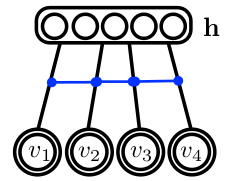
\includegraphics[scale=0.4]{chap3-img/RS}
		\caption{مدل Softmax تکرارشده \cite{hinton2009replicated}}
		\label{chap3-fig6}
	\end{figure}	
	در رابطه‌ی
	\ref{chap3-eq10}, D
	اندازه سند ورودی،
	$W$
	ماتریس وزن بین لایه‌ی قابل مشاهده و لایه‌ی پنهان،
	$\textbf{b}$
	و
	$\textbf{a}$
	به ترتیب بردار بایاس لایه‌های قابل مشاهده و پنهان هستند. همچنین
	$\hat{v}^k$
	که آن را به صورت
	$\hat{v}^k = \sum_{i=1}^{D} v_i^k$
	 تعریف می‌‌کنیم برابر با تعداد
	$k$امین 
	کلمه‌ی لغت‌نامه است. در مدل
		RS
	نیز مانند مدل
	RBM
	برای آموزش از الگوریتم
	CD
	که در بخش
	\ref{chap2sec7}
	معرفی شد استفاده می‌‌شود.
		 
	\subsection{مدل شبکه‌‌ی عصبی خود رگرسیو تخمین‌زننده‌ی توزیع سندی}
	\label{chap3sec3sub6}
مدل شبکه‌‌ی عصبی خود رگرسیو تخمین‌زننده‌ی توزیع سندی
\LTRfootnote{Document Neural Autoregressive Distribution Estimator}
(DocNADE)
که در شکل
\ref{chap3-fig7}
مشاهده می‌‌شود یک روش بدون‌نظارت برای مدل‌سازی موضوع بر پایه‌ی شبکه‌های عصبی است. این مدل در سال ۲۰۱۲ توسط
Larochelle
و
Lauly \cite{larochelle2012neural}
با ترکیب مدل‌های
NADE
و
RS
معرفی‌ شد.

 بردار ورودی در این مدل بر خلاف مدل
NADE
که در آن بردار ورودی می‌‌بایست حتما باینری باشد، یک بردار چندجمله‌ای به شکل بردار ورودی در مدل
RS
است. اما در این مدل مانند مدل
NADE
احتمال هر کلمه در داخل سند به شرط تمام کلمات قبل از آن بدست می‌‌آید
\cite{larochelle2012neural}.
 تفاوت دیگر مدل
DocNADE
با مدل
NADE
در نحوه‌ی بدست آوردن احتمال مشاهده‌ی هر کلمه به شرط کلمات قبل است. در مدل
DocNADE
احتمال در لایه‌ی نهایی با استفاده از یک ساختار درختی محاسبه می‌‌گردد. در درخت مورد نظر که در شکل
\ref{chap3-fig7}
مشخص شده تمام کلمات در برگ‌های آن قرار می‌‌گیرند و هر مسیر از ریشه تا برگ برابر با احتمال مشاهده‌ی ‌کلمه‌ی متناظر با آن است. استفاده از یک چنین ساختار درختی موجب می‌‌گردد تا بدست آوردن احتمال هر کلمه نسبت به اندازه لغت‌نامه مقداری لگاریتمی داشته باشد که در کاربرد‌های عملی‌ بسیار کارآمدتر از حالت مستقیم که خطی‌ است است
\cite{larochelle2012neural}.

رابطه‌های
\begin{align}
	\centering
	\textbf{h}_i(\textbf{v}_{<i}) = sigm(\textbf{c}+\sum_{k<i}\textbf{W}_{:,v_k})
	\label{chap3-eq13}
\end{align}
و
\begin{align}
	\centering
	p(v_i=w|\textbf{v}_{<i}) = \frac{exp(b_w +\textbf{V}_{w,:}\textbf{h}_i(\textbf{v}_{<i})}{\sum_{w'}exp(b_{w'}+\textbf{V}_{w',:}\textbf{h}_i(\textbf{v}_{<i})}
	\label{chap3-eq14}
\end{align}
به ترتیب نحوه‌ی به دست آوردن مقادیر لایه‌ی پنهان و احتمال مشاهده‌ی هر کلمه به شرط تمام کلمات پیشین در مدل
DocNADE
 را نشان می‌‌دهند. در جدول
\ref{chap3-tb1}
نمونه‌ای از چهار موضوع یاد گرفته شده توسط مدل
DocNADE
به همراه ده کلمه‌ای‌ که در هر موضوع بیشترین احتمال را داشته‌اند مشاهده می‌شود.

  \begin{figure}[!t]
  	\centering
  	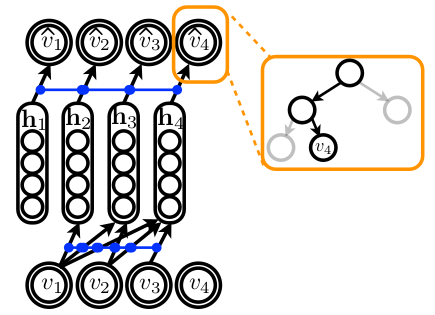
\includegraphics[scale=0.4]{chap3-img/DocNADE}
  	\caption{مدل شبکه‌‌ی عصبی خود رگرسیو تخمین‌زننده‌ی توزیع سندی \cite{larochelle2012neural}}
  	\label{chap3-fig7}
  \end{figure}

\section{مدل‌های مشترک موضوع و احساس}
تمام مدل‌های بررسی‌ شده در بخش‌های پیشین تنها توانایی تشخیص موضوع از داده‌های متنی را داشتند. گروه دیگری از مدل‌های موضوعی وجود دارند که به صورت همزمان به تشخیص موضوع‌ها و احساس همراه با هرکدام می‌‌پردازند. در بخش های
\ref{chap3sec4sub1}
و
\ref{chap3sec4sub2}
دو مدل موجود در این زمینه، که یکی‌ به تشخیص موضوع و احساس آن در سطح کلمه
(\ref{chap3sec4sub1})
 و یکی‌ در سطح جمله
(\ref{chap3sec4sub2})
  می‌‌پردازد را بررسی‌ می‌‌کنیم. همچنین در بخش
\ref{chap3sec4sub3}
  یک مدل با رویکردی نظارت شده که به تازگی برای تشخیص موضوع و احساس در داده‌های متنی پیشنهاد شده است را معرفی‌ می‌‌کنیم.
  \begin{table}[!b]
	\centering
	\begin{tabular}{|c|c|c|c|}
		\hline
		\multicolumn{4}{|c|}{چهار موضوع بادگرفته شده توسط DocNADE}\\
		\hline
		card 	 & shuttle 		& team 	   & christianity\\
		driver 	 & orbit 		& games    & god\\
		drivers  & lunar 		& seasons  & pgp\\ 
		bus		 & spacecraft 	& baseball & jesus\\ 
		video	 & nasa  		& players  & bible\\ 
		vga		 & space 		& game     & faith\\ 
		monitor  & launch 		& hockey   & muslim\\ 
		ibm   	 & saturn  		& play 	   & christ\\ 
		cards	 & billion		& teams    & atheist\\
		ram    	 & satellite	& sale     & christians\\
		\hline
	\end{tabular}
	\caption{نمومه‌ای از موضوع‌های یادگرفته شده توسط مدل DocNADE \cite{larochelle2012neural}}
	\label{chap3-tb1}
\end{table}

	\subsection{مدل یکی‌سازی احساس-موضوع}
	\label{chap3sec4sub2}
	
	پیدا کردن جنبه‌هایی از یک محصول که کاربران در بازبینی‌های آنلاین خود مورد ارزیابی قرار می‌‌دهند همواره کار مشکلی‌ بوده است. علاوه بر تشخیص موضوع‌ها و جنبه‌های موجود در یک بازبینی آنلاین، تشخیص احساس همراه با هر کدام نیز برای شرکت سازنده و افراد دیگری که به دنبال کسب اطلاعات در مورد یک محصول خاص هستند، اهمیت دارد. مدل یکی‌سازی احساس-موضوع
\LTRfootnote{Aspect and Sentiment Unification Model}
	(ASUM)
	در سال ۲۰۱۱ برای تشخیص موضوع‌ها و احساس همراه با آن‌ها در بازبینی‌های آنلاین توسط
	Jo
	و
	Oh
	معرفی‌ شد
	\cite{jo2011aspect}.
	
	شکل
	\ref{chap3-fig9}
	مدل
	ASUM
	را نشان می‌‌دهد. این مدل همان‌طور که در شکل
	\ref{chap3-fig9}
	مشاهده می‌‌گردد گسترش یافته‌ی مدل
	LDA
	است
	\cite{jo2011aspect}
	و در گروه مدل‌های احتمالاتی گرافی‌ مولد قرار می‌‌گیرد. در مدل
	LDA
	هر کلمه به صورت مجزا از یک موضوع نمونه گرفته می‌‌شود و فرض بر آن است که هر کلمه می‌‌تواند موضوع خود را داشته باشد، اما در مدل
	ASUM
	فرض بر آن است که هر جمله دارای یک موضوع است و تمام کلمات یک جمله از یک موضوع نمونه گرفته می‌‌شوند
	\cite{jo2011aspect}.
	
در مدل
ASUM
ما برای هر سند یک توزیع چندجمله‌ای احساسی‌ و برای هر یک از احساس‌ها یک توزیع چندجمله‌ای موضوعی داریم. در حالت مولد پس از نمونه گرفتن از توزیع احساسی‌ و توزیع موضوعی متناسب با احساس انتخاب شده برای سند جاری، برای هر جمله یک احساس و یک موضوع نمونه گرفته ‌می‌‌شود و سپس تمام کلمات آن جمله از آن موضوع و احساس تولید می‌‌شوند
\cite{jo2011aspect}.

\begin{figure}[!t]
	\centering
	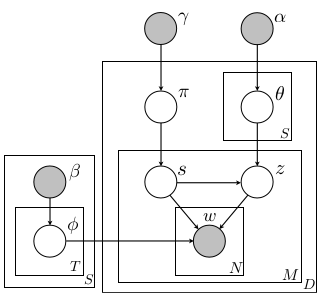
\includegraphics[scale=0.5]{chap3-img/ASUM}
	\caption{مدل یکی‌سازی احساس-موضوع \cite{jo2011aspect}}
	\label{chap3-fig9}
\end{figure}


	\subsection{مدل نظارت‌شده‌ی ضعیف تشخیص مشترک احساس-موضوع}
	\label{chap3sec4sub1}
مدل نظارت‌شده‌ی ضعیف تشخیص مشترک احساس/موضوع
(JST) \cite{lin2012weakly}
 که در شکل 
\ref{chap3-fig8}
مشاهده می‌‌شود در سال ۲۰۱۲ توسط
 Lin
 و همکاران معرفی‌ شد. مدل
 JST
  همانند 
 LDA
 یک مدل احتمالاتی مولد گرافی است. در واقع
 JST
 گسترش یافته‌ی‌ مدل 
 LDA
 است که علاوه بر تشخیص موضوع به تشخیص احساس از داده‌های متنی نیز می‌پردازد.  خاصیت نظارت‌شده‌ی ضعیف باعث می‌‌شود که در مقایسه با سایر مدل‌ها
 ، JST
  به راحتی‌ قابل انتقال به یک دامنه‌ی دیگر بدون کاهش محسوس در کارایی که در سایر مدل ها این اتفاق رخ می‌‌دهد باشد. از دیگر تفاوت‌های مدل
   JST
    با سایر مدل‌ها این است که تمام مدل‌های موجود به تشخیص احساس کلی‌ متن می‌پردازند، این در حالی‌ است که
     JST
      به تشخیص احساس همراه با هر موضوع و احساس کلی‌ متن می‌‌پردازد که در مسائل پیش‌رو دید بهتری را به کاربر خواهد داد.
 
  برای مدل کردن احساس در 
 JST
 یک لایه بین سند و موضوع اضافه می‌شود. با وجود این، 
 JST
 یک مدل چهار لایه است که در آن اسناد با احساسات همراه هستند و احساسات با موضوع‌ها همراه هستند و در نهایت کلمات با هردو برچسب احساس و موضوع همراه هستند
 \cite{lin2012weakly}.
 
  فرض کنید که یک مجموعه سند در اختیار داریم که شامل
  D
   سند است که به صورت  
  $C = \{d_1,\ ...,d_D\}$
   مشخص می‌‌شوند، هر سند موجود دنباله‌ای از  
  $N_d$
   کلمه است که با  
   $d=\{w_1,\ ...,w_{N_d} \}$
    مشخص می‌‌شوند و هر کلمه در داخل سند یک مورد از 
    V
    کلمه‌ی مجزای واژگان است که به صورت 
    $\{1,\ ...,V\}$
    شاخص‌گذاری شده‌اند. همچنین 
    S
    تعداد برچسب‌های احساس متمایز است و 
    T
    برابر است با تعداد کلی‌ موضوع‌ها.
    
     روند تولید کلمه‌ی  
   $w_j$
    در سند 
    d
    تحت مدل 
    JST
    شامل سه‌ مرحله می‌‌شود. ابتدا یک برچسب احساس مثلا  
    $l$
    از  
    $\pi_d$
    که توزیع احتمالاتی احساس برای هر سند است انتخاب شده، سپس با توجه به برچسب احساس انتخاب شده و مشروط به آن یک موضوع از توزیع موضوعی 
    $\theta_{d,l}$
     نمونه گرفته می‌شود. در نهایت با داشتن برچسب موضوع واحساس، ازتوزیع احتمالاتی مشروط به موضوع و احساس برای هر مجموعه سند یک کلمه تولید می‌شود. 
   	\begin{figure}[!h]
   		\centering
   		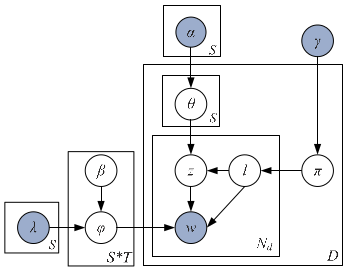
\includegraphics[scale=0.5]{chap3-img/JST}
   		\caption{مدل نظارت‌شده‌ی ضعیف تشخیص مشترک احساس/موضوع \cite{lin2012weakly}}
   		\label{chap3-fig8}
   	\end{figure}
    
     لازم به ذکر است که در مدل 
     LDA
به ازای هر سند یک توزیع احتمالاتی برای موضوع‌ها وجود دارد، اما در مدل 
     JST
     به ازای هر برچسب احساس یک توزیع احتمالاتی برای موضوع‌ها در سند تعریف می‌شود. به طور مثال اگر سه‌ برچسب احساس مثبت، منفی‌ یا بی‌طرف در نظر گرفته شود، برای هر سند سه‌ توزیع احتمالاتی وجود خواهد داشت که هر کدام متناظر با یک احساس خواهند بود. تفاوت دیگری که بین مدل
LDA
       و
JST
است از این قرار است که در
LDA
  به هنگام نمونه‌برداری از کلمه، این کار تنها مشروط به توزیع موضوعی برای مجموعه سند انجام می‌‌شود ولی‌ در
JST
    این نمونه برداری مشروط به هر دو توزیع موضوعی و احساسی‌ انجام می‌‌شود
    \cite{lin2012weakly}.
    در شکل
    \ref{chap3-fig12}
    می‌ توان خروجی مدل
    JST
    برای دو احساس مثبت 
    \ref{chap3-fig12-1}
    و منفی
    \ref{chap3-fig12-2}
    ‌  به همراه دو موضوع برای هر احساس و همچنین پانزده کلمه‌ای که بیشترین احتمال در هر موضوع داشتند را مشاهده می‌‌کنید.
    
	\begin{figure}[!b]
		\centering
		\begin{subfigure}{0.4\textwidth}
			\centering
			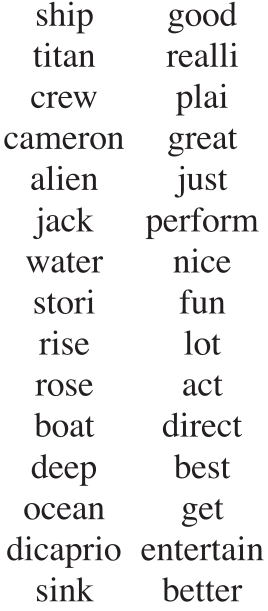
\includegraphics[scale=0.2]{chap3-img/JSTexamplep}
			\caption{نمونه خروجی مدل JST برای احساس مثبت}
			\label{chap3-fig12-1}
		\end{subfigure}		
		\begin{subfigure}{0.4\textwidth}
			\centering
			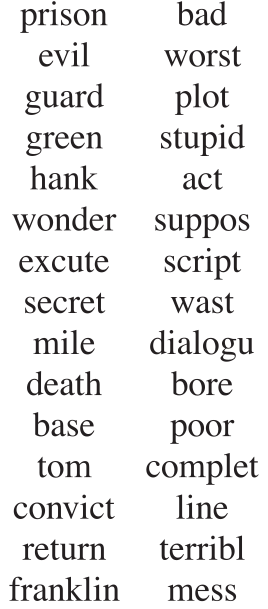
\includegraphics[scale=0.2]{chap3-img/JSTexamplen}
			\caption{نمونه خروجی مدل JST برای احساس منفی}
			\label{chap3-fig12-2}
		\end{subfigure}
		\caption{خروجی مدل JST برای دو احساس مثبت و منفی‌ و دو موضوع برای هر احساس و پانزده کلمه در هر موضوع \cite{lin2012weakly}}
		\label{chap3-fig12}
	\end{figure}

\subsection{مدل نظارت‌شده‌ی مشترک موضوع و احساس}
\label{chap3sec4sub3}
مدل نظارت‌شده‌ی مشترک موضوع و احساس
(SJASM)\footnote{Supervised Joint Aspect and Sentiment Model}
که در شکل
\ref{chap3-fig13}
 نشان داده شده است در سال ۲۰۱۷ توسط 
Hai
و همکاران معرفی‌ شد
\cite{7855825}. 
SJASM
یک رویکرد مولد احتمالی است که مانند مدل‌های 
ASUM
و 
JST
بر پایه‌ی روش 
LDA
است و در دسته‌ی روش‌های بیزی قرار می‌گیرد. SJASM با اضافه کردن چندین لایه و تغییر در ساختار مدل 
LDA
از برای تشخیص همزمان موضوع و احساس در داده‌های متنی مورد استفاده قرار می‌گیرد
\cite{7855825}.

در مدل 
SJASM
هر سند تولید شده توسط کاربران به صورت جفت کلمه‌های موضوع و احساس نمایش داده می‌شود. SJASM با استفاده از این جفت کلمه‌ها به مدل‌سازی مشترک موضوع و احساس در داده‌های متنی می‌پردازد
\cite{7855825}.
‌
	\begin{figure}[!t]
		\centering
		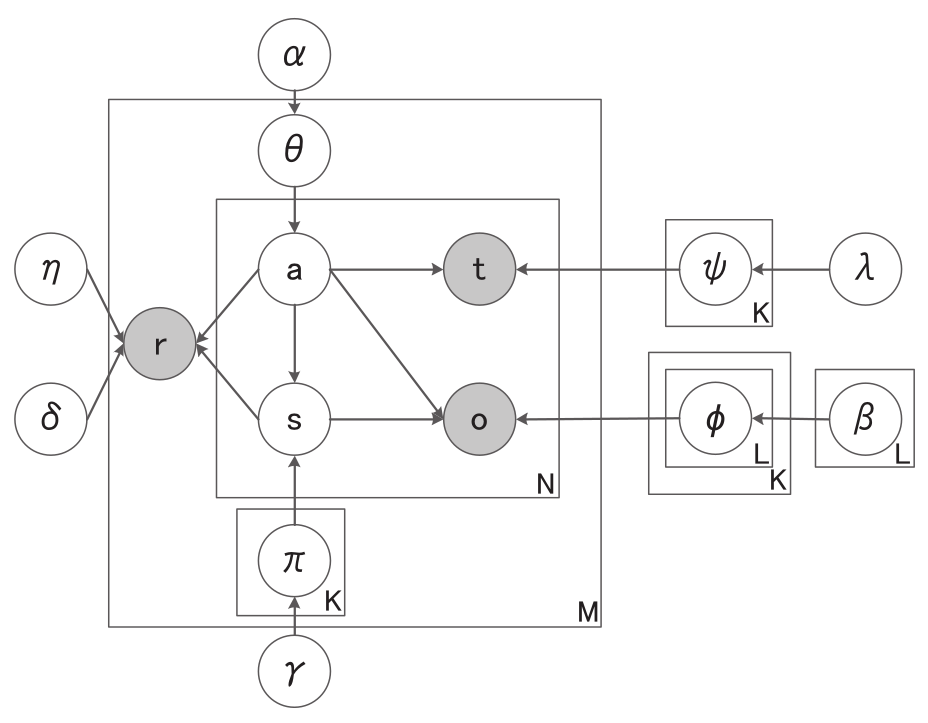
\includegraphics[scale=0.25]{chap3-img/SJASM}
		\caption{مدل نظارت‌شده‌ی مشترک موضوع و احساس \cite{7855825}}
		\label{chap3-fig13}
	\end{figure}


	
\section{مدل‌های چند حالته}
	مدل‌های چندحالته 
	\LTRfootnote{Multimodal}
	دسته‌ای از مدل‌های موضوعی هستند که داده‌ی ورودی در آن‌ها ترکیبی‌ از چند حالت مختلف داده است. در تمام مدل‌های معرفی‌ شده تا این قسمت از پژوهش، داده‌ی ورودی تنها اسناد متنی بودند یا به عبارت دیگر تنها یک حالت از داده به عنوان ورودی به مدل وارد می‌‌شود، اما مدل‌های چندحالته مانند آنچه که در بخش
	\ref{chap3sec5sub1}
	معرفی‌ می‌‌شود بر روی ترکیب همزمان دو یا چند حالت مختلف از داده مثلا تصویر و متن همراه با آن عمل می‌‌کنند.

	
	
	\subsection{مدل نظارت‌شده‌ی شبکه‌‌ی عصبی خود رگرسیو تخمین‌زننده‌ی توزیع سندی}
	\label{chap3sec5sub1}
	مدل نظارت‌شده‌ی شبکه‌‌ی عصبی خود رگرسیو تخمین‌زننده‌ی توزیع سندی\LTRfootnote{Supervised Document Neural Autoregressive Distribution Estimator}
	(SupDocNADE)
	 که در شکل 
	\ref{chap3-fig10}
	مشاهده می‌شود، در سال ۲۰۱۴ توسط
	Zheng
	و همکاران
	\cite{zheng2014topic}
	معرفی‌ شد. این مدل گسترش یافته‌ی مدل
	DocNADE
	می‌ باشد که در بخش
	\ref{chap3sec3sub6}
	معرفی‌ شد
	\cite{zheng2014topic}.
	 در مدل
	SupDocNADE
	داده‌های ورودی تنها اسناد متنی نیستند. ورودی در این مدل تصاویر به همراه توضیح کوتاهی‌ در مورد هر تصویر است که مدل ترکیب این دو 
	نوع داده در کنار یکدیگر را یاد می‌‌گیرد. در این مدل ابتدا هر تصویر با استفاده الگوریتم‌های موجود در حوزه‌ی پردازش تصویر تغییر یافته و به یک سند متنی تبدیل شده و به توضیح مربوط به آن متصل می‌شود و به عنوان بردار ورودی به مدل وارد می‌‌شود
	\cite{zheng2014topic}.
	 تفاوت دیگر این مدل با مدل
	DocNADE
	اضافه کردن یک ساختار بر بایه‌ی شبکه‌ی عصبی در کنار قسمت‌های موجود است که با استفاده از ویژگی‌‌های یاد گرفته شده از ترکیب هر تصویر و متن مربوط به آن عمل طبقه‌بندی را انجام می‌‌دهد
\cite{zheng2014topic}.
	
	\begin{figure}[!b]
		\centering
		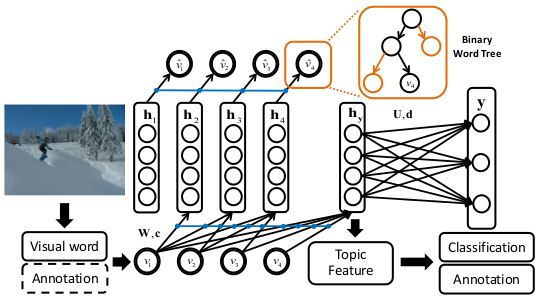
\includegraphics[scale=0.6]{chap3-img/SupDocNADE}
		\caption{مدل نظارت‌شده‌ی شبکه‌‌ی عصبی خود رگرسیو تخمین‌زننده‌ی توزیع سندی \cite{zheng2014topic}}
		\label{chap3-fig10}
	\end{figure}

\section{نتیجه‌گیری}
در این بخش پژوهش‌های پیشین در زمینه‌ی تخمین توزیع، مدل‌سازی موضوع، مدل‌سازی احساس‌-موضوع به صورت مشترک و همچنین مدل‌سازی داده‌های چندوحهی مورد بررسی‌ قرار گرفت. ساختار‌های بررسی‌ شده در این بخش در دو دسته‌ی مدل‌های شبکه‌های عصبی و مدل‌های گرافی‌ بیزین قرار می‌‌گیرند. در این پژوهش با ایده‌
گرفتن از ساختار‌های گرافی بیزین و استفاده از مدل‌های شبکه‌های عصبی هدف ساخت مدلی‌ برای شبیه‌سازی مشترک احساس و موضوع در داده‌های متنی است. در بخش بعدی کلیات نظری مدل پیشنهادی در این پایان‌‌نامه و روابط و ساختار آن به صورت دقیق معرفی‌ و بررسی‌ می‌‌شوند.
 
 	%chap 4
\chapter{مدل پیشنهادی}
\thispagestyle{empty}
\section{مقدمه}
در این بخش روش پیشنهادی در این پژوهش که یک مدل بر پایه‌ی شبکه‌های عصبی برای تشخیص همزمان احساس و موضوع از داده‌های متنی می‌‌باشد ارائه می‌‌گردد. همانطور که پیش از این نیز ذکر شد مدل پیشنهادی در این پژوهش گسترش یافته و تلفیقی از چند مدل شناخته شده در زمینه‌ی مدل‌سازی احساس و موضوع و همچنین تشخیص توزیع‌های احتمالی‌ موجود در داده‌های ورودی می‌‌باشد، لذا در بخش‌های پیش‌ر‌‌و ضمن معرفی‌ کامل این مدل‌ها و تعریف ساختار و 
نحو‌ه‌ی عملکرد هرکدام به مدل پیشنهادی در این پایان‌‌نامه می‌‌رسیم و آن را به طور کامل مورد بررسی‌ قرار داده و تعریف می‌‌کنیم.

\section{مدل پایه}
\label{chap4sec2}
مدل پایه در این پژوهش  شبکه عصبی ماشین بلتزمن محدود می‌باشد که پیش از این در بخش
\ref{chap3sec2sub1}
 آن را
RBM
نامیدیم و به صورت مختصر معرفی‌ گردید.
RBM
که در شکل
\ref{chap4-fig1}
نشان داده شده است،
 RBM 
 یک مدل بدون نظارت برای داده‌های باینری می‌باشد که در دسته‌ی مدل‌های مولد احتمالاتی  قرار می‌گیرد. در این مدل با بیشینه کردن یک تابع انرژی، یا کمینه کردن مقدار منفی‌ آن که به صورت رابطه
\ref{chap4-eq1}
تعریف می‌‌شود، توزیع‌های احتمالی‌ موجود در داده‌های ورودی یاد گرفته می‌شود و از داده‌های ورودی ویژگی‌ استخراج می‌‌گردد. در رابطه‌ی
\ref{chap4-eq1}
مجموعه‌ی پارامترهای مدل به صورت
$\theta = \{W, \textbf{a}, \textbf{b}\}$
است.
$W_{D \times H}$
ماتریس وزن بین لایه‌ی ورودی و لایه‌ی پنهان است، که در آن
$D$
اندازه بردار ورودی و
$H$
اندازه لایه‌ی پنهان هستند.
$\textbf{a}$
بردار بایاس لایه‌ی ورودی با اندازه
$D$
و
$\textbf{b}$
بردار بایاس لایه‌ی پنهان با اندازه
$H$
 است. همان‌طور که در بخش 
 \ref{chap3sec2sub1}
نیز بیان گردید در مدل
 RBM
 داده‌های ورودی و لایه‌ی پنهان متناظر با آن که توسط مدل از بردار ورودی بدست می‌‌آید هر دو در حالت باینری (۰ یا ۱) هستند که این امر یکی‌ از محدودیت‌های این روش است.
\begin{align}
	\centering
	\label{chap4-eq1}
	E(\textbf{v},\textbf{h}) = -\sum_{i} \sum_{j} v_iW_{ij}h_j - \sum_i v_ia_i - \sum_j h_jb_j
\end{align}

در مدل
RBM
احتمال هر ترکیب
$(\textbf{v},\textbf{h})$
از رابطه‌ی
\ref{chap4-eq2}
بدست می‌‌آید که در آن
$Z(\theta)$
تابع قسمت‌بندی است که مقدار آن با استفاده از رابطه‌ی 
\ref{chap4-eq3}
محاسبه می‌شود و تضمین می‌کند که مقدار بدست آمده برای هر ترکیب
$(\textbf{v},\textbf{h})$
یک مقدار صحیح احتمالی‌ (بین ۰ و ۱) می‌‌باشد. در این مدل احتمال هر بردار ورودی از رابطه‌ی
\ref{chap4-eq4}
بدست می‌‌آید.
\begin{align}
	\centering
	\label{chap4-eq2}
	p(\textbf{v},\textbf{h}) = \dfrac{1}{Z(\theta)} e^{-E(\textbf{v},\textbf{h})}
\end{align}
\begin{align}
	\centering
	\label{chap4-eq3}
	Z = \sum_{\textbf{v}, \textbf{h}}e^{-E(\textbf{v},\textbf{h})}
\end{align}
\begin{align}
	\centering
	\label{chap4-eq4}
	p(\textbf{v}) = \sum_{h} \dfrac{1}{Z(\theta)} e^{-E(\textbf{v},\textbf{h})}
\end{align}

برای آموزش این مدل از الگوریتم
CD
که در بخش
\ref{chap2sec7}
معرفی‌ گردید استفاده می‌‌شود. در مراحل آموزش و همچنین آزمودن این مدل نیاز به محاسبه‌ی مقادیر لایه‌ی پنهان مشروط به بردار ورودی و برعکس می‌‌باشد. برای محاسبه
$p(\textbf{h}|\textbf{v})$
داریم:
\begin{align}
	\centering
	\label{chap4-eq5}
	p(\textbf{h}|\textbf{v})=\dfrac{p(\textbf{h},\textbf{v})}{p(\textbf{v})} &=\dfrac{\dfrac{1}{Z}e^{-E(\textbf{v},\textbf{h})}}{\sum_{h}p(\textbf{v},h)}\\\nonumber
								&=\dfrac{\dfrac{1}{Z}e^{vWh^{T}+a^{T}\textbf{v}+b^{T}h}}{\sum_{h}\dfrac{1}{Z}e^{\textbf{v}Wh^{T}+a^{T}\textbf{v}+b^{T}h}}\\\nonumber
								&=\dfrac{e^{\textbf{v}Wh^{T}}.e^{a^{T}\textbf{v}}.e^{b^{T}h}}{\sum_{h}e^{vWh^{T}}.e^{a^{T}\textbf{v}}.e^{b^{T}h}}
								=\dfrac{e^{\textbf{v}Wh^{T}+b^{T}h}}{\sum_{h}e^{\textbf{v}Wh^{T}+b^{T}h}}
								=\dfrac{e^{\textbf{v}Wh^{T}+b^{T}h}}{Z'}\\\nonumber
								&=\dfrac{1}{Z'}exp\left\lbrace \textbf{v}Wh^{T}+b^{T}h\right\rbrace
								=\dfrac{1}{Z'}exp \left\lbrace \sum_{j=1}^{H}\textbf{v}W_jh_j + \sum_{j=1}^{H}b_jh_j \right\rbrace\\\nonumber
								&\Rightarrow p(\textbf{h}|\textbf{v})=\dfrac{1}{Z'}\prod_{j=1}^{H}exp\left\lbrace \textbf{v}W_jh_j + b_jh_j \right\rbrace
\end{align}

\begin{figure}[!t]
	\centering
	\includegraphics[scale=0.5]{chap4-img/RBM}
	\caption{ماشین بلتزمن محدود}
	\label{chap4-fig1}
\end{figure}

در ترم نهایی در رابطه
\ref{chap4-eq5}
مشاهده می‌شود که مقدار
$p(\textbf{h}|\textbf{v})$
برابر است با حاصلضرب
$exp$
به ازای تمام ابعاد بردار
$h$,
لذا نتیجه گرفته می‌‌شود که ابعاد بردار
$h$ 
یعنی‌ همان
$h_j$ها
نسبت به یکدیگر دارای استقلال شرطی هستند. در نتیجه می‌توان رابطه‌ی
\ref{chap4-eq5}
را به شکل رابطه‌ی
\ref{chap4-eq6}
بازنویسی کرد.
\begin{align}
	\centering
	\label{chap4-eq6}
	p(\textbf{h}|\textbf{v})=\prod_{j=1}^{H}p(h_j|\textbf{v})	
\end{align}
\begin{align}
	\centering
	\label{chap4-eq7}
	p(h_j = 1|\textbf{v})=\dfrac{p(h_j=1,\textbf{v})}{p(h_j=1,\textbf{v})+ p(h_j=0,\textbf{v})}
						 &=\dfrac{exp\{\textbf{v}W_j + b_j\}}{exp\{0\} + exp\{\textbf{v}W_j + b_j\}}\\\nonumber
						 &=sigmoid(\textbf{v}W_j + b_j)
\end{align}
\begin{align}
	\centering
	\label{chap4-eq8}
	p(\textbf{h}|\textbf{v})=\prod_{j=1}^{H}sigmoid(\textbf{v}W_j + b_j)
\end{align}
به همین شکل می‌‌توان نتیجه گرفت:
\begin{align}
	\centering
	\label{chap4-eq9}
	p(\textbf{v}|\textbf{h})=\prod_{i=1}^{D}sigmoid(W_i\textbf{h} + a_i)
\end{align}

برای آموزش این مدل فرض می‌‌شود یک مجموعه داده‌ی باینری به صورت
$\{\textbf{v}^{t}\}_{t=1}^{n}$
به عنوان داده‌های آموزش در اختیار است. هدف پیدا کردن پارامتر‌های
$W, \textbf{a}, \textbf{b}$
به صورتی‌ می‌‌باشد که لگاریتم درست‌نمایی برای مشاهده‌ی داده‌های آموزش بیشینه باشد. به بیان ریاضی‌ می‌‌خواهیم مقدار رابطه‌ی
\ref{chap4-eq10}
را نسبت به مجموعه پارامتر‌های
$\theta = \{W, \textbf{a}, \textbf{b}\}$
بیشینه کنیم.
\begin{align}
	\centering
	\label{chap4-eq10}
	\ell(W, \textbf{a}, \textbf{b}) &= \sum_{t=1}^{n}\log p(\textbf{v}^t) = \sum_{t=1}^{n}\log \sum_h p(\textbf{v}^t, h)\\\nonumber
									&= \sum_{t=1}^{n}\log\dfrac{1}{Z} \sum_h e^{-E(\textbf{v}^t,h)} = \sum_{t=1}^{n}\log \sum_h e^{-E(\textbf{v}^t,h)} - n\log Z\\\nonumber
									&= \sum_{t=1}^{n}\log\sum_h e^{-E(\textbf{v}^t,h)} - n\log\sum_{\textbf{v},\textbf{h}}exp\left\lbrace -E(\textbf{v}^t,h)\right\rbrace\\\nonumber
\end{align}
رابطه‌ی
\ref{chap4-eq10}
را معاد‌له لگاریتم درست‌نمایی تعریف می‌‌کنیم که برای بیشینه کردن آن نسبت به مجموعه پارامتر‌های
$\theta$
باید از آن نسبت به پارامترهای این مجموعه مشتق گرفت.
\begin{align}
	\centering
	\label{chap4-eq11}
	\triangledown_\theta \ell(\theta) &= \triangledown_\theta \sum_{t=1}^{n} \log \sum_h exp \left\lbrace -E(\textbf{v}^t, \textbf{h}) \right\rbrace - n\triangledown_\theta \log \sum_{\textbf{v}, \textbf{h}} exp \left\lbrace -E(\textbf{v}, \textbf{h}) \right\rbrace \\\nonumber
	&=\sum_{t=1}^{n} \dfrac{\sum_h exp \left\lbrace -E(\textbf{v}^t, \textbf{h}) \right\rbrace \triangledown_\theta -E(\textbf{v}^t, \textbf{h})}{\sum_h exp \left\lbrace -E(\textbf{v}^t, \textbf{h}) \right\rbrace} - n \dfrac{\sum_{v,h} exp \left\lbrace -E(\textbf{v}, \textbf{h}) \right\rbrace \triangledown_\theta -E(\textbf{v}, \textbf{h})}{\sum_{v,h} exp \left\lbrace -E(\textbf{v}, \textbf{h}) \right\rbrace}\\\nonumber
	&=\sum_{t=1}^{n}E_{p(\textbf{h}|\textbf{v}^t)}[\triangledown_\theta -E(\textbf{v}^t, \textbf{h})] - nE_{p(\textbf{v},\textbf{h})}[\triangledown_\theta -E(\textbf{v}, \textbf{h})]
\end{align}
\begin{align}
	\centering
	\label{chap4-eq12}
	\triangledown_{W} -E(\textbf{v},\textbf{h}) = \textbf{v}^T\textbf{h} \qquad  \triangledown_{\textbf{a}} -E(\textbf{v},\textbf{h}) = \textbf{v} \qquad  \triangledown_{\textbf{b}} -E(\textbf{v},\textbf{h}) = \textbf{h}
\end{align}

ترم اول سمت راست رابطه
\ref{chap4-eq11}
یک مقدار مورد انتظار برای مشتق تابع انرژی نسبت به توزیع شرطی دادهای آموزش،
$p(\textbf{h}|\textbf{v})$،
و ترم دوم آن یک مقدار مورد انتظار برای تابع انرژی نسبت به توزیع مشترک برای تمام حالت های  مدل
$p(\textbf{v},\textbf{h})$
 است. با توجه به رابطه‌ی
\ref{chap4-eq12}
برای بدست آوردن ترم اول در رابطه‌ی
\ref{chap4-eq13}
برای هر بردار
$\textbf{v}$
مقدار
$\textbf{h}$
متناظر با آن را با استفاده از رابطه‌ی
\ref{chap4-eq8}
بدست می‌‌آوریم. از آن‌جا که ترم دوم رابطه‌ی
\ref{chap4-eq11}
به توزیع تمام حالات موجود برای مدل
($p(\textbf{v},\textbf{h})$)
وابسته است محاسبه‌ی آن برای ما امکان‌پذیر نیست و باید مقدار آن را به صورت تقریبی بدست آوریم. الگوریتم
CD
در اینجا وارد عمل می‌شود و مقدار مورد انتظار از مشتق تابع انرژی بر روی یک توزیع مشترک را با یک تخمین نقطه‌ای جایگزین می‌‌کند. به این صورت که یک بردار از داده‌های آموزش انتخاب کرده و با استفاده از الگوریتم نمونه‌برداری
Gibbs
و همچنین روابط
\ref{chap4-eq9}
و
\ref{chap4-eq8}
مقادیر بردار‌های
$\textbf{h}$
و
$\textbf{v}$
را به ترتیب محاسبه می‌کند. یک چرخه‌‌ی کامل الگوریتم نمونه‌برداری
Gibbs
شامل محاسبه‌ی بردار
$\textbf{h}$
از یک بردار
$\textbf{v}$
و سپس ساختن مجدد بردار
$\textbf{v}$
از این بردار
$\textbf{h}$
می‌باشد. این چرخه تا زمانی که به یک حالت تعادل دست یابید ادامه پیدا می‌کند، در حالت تعادل مقدار بردارهای
$\textbf{v}$
و
$\textbf{h}$
بدست آماده برابر با مقدار مورد انتظار برای ترم دوم رابطه
\ref{chap4-eq13}
در نظر گرفته می‌‌شود. همچنین با استفاده از مقادیر بدست آمده برای بردارهای
$\textbf{v}$
و
$\textbf{h}$
مقدار روابط
\ref{chap4-eq14}
و
\ref{chap4-eq15}
نیز محاسبه می‌‌گردد.
\begin{align}
	\centering
	\label{chap4-eq13}
	\triangledown_W \ell(W, \textbf{a}, \textbf{b})=\sum_{t=1}^{n} \textbf{v}^{t^T} \hat{h}^t - nE_{p(\textbf{v},\textbf{h})}[\textbf{v}^T\textbf{h}]
\end{align}
\begin{align}
	\centering
	\label{chap4-eq14}
	\triangledown_{\textbf{a}} \ell(W, \textbf{a}, \textbf{b})=\sum_{t=1}^{n} \textbf{v}^{t} - nE_{p(\textbf{v},\textbf{h})}[\textbf{v}] 
\end{align}
\begin{align}
	\centering
	\label{chap4-eq15}
	\triangledown_{\textbf{b}} \ell(W, \textbf{a}, \textbf{b})=\sum_{t=1}^{n} \textbf{h}^{t} - nE_{p(\textbf{v},\textbf{h})}[\textbf{h}] 
\end{align}

همان‌طور که پیش از این در بخش
\ref{chap2sec7}
بیان شد، آقای
Hinton
نشان داد که تنها تعداد کمی‌ چرخه‌‌‌ی نمونه‌برداری
Gibbs
برای بدست آوردن تقریبی مناسب نسبت به توزیع
$p(\textbf{v},\textbf{h})$
کافی‌ می‌‌باشد
\cite{hinton2002training}\cite{carreira2005contrastive}.
اگرچه پیاده‌سازی‌های انجام شده نشان داده است که تنها انجام یک چرخه‌ی
Gibbs
برای محاسبه‌ی یک تقریب صحیح از جهت حرکت گرادیان کافی‌ می‌‌باشد
\cite{carreira2005contrastive}.
در نهایت برای کمینه کردن تابع انرژی رابطه‌ی بروز‌رسانی کردن مجموعه پارامتر‌های 
$\theta$
 به شکل رابطه‌ی
\ref{chap4-eq16}
می‌گردد که در آن
$\epsilon$
ضریب یادگیری می‌‌باشد و به صورت تجربی‌ مشخص گردد.
\begin{align}
	\centering
	\label{chap4-eq16}
	\theta_{t+1} = \theta_t + \epsilon \left( E_{P_{data}}[\triangledown_{\theta} -E(\textbf{v},\textbf{h})] - E_{P_{model}}[\triangledown_{\theta} -E(\textbf{v},\textbf{h})] \right) 
\end{align}

\section{ماشین بلتزمن محدود با واحدهای قابل مشاهده صحیح}
\label{chap4sec3}
ساختار معرفی‌ شده در بخش
\ref{chap4sec2}
مدل استاندارد
RBM
می‌باشد که به صورت دقیق مورد بررسی‌ قرار گرفت و به عنوان مدل پایه برای روش پیشنهادی در این پژوهش در نظر گرفته می‌‌شود. برای تعریف ساختار مورد نظر در این پایان‌‌نامه جهت مدل‌سازی احساس و موضوع نیاز به معرفی‌ و بررسی‌ نمونه‌های پیچیده‌تری از مدل
RBM
استاندارد می‌‌باشد.

محدود بودن به حالت باینری برای داده‌های ورودی و همچنین طول ثابت برای آن‌ها دو اشکال اساسی در مدل
RBM
استاندارد می‌‌باشند. حال فرض کنید ساختاری داریم که در آن داده‌های ورودی همچنان دارای طول ثابت هستند اما به جای حالت باینری می‌‌توانند هر مقدار صحیح غیر منفی‌ از یک حداقل تا یک حداکثر را اختیار کنند. در این ساختار که در شکل
\ref{chap4-fig2}
نشان داده شده است به جای بردار ورودی ما ماتریس ورودی خواهیم داشت، و هر داده به صورت یک ماتریس با درایه‌های ۰ و ۱ به مدل وارد می‌‌شود. در مدل
RBM
استاندارد ورودی تنها یک بردار با طول ثابت با درایه‌های ۰ و یا ۱ بود، که حضور و یا عدم حضور هر یک از ویژگی‌‌های متناظر با درایه‌ی مورد نظر در بردار ورودی را مشخص می‌‌کند. اما در این مدل هر داده‌ی ورودی به صورت ماتریسی متشکل از ۰ یا ۱ می‌‌باشد.

فرض کنید در مساله‌ای‌ که با آن سرو کار داریم هر داده‌ی ورودی دارای
D
ویژگی‌ می‌‌باشد که هر یک از این ویژگی‌ها می‌‌توانند 
K
مقدار داشته باشند. مدل
RBM
استاندارد توانایی کار کردن با یک چنین داده‌های ورودی را ندارد چرا که در آن داده‌های ورودی تنها می‌‌توانند یک بردار با طول ثابت و شامل ۰ و ۱ باشند. در این مدل جدید هر داده‌ی ورودی به صورت ماتریسی با اندازه
$K \times D$
در نظر گرفته می‌شود که همان‌طور که بیان شد
D
طول بردار ورودی یا همان تعداد ویژگی‌های مساله و
K
بیشینه مقداری می‌‌باشد که هر ویژگی‌ می‌‌تواند داشته باشد. برای ساخت این ماتریس ابتدا تمام درایه‌های آن را صفر می‌‌کنیم و سپس برای هر ستون یا به عبارتی برای هر ویژگی‌ سطر متناظر با مقدار آن ویژگی‌ را ۱ می‌‌کنیم. در این حالت به ازای هر داده‌ی ورودی یک ماتریس شامل ۰ و ۱ داریم با این خصوصیت که در هر ستون آن تنها مقدار یک سطر  ۱ می‌‌باشد و مابقی سطرها مقدارشان ۰ می‌‌باشد.
\begin{figure}[!t]
	\centering
	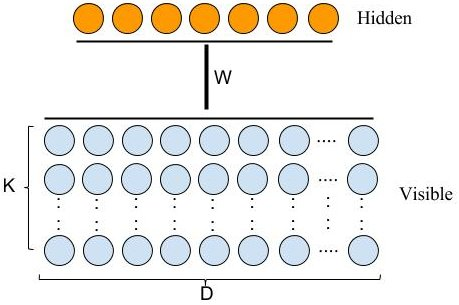
\includegraphics[scale=0.5]{chap4-img/MRBM}
	\caption{ماشین بلتزمن محدود با واحدهای قابل مشاهده صحیح}
	\label{chap4-fig2}
\end{figure}

تا به اینجا تفاوت این ساختار با مدل
RBM
استاندارد را معرفی‌ کردیم. از نظر تفاوت در فضای پارامتری، در مدل
RBM
استاندارد ماتریس وزن بین لایه‌ی قابل مشاهده و لایه‌ی پنهان یک ماتریس دو بعدی بود، اما در این ساختار به دلیل تغییر در شکل ورودی ماتریس وزن بین این دو لایه یک ماتریس سه بعدی می‌‌باشد. در این ساختار نیز مانند مدل
RBM
استاندارد که در آن تمام ابعاد بردار ورودی به تمام واحد‌های لایه‌ی پنهان متصل بودند، در اینجا نیز یک اتصال کامل بین تمام قسمت‌های ماتریس ورودی و تمام واحد‌های لایه‌ی پنهان بر قرار می‌‌باشد. تفاوت دیگر این دو ساختار در فضای پارامتر‌ها مربوط به بایاس لایه‌ی قابل مشاهده می‌‌باشد. برخلاف مدل
RBM
استاندارد که برای لایه‌ی قابل مشاهده یک بردار بایاس وجود داشت در ساختار نشان داده شده در شکل
\ref{chap4-fig2}
ما یک ماتریس دو بعدی برای بایاس خواهیم داشت که در فرآیند آموزش درایه‌های آن یاد گرفته می‌‌شوند.

با توجه به تغییرات بیان شده در ساختار
RBM
استاندارد و همچنین تغییرات اعمال شده در فضای پارامتر‌های مساله، روابط
\ref{chap4-eq1}
تا
\ref{chap4-eq9}
نیز دچار تغییرات اساسی‌ می‌‌گردند که در اینجا به بیان آن‌ها می‌پردازیم. فرض کنید قصد مدل‌سازی بردا‌های ورودی
$\textbf{v}$
با مدلی‌ مانند آنچه در شکل
\ref{chap4-fig2}
نشان داده شده است را داریم. اگر هر داده‌ی
$\textbf{v}$
به شکل
$\textbf{v} \in \{1, ..., K\}^D$
باشد، که در آن همان‌طور که پیش از این بیان کردیم،
$K$
بیشینه مقداری می‌‌باشد که هر ویژگی‌ می‌‌تواند دریافت کند و
$D$
اندازه داده‌های ورودی است. همچنین بردار پنهان به شکل
$\textbf{h} \in \{0,1\}^H$
می‌ باشد. اگر
$\textbf{V}$
ماتریس باینری قابل مشاهده باشد که برای هر داده‌ی ورودی ساخته می‌‌شود، در این صورت تابع انرژی برای حالت
$\{\textbf{V},\textbf{h}\}$
به شکل رابطه
\ref{chap4-eq17}
تعریف می‌‌شود.
\begin{align}
	\centering
	\label{chap4-eq17}
	E(\textbf{V},\textbf{h})=-\sum_{i=1}^{D}\sum_{j=1}^{H}\sum_{k=1}^{K}W_{ijk}h_jv_{ik}-\sum_{i=1}^{D}\sum_{k=1}^{K}v_{ik}a_{ik} - \sum_{j=1}^{H}h_jb_j
\end{align}

در رابطه‌ی‌
\ref{chap4-eq17}
نیز مانند حالت قبل
$\{W, a, \textbf{b}\}$
مجموعه پارامتر‌های مدل می‌‌باشند که در آن
$W_{D \times H \times K}$
ماتریس سه‌ بعدی وزن بین واحد قابل مشاهده‌ی
$i$ام
 و مقدار
$k$ام
 و واحد
$j$ام 
بردار لایه‌ی پنهان می‌‌باشد، همچنین در رابطه‌ی
\ref{chap4-eq17}، $a_{D \times K}$
ماتریس دو بعدی بایاس برای لایه‌ی قابل مشاهده و
$\textbf{b}_{1 \times H}$
بردار بایاس برای لایه‌ی پنهان می‌‌باشد. احتمالی‌ که این ساختار به ماتریس باینری قابل مشاهده‌ی
$\textbf{V}$
اختصاص می‌‌دهد از رابطه‌ی
\ref{chap4-eq18}
 بدست می‌‌آید.
 \begin{align}
 	\centering
 	\label{chap4-eq18}
 	p(\textbf{V}) = \sum_{h} \dfrac{1}{Z} e^{-E(\textbf{V},\textbf{h})} \quad\quad ; \quad
 	Z = \sum_{\textbf{V},\textbf{h}} e^{-E(\textbf{V},\textbf{h})} 
 \end{align}

در این ساختار توزیع‌های شرطی برای لایه‌های قابل مشاهده و پنهان به شکل روابط
\ref{chap4-eq19}
و
\ref{chap4-eq20}
هستند. همان‌طور که مشاهده می‌‌گردد توزیع شرطی مربوط به لایه‌ی قابل مشاهده کاملا با رابطه‌ی
\ref{chap4-eq9}
که برای مدل
RBM
استاندارد تعریف گردید تفاوت دارد، و توزیع مورد استفاده در رابطه‌ی
\ref{chap4-eq19}
 مانند آنچه که در بخش
\ref{chap2sec9}
توضیح داده شد از تابع
Softmax
استفاده می‌‌کند. دلیل استفاده از تابع
Softmax
به جای تابع سیگموید که در مدل
RBM
استاندارد از آن استفاده می‌‌شد تغییر در ساختار ورودی و لایه‌ی قابل مشاهده می‌‌باشد. با توجه به اینکه هر ویژگی‌ تنها یک مقدار از
$K$
مقدار ممکن را می‌‌تواند داشته باشد، یا به عبارتی در هر ستون ماتریس باینری
$\textbf{V}$
 در لایه‌ی قابل مشاهده تنها یک ۱ می‌‌تواند وجود داشته باشد، لذا برای هر ستون در این ماتریس از یک تابع
Softmax
استفاده می‌گردد و احتمال یک بودن هر یک از این
$K$
 مقدار حساب می‌گردد و سپس با تولید یک عدد تصادفی با توجه به احتمالات بدست آمده برای هر یک از
$K$
مقدار ممکن برای هر ویژگی‌، مقدار آن ویژگی‌ تعیین می‌‌گردد. در حقیقت فرمول
\ref{chap4-eq19}
برای توزیع احتمالی‌ لایه قابل مشاهده این اطمینان را به ما می‌دهد که مقادیر بدست آماده برای هر ویژگی‌ به ازای
$K$
مقدار ممکن برای آن، یک توزیع چند احتمالی‌ چندجمله‌ای ازدرجه‌ی
$K$
می‌باشد.
\begin{align}
	\centering
	\label{chap4-eq19}
	p(v_{ik}=1|\textbf{h})=\dfrac{exp(a_{ik}+\sum_{j=1}^{H}h_jW_{ijk})}{\sum_{k=1}^{K}exp(a_{ik}+\sum_{j=1}^{H}h_jW_{ijk})}
\end{align}
\begin{align}
	\centering
	\label{chap4-eq20}
	p(h_{j}=1|\textbf{V})=\sigma \left( b_j +  \sum_{i=1}^{D}\sum_{k=1}^{K}W_{ijk}v_{ik} \right)
\end{align}

\section{مدل مولد براساس تعداد کلمات}
\label{chap4sec4}

مدلی‌ که در این بخش به صورت کامل آن را شرح می‌‌دهیم و گسترش یافته‌ی مدل معرفی‌ شده در بخش
\ref{chap4sec3}
می‌باشد در واقع همان مدل
RS
 است که در بخش
\ref{chap3sec3sub5}
به صورت مختصر آن را معرفی‌ کردیم. بررسی‌ مدل
RS
در درک مدل پیشنهادی حائز اهمیت می‌‌باشد، چرا که مدل پیشنهادی در این پایان‌‌نامه بر روی ساختار این مدل سوار شده و گسترش یافته‌ی آن می‌‌باشد. مدل
RS
 همان‌طور که در بخش
\ref{chap3sec3sub5}
بیان شد یک مدل مولد احتمالی‌ بر اساس تعداد کلمات می‌‌باشد که به صورت بدون نظارت به مدل‌سازی موضوع در داده‌های متنی می‌‌پردازد.

در بحث مدل‌سازی موضوع پیش از آموزش مدل ابتدا یک بار تمام مجموعه سند پیمایش می‌‌شود و تمام کلمات متمایز در تمام اسناد مشخص شده و همراه با ایندکس هرکدام ذخیره می‌‌شوند. به عبارت دیگر قبل از شروع مرحله‌ی آموزش ابتدا یک لغت‌نامه از تمام کلمات متمایز در مجموعه اسناد ساخته می‌‌شود. پس از پایان این مرحله و ساخت لغت‌نامه به مدل بخش
\ref{chap4sec3}
بر می‌‌گردیم و مدل معرفی‌ شده در آن جا را در این حالت اندکی‌ بررسی‌ می‌‌کنیم. در بخش
\ref{chap4sec3}
گفته شد که مقدار هر ویژگی‌ می‌‌تواند از یک مینیمم تا یک بیشینه باشد، حال فرض کنید که بحث مدل‌سازی موضوع بر روی داده‌های متنی می‌‌باشد و پس از ساخت لغت‌نامه می‌خواهیم از مدل بخش
\ref{chap4sec3}
استفاده کنیم. در اینجا مقدار هر ویژگی‌ برابر با اندیس یکی‌ از کلمات لغت‌نامه می‌‌باشد. هر سند ورودی پس از انجام پیش پردازش‌های لازم به صورت یک دنباله از کلمات تبدیل شده است که هر کدام از این کلمات برابر با یکی‌ از کلمات لغت‌نامه می‌‌باشند. به این ترتیب در ماتریس ورودی به مدل که یک ماتریس به انداز‌ه‌ی
$K \times D$
می‌ باشد
$K$
برابر با اندازه لغت‌نامه می‌‌باشد و
$D$
نشان دهنده‌ی طول سند متنی می‌‌باشد. در این حالت برای هر ستون مقدار سطر متناظر با اندیس آن کلمه در لغت‌نامه برابر با ۱ می‌‌شود و دیگر درایه‌های آن ستون همچنان صفر باقی‌ می‌‌مانند.

حال فرض کنید که برای مدل کردن داده‌های متنی با استفاده از ساختار معرفی‌ شده در بخش
\ref{chap4sec3}
برای هر سند یک شبکه‌ی
RBM
جدا می‌‌سازیم که به تعداد کلمات همان سند دارای واحد
Softmax
می‌باشد. در این حالت ورودی دیگر یک ماتریس باینری نخواهد بود و به صورت برداری از تعداد کلمات موجود در آن سند می‌‌باشد که می‌‌توانیم ترتیب را در آن‌ها نادیده بگیریم. رابطه‌ی محاسبه‌ی انرژی در این حالت به شکل رابطه‌ی
\ref{chap4-eq21}
می‌‌باشد که در آن
$\hat{v}^k = \sum_{i=1}^{D}v_{ik}$
است. به عبارت دیگر
$\hat{\textbf{v}}$
برداری می‌‌باشد با طول
$K$
که 
$K$
همان اندازه لغت‌نامه می‌‌باشد و از محاسبه‌ی حاصل جمع سطر‌های ماتریس باینری ورودی بدست می‌‌آید.
\begin{align}
	\centering
	\label{chap4-eq21}
	E(\textbf{v},\textbf{h})=-\sum_{j=1}^{H}\sum_{k=1}^{K}W_{jk}h_j\hat{v}_{k}-\sum_{k=1}^{K}v_{k}a_{k} - D\sum_{j=1}^{H}h_jb_j
\end{align}
با تغییرات انجام گرفته در لایه‌ی قابل مشاهده و تعویض ساختار ورودی، در ماتریس وزن بین این لایه و لایه‌ی پنهان و همچنین بایاس لایه‌ی قابل مشاهده تغییراتی‌ رخ می‌‌دهد. در رابطه
\ref{chap4-eq21}، $W$
ماتریسی با اندازه‌ی
$K \times H$
و
$\textbf{a}$
یک بردار با اندازه‌ی
$1 \times K$
می‌ باشند.

در این مدل که آن را
Softmax
تکرار شده نامیدیم روابط شرطی محاسبه‌ی لایه‌ی قابل مشاهده و لایه‌ی پنهان به شکل روابط
\ref{chap4-eq22}
و
\ref{chap4-eq23}
می‌ باشند.
\begin{align}
	\centering
	\label{chap4-eq22}
	p(v_{i}=w|\textbf{h})=\dfrac{exp(a_{w}+\sum_{j=1}^{H}h_jW_{wj})}{\sum_{k=1}^{K}exp(a_{w}+\sum_{j=1}^{H}W_{wj})}
\end{align}
\begin{align}
	\centering
	\label{chap4-eq23}
	p(h_{j}=1|\textbf{V})=\sigma \left( Db_j + \sum_{k=1}^{K}W_{kj}\hat{v}_k \right)
\end{align}
همانطور که مشاهده می‌‌شود در روابط
\ref{chap4-eq21}
و
\ref{chap4-eq23}
ترم بایاس برای لایه‌ی پنهان با اندازه سند جاری نیز متناسب می‌‌باشد. وجود این تناسب در پیاده‌سازی‌های تجربی‌ و هنگامی که با اسناد با طول‌های متفاوت سر و کار داریم بسیار حیاتی می‌‌باشد. در این مدل نیز برای آموزش از الگوریتم
CD
استفاده می‌‌شود، رابطه‌ی بروزرسانی نیز همان است که در بخش
\ref{chap4sec2}
و رابطه
\ref{chap4-eq16}
نشان داده شد با این تفاوت که به جای بردار باینری برای لایه‌ی قابل مشاهده از مقدار آن بر اساس تعداد کلمات استفاده می‌‌شود. برای مثال در یک مجموعه از
N
سند آموزش که به شکل
$\{\textbf{V}_n\}_{n=1}^{N}$
می‌باشد رابطه‌ي بروزرسانی برای یک عنصر ماتریس وزن به شکل رابطه‌ی
\ref{chap4-eq25}
می‌ باشد.
\begin{align}
	\centering
	\label{chap4-eq24}
	\dfrac{1}{N}\sum_{n=1}^{N}\dfrac{\partial\log P(\textbf{V}_n)}{\partial W_{jk}} = E_{P_{data}}[\hat{v}_kh_j]-E_{P_{model}}[\hat{v}_kh_j]
\end{align}
\begin{align}
	\centering
	\label{chap4-eq25}
	\triangle W_{jk} = \alpha \left( E_{P_{data}}[\hat{v}_kh_j]-E_{P_{model}}[\hat{v}_kh_j]  \right)
\end{align}

\section{مدل پیشنهادی مولد احتمالی احساس/موضوع}
\label{chap4sec5}



مدل معرفی‌ شده در این پایان‌‌نامه یک مدل مولد احتمالاتی شبکه عصبی برای مدل‌سازی موضوع و احساس در داده‌های متنی است. این روش گسترش یافته‌ی مدل
RS
است که در بخش
\ref{chap4sec4}
معرفی شد. در مدل پیشنهادی که در شکل
\ref{chap4-fig3}
نشان داده شده است، مشاهده می‌‌گردد که این روش نیز یک ساختار دو لایه دارد که در سمت لایه‌ی قابل مشاهده‌ی آن یک بردار متناظر با برچسب هر سند که در این پژوهش ما آن را به عنوان بردار متناظر با احساس هر سند تعبیر می‌کنیم به ساختار مدل اضافه شده است. بردار ورودی در این ساختار در قسمت
Visible
یک بردار با طولی ثابت و به اندازه‌ی اندازه لغت‌نامه یا همان تعداد کلمات متمایز در متن است که در آن تعداد تکرار کلمات مشخص شده است.

در مدل معرفی‌ شده در بخش
\ref{chap4sec3}
که در شکل
\ref{chap4-fig2}
نشان داده شده است، هر سند ورودی پس از انجام پیش‌پردازش‌های مورد نیاز و تبدیل به یک دنباله از کلمات به صورت یک ماتریس به مدل وارد می‌‌شود. در نظر گرفتن یک چنین ساختاری برای هر سند ورودی به این معنی‌ می‌‌باشد که جایگاه هر کلمه در متن برای ما مهم می‌‌باشد و ترتیب کلمات در هر سند درنظر گرفته می‌‌شود که این امر موجب بزرگ شدن فضای پارامتر‌های مساله (سه‌ بعدی شدن ماتریس وزن و دو بعدی شدن ماتریس بایاس برای لایه‌ی قابل مشاهده) و کند شدن فرآیند آموزش می‌‌گردد. علاوه بر این در بحث مدل‌سازی موضوع حضور و عدم حضور کلمات به همراه فرکانس تکرار آن‌ها دارای اهمیت می‌‌باشد نه محل قرار گرفتن هر کلمه در متن، چرا که تمام مدل‌های بررسی‌ شده در این پژوهش و همچنین مدل پیشنهادی بر اساس کیسه کلمات
(\ref{chap2sec10})
رفتار می‌‌کنند که در آن ترتیب کلمات در نظر گرفته نمی‌‌شود.  در شکل
\ref{chap4-fig4}
یک نمونه از ماتریس ورودی به مدل معرفی‌ شده در بخش
\ref{chap4sec3}
نشان داده شده است. در این مثال سند ورودی به مدل پس از انجام پیش‌پردازش‌های لازم به یک دنباله از پنج کلمه تبدیل شده است، یک کلمه از لغت‌نامه  مانند 
Student
در سند ورودی در دو جایگاه مختلف در سند نشان داده شده است، با توجه به ساختار معرفی‌ شده در بخش
\ref{chap4sec3}
و ماتریس‌های وزن و بایاس سه‌ و دو بعدی، نتیجه گرفته می‌‌شود برای این کلمه دو مقدار متفاوت برای وزن و بایاس آن (یکی برای x
 و یکی برای 
 (y
 تعریف می‌‌شود. لذا متناسب با اینکه کلمه در کجای سند ورودی قرار داشته باشد می‌تواند وزن‌های متفاوتی داشته باشد. این امر موجب بزرگ شدن ماتریس ورودی،  طولانی‌ شدن فرایند آموزش و در نظر گرفتن تفاوت برای محل قرار گرفتن هر کلمه در متن می‌گردد. در مدل پیشنهادی در این پژوهش که در ادامه شرح داده می‌‌شود با تغییر ساختار ورودی از این مشکلات اجتناب می‌‌گردد.

\begin{figure}[!t]
	\centering
	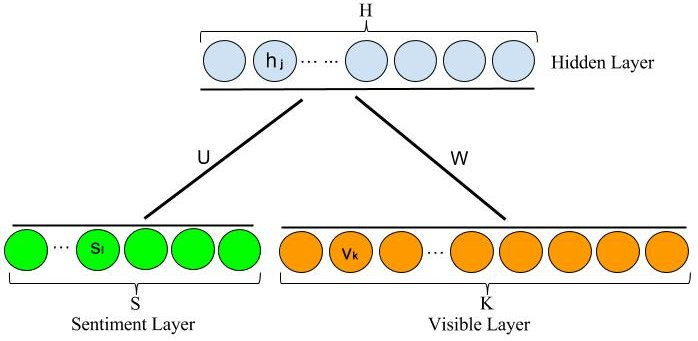
\includegraphics[scale=0.5]{chap4-img/SRS}
	\caption{مدل پیشنهادی مولد احتمالی احساس/موضوع با Softmax تکرار شده}
	\label{chap4-fig3}
\end{figure}

\begin{figure}[!t]
	\centering
	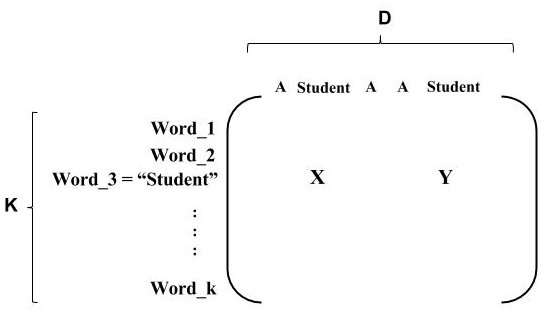
\includegraphics[scale=0.4]{chap4-img/example}
	\caption{یک سند ورودی با ۵ کلمه در مدل بخش \ref{chap4sec3}}
	\label{chap4-fig4}
\end{figure}

در مدل پیشنهادی در این پژوهش و همچنین مدل
RS
هر سند به صورت یک بردار شامل تعداد کلمات به مدل وارد می‌‌شود. در این ساختار مانند آنچه که در شکل
\ref{chap4-fig3}
نشان داده شده است طول بردار ورودی برابر با اندازه لغت‌نامه یا همان تعداد کلمات متمایز در مجموعه سند در نظر گرفته می‌‌شود که درایه‌های آن تعداد تکرار هر کلمه از لغت‌نامه در سند جاری را نشان می‌‌دهند. در این حالت در واقع وزن‌ها برای هر کلمه به اشتراک گذاشته می‌‌شوند فارغ از اینکه این کلمه در کجای سند ورودی قرار دارد. به طور مثال برای کلمه‌ی‌
$n$ام 
لغت‌نامه یک وزن و یک بایاس تعریف می‌‌گردد و این کلمه در هر جای سند ورودی قرار داشته باشد وزنش تغییری نخواهد کرد و در فرآیند آموزش تنها یک وزن و یک بایاس برای هر کلمه یاد گرفته می‌‌شود. با توجه به ساختار مدل که در شکل
\ref{chap4-fig3}
نشان داده شده است، برای هر سند متنی برداری با اندازه لغت‌نامه که شامل تعداد تکرار هر کلمه از لغت‌نامه در آن سند می‌‌باشد و همچنین یک بردار باینری که نشان دهنده احساس سند جاری می‌‌باشد به عنوان ورودی به شبکه وارد می‌‌شوند، و توزیع‌های موجود برروی کلمات مختلف در هر موضوع و همچنین احساس مرتبط با آن‌ها توسط مدل در لایه‌‌ی پنهان استخراج می‌‌شوند.

مدل پیشنهادی در این پژوهش 
(شکل \ref{chap4-fig3})
 یک مدل نظارت شده می‌‌باشد که برای هر سند با مینیمم کردن یک تابع انرژی که به شکل رابطه‌‌ی
\ref{chap4-eq26}
تعریف می‌‌شود، به مدل‌سازی احساس و موضوع به صورت مشترک در داده‌های متنی می‌‌پردازد. با اضافه شدن یک لایه‌ی جدید در این مدل به همراه ماتریس وزن و همچنین بردار بایاس همراه با آن، روابط موجود نسبت به ساختار‌های پیشین تغییر می‌کند. همان‌طور که در رابطه‌ی
\ref{chap4-eq26}
مشاهده می‌‌شود، برای محاسبه‌ی انرژی در مدل پیشنهادی ترم‌های مربوط به وزن و بایاس لایه‌ی احساس نیز در بدست آوردن مقدار نهایی مشارکت دارند. پس از محاسبه‌ی مقدار انرژی به کمک رابطه‌ی
\ref{chap4-eq26}،
 با استفاده از فرمول
\ref{chap4-eq27}
احتمالی‌ که مدل به هر سند و ‌لایه‌ی احساس همراه با آن اختصاص می‌‌دهد، محاسبه می‌‌گردد. برای آموزش این مدل و بروزرسانی پارامترهای شبکه که شامل ماتریس‌های وزن بین لایه‌ی قابل‌مشاهده و پنهان و همچنین لایه‌ی احساس و پنهان می‌‌باشند و همچنین بایاس‌های هر سه‌ لایه از الگوریتم
CD
که در بخش
\ref{chap2sec7}
معرفی‌ شده به شکل رابطه‌ی
\ref{chap4-eq28}
استفاده می‌‌شود.
\begin{align}
	\label{chap4-eq26}
	E(\textbf{V},\textbf{s},\textbf{h})=-\sum_{j=1}^{H}\sum_{k=1}^{K}W_{kj}h_j\hat{v}_{k}&-\sum_{j=1}^{H}\sum_{l=1}^{S}U_{lj}h_js_l\\\nonumber
	&-\sum_{k=1}^{K}v_{k}a_{k} -\sum_{l=1}^{S}s_lc_l- D\sum_{j=1}^{H}h_jb_j
\end{align}
\begin{align}
	\centering
	\label{chap4-eq27}
	p(\textbf{v},\textbf{s},\textbf{h}) = \dfrac{1}{Z} e^{-E(\textbf{v},\textbf{s},\textbf{h})} \Rightarrow
	p(\textbf{v},\textbf{s}) = \dfrac{1}{Z} \sum_{h}  e^{-E(\textbf{v},\textbf{s},\textbf{h})} \ \ ,
	Z = \sum_{\textbf{v}}\sum_{\textbf{s}}\sum_{\textbf{h}} e^{-E(\textbf{v},\textbf{s},\textbf{h})} 
\end{align}
\begin{align}
	\centering
	\label{chap4-eq28}
	\triangle\theta = \alpha \left( E_{P_{data}}[\theta]-E_{P_{model}}[\theta]\right) \Rightarrow \theta_{t+1} = \theta_t + \triangle\theta
\end{align}
در رابطه
\ref{chap4-eq26}، $\theta=\{W, U, \textbf{a}, \textbf{b}, \textbf{c} \}$
مجموعه پارامتر‌های مدل می‌‌باشد که در آن
$W_{K \times H}$
ماتریس وزن بین بردار
$Visible$
و لایه‌ی
$Hidden$، $U_{S \times H}$
ماتریس وزن بین لایه‌ی
$Sentiment$
و لایه‌ی
$Hidden$
و
$\textbf{a}$، $\textbf{b}$
و
$\textbf{c}$
به ترتیب بردار‌های بایاس لایه‌ی
$Visible$، $Hidden$
و
$Sentiment$
می‌ باشند. لازم به ذکر است که
$K$
و
$H$
مانند آنچه در بخش‌های پیشین ذکر کردیم به ترتیب اندازه لغت‌نامه و طول لایه‌ی پنهان می‌‌باشند و
$S$
به عنوان تعداد احساس موجود یا اندازه بردار
$Sentiment$
تعریف می‌‌شود.

در مدل پیشنهادی روابط شرطی برای محاسبه‌ی هر یک از لایه‌های
$Visible$، $Sentiment$
و
$Hidden$
 به شکل روابط
\ref{chap4-eq29}
تا
\ref{chap4-eq31}
هستند. در اینجا چون مقدار لایه‌ی
$Hidden$
به هر دو مقدار لایه‌ی
$Visible$
و
$Sentiment$
وابسته است، لذا مشاهده می‌‌شود که در رابطه‌ی
\ref{chap4-eq31}
برای مقدار لایه‌ی
$Hidden$
از یک توزیع شرطی که وابسته به هر دو مقدار لایه‌های
$Visible$
و
$Sentiment$
است نمونه گرفته می‌‌شود. اما با توجه به اینکه با داشتن مقدار لایه‌ی
$Hidden$
بردارهای
$Visible$
و
$Sentiment$
از یکدیگر مستقل شرطی هستند لذا در روابط
\ref{chap4-eq29}
و
\ref{chap4-eq30}
مقدار این دو بردار از یک توزیع شرطی که تنها به مقدار بردار
$Hidden$
وابسته است نمونه گرفته می‌‌شوند.
\begin{align}
	\centering
	\label{chap4-eq29}
	p(v_{i}=w|\textbf{h})=\dfrac{exp(a_{w}+\sum_{j=1}^{H}W_{wj}h_j)}{\sum_{k=1}^{K}exp(a_{w}+\sum_{j=1}^{H}W_{wj}h_j)}
\end{align}
\begin{align}
	\centering
	\label{chap4-eq30}
	p(s_{l}=1|\textbf{h})=\dfrac{exp(c_{l}+\sum_{j=1}^{H}U_{lj}h_j)}{\sum_{l=1}^{S}exp(c_{l}+\sum_{j=1}^{H}U_{lj}h_j)}
\end{align}
\begin{align}
	\centering
	\label{chap4-eq31}
	p(h_{j}=1|\textbf{v},\textbf{s})=\sigma \left( Db_j + \sum_{k=1}^{K}W_{kj}\hat{v}_k + \sum_{l=1}^{S}U_{lj}s_l \right)
\end{align}

با توجه به خصوصیات بیان شده برای تابع
$Softmax$
در بخش
\ref{chap2sec9}
و توجه به این امر که خروجی برای این تابع متناظر با مقادیر یک توزیع احتمالی‌ چندجمله‌ای است، لذا همان‌طور که مشاهده می‌‌شود، در روابط
\ref{chap4-eq29}
و
\ref{chap4-eq30}
برای محاسبه‌ی مقادیر لایه‌های
$Visible$
و
$Sentiment$
از یک تابع
$Softmax$
استفاده می‌‌گردد. در فرآیند آموزش با استفاده از الگوریتم
CD
برای بدست آوردن مقدار بازسازی\footnote{Reconstruct}
 شده از لایه‌ی
$Visible$
مشروط به بردار
$Hidden$
از رابطه‌ی
\ref{chap4-eq29}
که به صورت
$Softmax$
است، استفاده می‌‌شود. در واقع دلیل اینکه این رابطه و رابطه‌ی
\ref{chap4-eq30}
برای لایه‌ی
$Sentiment$
به فرم تابع
$Softmax$
هستند همین امر می‌‌باشد، که پس از محاسبه‌ی مقادیر این لایه‌ها مشروط به بردار
$Hidden$
نیاز به تولید نمونه و نمونه‌برداری از این مقادیر بدست آمده داریم. در نتیجه استفاده از تابع
$Softmax$
برای ما تضمین می‌‌کند که مقادیر محاسبه شده برای این دو بردار یک توزیع احتمالی‌ چندجمله‌ای خواهد بود که می‌‌توان به راحتی‌ از آن نمونه تولید کرد.



%
%رابطه‌ی دیگری که در اینجا از آن برای تشخیص احساس یک سند استفاده می‌‌کنیم و در بحث طبقه‌بندی احساس برای یک سند از پیش دیده نشده کاربرد فراوان دارد به شکل رابطه‌ی
%\ref{chap4-eq32}
%می‌ باشد
%\cite{salakhutdinov2007restricted}.
%\begin{align}
%	\centering
%	\label{chap4-eq32}
%	p(s_l|\textbf{v})=\dfrac{e^{s_l}\prod_{j=1}^{H}\left( 1+ e^{b_j +U_{lj} +\sum_k W_{kj}\hat{v}_k}\right)}{\sum_le^{s_l}\prod_{j=1}^{H}\left( 1+ e^{b_j +U_{lj} +\sum_k W_{kj}\hat{v}_k}\right)}
%\end{align}

\section{نتیجه‌گیری}
در این بخش کلیت نظری مدل پیشنهادی توضیح داده شد. در ابتدا مدل
RBM
به عنوان ساختار پایه برای مدل پیشنهادی در این پایان‌‌نامه مطرح و به صورت کامل بررسی‌ گردید. پس از آن دو روش گسترش یافته از مدل
RBM
که مدل پیشنهادی در این پایان‌‌نامه تعمیم یافته‌ی ‌آن‌ها برای مدل‌سازی احساس و موضوع می‌‌باشد به صورت دقیق مورد بررسی‌ قرار گرفتند. سپس مدل پیشنهادی در این پایان‌‌نامه به همراه روابط ریاضی‌ و مؤلفه‌های موجود در آن به صورت کامل توضیح و اثبات گردیدند.

در فصل بعدی جزییات بیشتری در مورد شبیه‌سازی مدل‌ پیشنهادی و نتایج حاصل شده از آن تشریح می‌شود.







 	%chap 5
\chapter{شبیه‌سازی و ارزیابی مدل پیشنهادی}
\label{chap5}
\thispagestyle{empty}
\section{مقدمه}
\label{chap5sec1}
در فصل پیشین مدل پیشنهادی در این پژوهش به طور کامل معرفی‌ گردید و با بخش‌ها و روابط موجود در آن کاملا آشنا شدیم. در این فصل رویکرد معرفی‌ شده در این پایان‌‌نامه مورد  ارزیابی و آزمایش قرار می‌‌گیرد و نتایج بدست آمده در آزمایش‌های گوناگون را مورد تحلیل و بررسی‌ قرار می‌‌دهیم. در این فصل ابتدا پیش‌پردازش‌های لازم و مطرح در بحث 
NLP
را که از آن‌ها برای آماده‌سازی پایگاه داده استفاده می‌کنیم شرح داده و سپس پایگاه داده‌ی مورد استفاده در این فصل را معرفی کرده و خصوصیات آن را در سه‌ حالت مختلف بیان می‌‌کنیم، سپس یک معیار معروف به نام سرگشتگی\footnote{Perplexity}
که از آن برای ارزیابی مدل‌های احتمالی‌ مولد استفاده می‌شود و در ادامه از آن برای ارزیابی مدل پیشنهادی استفاده می‌‌کنیم را تعریف می‌‌کنیم. در بخش‌های بعدی آزمایشات انجام شده بر روی پایگاه داد‌ه‌ی معرفی‌ شده را به تفصیل شرح می‌‌دهیم و نتایج بدست آمده را تحلیل می‌‌کنیم.

\section{پیش‌پردازش‌های متنی در پردازش زبان طبیعی}
\label{chap5sec2}
در مباحث مربوط به
NLP
مخصوصاً روش‌ها و رویکردهایی که با داده‌های متنی سر و کار دارند، پیش از اینکه داده‌ها به مدل وارد شوند بر روی آن‌ها پیش‌پردازش‌های تاثیر گذاری انجام می‌‌شود که ما نیز برای آماده‌سازی داده‌ها جهت ورود به مدل این کار را انجام داده و پس از تبدیل داده‌های متنی به شکلی‌ استاندارد آن‌ها را به مدل وارد کردیم. چهار پیش پردازش لازم جهت آماده سازی داده‌های متنی به ترتیب اجرا بر روی پایگاه داده به صورت:
\begin{enumerate}
	\item علامت‌گذاری و حذف کارکترهای بی‌معنی\footnote{Tokenization and Remove Meaningless Characters}
	\item ریشه یابی لغوی\footnote{Stemming}
	\item ریشه یابی نحوی\footnote{Lemmatization}
	\item حذف کلمات توقف\footnote{Remove Stop Words}
\end{enumerate}
می‌ باشند که در ادامه به تعریف آنها می‌‌پردازیم.
\subsection{علامت‌گذاری و حذف کاراکترهای بی‌معنی‌}
\label{chap5sec2sub1}
در این مرحله هر جمله به کلمات تشکیل دهنده‌ی آن شکسته می‌‌شود و سپس تمام کاراکترهای اضافه‌ای ‌که در واژگان زبان وجود نداشته باشند از جمله حذف می‌‌گردند. برای مثال در این مرحله نقطه گذاری‌ها، پرانتزها، کاراکتر‌های خاص مانند
$@,  \star $
و غیره از تمام اسناد در پایگاه داده حذف می‌‌شوند.

\subsection{ریشه یابی لغوی}
\label{chap5sec2sub2}
ریشه یابی‌ لغوی به معنی‌ تبدیل حالت‌های مختلف یک کلمه که در متن وجود دارند به یک صورت واحد و یکتا است. به طور مثال در زبان انگلیسی می‌‌توان به مواردی نظیر حذف
ing
از پایان کلمات یا حذف
's
مالکیت از انتهای اسامی اشاره کرد. برای درک بهتر به مثال زیر توجه کنید که در آن تمام حالت‌های سمت چپ در فرآیند پیش‌پردازش  ریشه یابی  لغوی به حالت سمت راست تبدیل می‌‌شوند.\\
\begin{latin}
	$car, cars, car's, cars' \rightarrow car$
\end{latin}


\subsection{ریشه یابی نحوی}
\label{chap5sec2sub3}
علی‌رغم نتایج یکسان برای ریشه یابی‌ لغوی و نحوی در بسیاری از حالت‌ها، اما تفاوت فراوانی‌ بین این دو پیش‌پردازش وجود دارد. در بحث ریشه یابی‌ نحوی ما به دنبال یافتن ریشه‌ی افعال و کلمات موجود در متن هستیم و بسیاری از کلمات و افعال به شکل مصدری خود بازگردانده می‌‌شوند. ریشه یابی‌ لغوی برای هر کلمه به صورت جداگانه و بدون در نظر گرفتن مفهوم متن انجام می‌‌شود، اما در حالت نحوی با توجه به مفهوم، کلماتی‌ که شکل یکسانی دارند اما معنی آن‌ها متفاوت است به مصدر های مختلفی تبدیل می‌‌شوند. به طور مثال در زبان انگلیسی‌ برای کلمه‌ای‌ مانند
Walking
نتیجه‌ی حاصل از هر دو ریشه یابی‌ نحوی و لغوی کلمه‌ی
Walk
است. اما برای سه‌ فعل کمکی‌ مانند
$am, is, are$
با انجام ریشه یابی‌ لغوی تغییری در آن‌ها اتفاق نمی‌افتد، اما با ریشه یابی  نحوی هر سه‌ کلمه به حالت
be
تغییر شکل می‌‌دهند.\\
\begin{latin}
	``Walking'' $ with \ Stemming \rightarrow$ Walk \quad\quad ``Walking'' $ with \ Lemmatization \rightarrow$ Walk\\


	``Am, Is, Are'' $ with \ Stemming \rightarrow$ Am, Is, Are \quad\quad ``Am, Is, Are'' $ with \ Lemmatization \rightarrow$ be\\
\end{latin}

\subsection{حذف کلمات توقف}
\label{chap5sec2sub4}
در هر زبانی لغات بسیاری هستند که آن‌ها را کلمات عمومی یا کلمات توقف آن زبان تعریف می‌‌کنند. این کلمات به صورت گسترده و فراوان در متن یافت می‌‌شوند و هیچ‌گونه بار اطلاعاتی با خود به همراه ندارند. حذف این کلمات از داده‌های متنی علاوه بر کوچک کردن اندازه داده‌ی ورودی به مدل منجر به بهبود کیفیت نتایج شده و کارایی مدل را افزایش می‌‌دهد. در ادامه چند نمونه از این کلمات برای زبان انگلیسی‌ آورده شده است.\\
\begin{latin}
	me, my, myself, ourselves, can, will, just, ...
\end{latin}



\section{پایگاه داده‌ی بازبینی فیلم}
\label{chap5sec3}
پایگاه داد‌ه‌ی بازبینی فیلم\footnote{Movie Review}
(MR)
 پس از استفاده در کار
Pang
و همکاران
\cite{pang2002thumbs}
تبدیل به یک معیار در بحث مدل‌سازی احساس و همچنین ارزیابی مدل‌های پیشنهاد شده گردیده است
\cite{lin2012weakly}.
نسخه~۲\footnote{Available at http://www.cs.cornell.edu/people/pabo/movie-review-data}
از این پایگاه داده که ما در آزمایش‌های خود از آن استفاده می‌‌کنیم شامل ۱۰۰۰ بازبینی مثبت از فیلم‌های مختلف و ۱۰۰۰ بازبینی منفی‌ است. این بازبینی‌ها از سایت پایگاه داد‌ه‌ی اینترنتی فیلم\footnote{Internet Movie Database}
(IMDB)
جمع‌آوری شده‌اند. میانگین طول هر بازبینی در این پایگاه داده ۳۰ جمله است که بر روی آن پیش پردازش معرفی شده در بخش‌های
\ref{chap5sec2sub1}
تا 
\ref{chap5sec2sub2}
 را انجام می‌دهیم  و در ادامه مراحل آن را شرح می‌دهیم.
 
 
 \section{پایکاه داده‌ی 20 گروه خبری}
 \label{chap5sec11}
 پایگاه داده‌ی ۲۰ گروه خبری\footnote{News Groups, Available at http://people.csail.mit.edu/jrennie/20Newsgroups}
(20NG)
 یکی‌ از دیتاست‌های معروف در بحث مدل‌سازی موضوع است. این پایگاه داده شامل ۱۸۷۸۶ سند متنی است که از مخازن گروه‌های خبری
 Usenet
 جمع‌آوری شده‌اند. این مجموعه سند به ۲۰ گروه خبری مختلف تقسیم می‌‌شود که هر کدام از این ۲۰ گروه مربوط به یک موضوع خاص هستند. از مجموع ۱۸۷۸۶ سند موجود در این پایگاه داده، ۱۱۲۸۴ سند برای مجموعه‌ی آموزش و ۷۵۰۲ سند برای مجموعه‌ی تست در نظر گرفته می‌‌شوند. پس از انجام پیش‌پردازش‌های گفته‌ شده در بخش
 \ref{chap5sec2}،
 ۲۰۰۰ کلمه‌ای‌ که بیشترین تکرار را دارند جدا شده و به عنوان لغت‌نامه برای این پایگاه داده در نظر گرفته می‌‌شوند. در بخش‌های بعدی از لغت‌نامه‌ی این پایگاه داده برای ارزیابی‌های بسیاری استفاده می‌کنیم. همچنین در بخش 
 \ref{chap5sec10}
 از این پایگاه داده استفاده و نتایج بدست آمده از بازیایی اطلاعات بر روی آن را گزارش می‌کنیم.
 
 \section{پایگاه داده‌ی احساس چند دامنه}
 \label{chap5sec12}
 پایگاه داده‌‌ی احساس چند دامنه\footnote{Multi Domain Sentiment, Available at http://www.cs.jhu.edu/~mdredze/datasets/sentiment/index2.html}
 (MDS)
 اولین بار توسط
 Blitzer
 و همکاران
 \cite{blitzer2007biographies}
 در سال ۲۰۰۷ مورد استفاده قرار گرفت. این پایگاه داده شامل بازبینی‌های نوشته شده در مورد چهار نوع مختلف از محصولات سایت آمازون است که جمع‌آوری شده‌اند.  بازبینی‌های موجود در این دیتاست مربوط به چهار گروه کتاب، دی‌وی‌دی، وسایل الکترونیکی‌ و وسایل آشپزخانه هستند. برای هر یک از این چهار دسته ۱۰۰۰ بازبینی مثبت و ۱۰۰۰ بازبینی منفی‌ در
 MDS
 وجود دارد. در بخش
 \ref{chap5sec4}
 از ترکیب
 MDS
 با
 MR
 که در بخش
 \ref{chap5sec3}
 معرفی‌ شد، برای ساخت یک پایگاه داده‌ی بزرگتر استفاده می‌‌شود که برای ارزیابی مدل پیشنهادی در فرآیند بازیابی اطلاعات در بخش
 \ref{chap5sec10}
 از آن استفاده می‌‌کنیم.

\section{آماده‌سازی پایگاه داده}
\label{chap5sec4}
در این قسمت مراحل آماده‌سازی پایگاه داده
MR
برای استفاده در بخش‌های آینده به صورت کامل توضیح داده می‌‌شود. پس از انجام تمام پیش‌پردازش‌های گفته شده در بخش
\ref{chap5sec2}
به همان ترتیب گفته شده بر روی داده‌های آموزش و آزمون در پایگاه داده‌ی
MR،
 هر سند متنی به دنباله‌ای از کلمات تبدیل می‌‌شود. مرحله‌ی بعدی ساخت لغت‌نامه و تبدیل پایگاه داد‌ه به فایل
lib-svm
برای ورود به مدل است. در این قسمت علاوه بر استفاده از دو لغت‌نامه معروف در بحث مدل‌سازی موضوع، یک لغت‌نامه نیز از داده‌های پیش‌پردازش شده ساخته شد. برای ساخت این لغت‌نامه‌ی واژگان تمام اسناد را به صورت کامل پیمایش کردیم تا کلمات متمایز در آن‌ها مشخص گردند. مشاهده‌ گردید که تعداد کلمات متمایز در این حالت ۲۴۹۱۶ عدد است. در نتیجه اندازه لغت‌نامه در این حالت برابر با ۲۴۹۱۶ در  نظر گرفته شد. همان‌طور که بیان گردید از دو لغت‌نامه دیگر با اندازههای ۲۰۰۰ و ۱۰۰۰۰ کلمه‌ی متمایز برای ساخت فایل
lib-svm
برای پایگاه داده‌ نیز استفاده کردیم. این دو لغت‌نامه به ترتیب مربوط به دو پایگاه داده‌ی 
20NG
و توده‌ی اسناد رویتر نسخه ۱\footnote{Reuters Corpus Volume 1, Available at http://trec.nist.gov/data/reuters/reuters.html}
(RCV1)
هستند که از پایگاه داده‌های معیار در بحث مدل‌سازی موضوعی هستند. اطلاعات آماری بدست آماده پس از انجام مراحل گفته شده در جدول
\ref{chap5-tb1}
نشان داده شده است.

\begin{table}[!t]
	\centering
	\begin{latin}
		\begin{tabular}{|c|c|c|c|c|c|}
			\hline
			Data Set & Dictionary Size & Num of Train & Num of Test & Avg Docs Length & Std Deviation \\
			\hline
			Movie Review & 2000 & 1000 & 1000 & 90.18 & 40.23 \\
			\hline
			Movie Review & 10000 &1000 & 1000 & 186.35 & 81.33 \\
			\hline
			Movie Review & 24916 &1000 & 1000 & 299.75 & 126.51 \\
			\hline
		\end{tabular}
	\end{latin}
	\caption{اطلاعات آماری پایگاه داده‌ی Review Movie}
	\label{chap5-tb1}
\end{table}
همان‌طور که بیان شد پایگاه داده‌ی
MR
شامل ۲۰۰۰ سند است که ۱۰۰۰ عدد از این اسناد مثبت و ۱۰۰۰ سند باقی‌ مانده دارای برچسب احساس منفی‌ هستند. مانند آنچه که در مدل
JST \cite{lin2012weakly}
استفاده شده است در اینجا ما نیز این پایگاه داده را به دو دسته‌ی آموزش و آزمون تقسیم می‌‌کنیم. تعداد اسناد در هر یک از این دو گروه ۱۰۰۰ است که ۵۰۰ عدد از آن‌ها مثبت و ۵۰۰تای دیگر دارای پرچسب منفی‌ هستند.

لازم به ذکر است فایل ورودی به مدل یک فایل به صورت 
lib-svm
است. هر سند متنی در این فایل متناظر با یک سطر است که فرمت آن به شکل:
\begin{latin}
	label \ <ID:Count> \ <ID:Count> \ <ID:Count> \ ... 
\end{latin} 
است.
ID
در اینجا نشان دهنده‌ی ایندکس هر یک از کلمات در لغت‌نامه و
Count
نشان دهنده تعداد تکرار آن کلمه در متن جاری است. همچنین در ابتدای هر سطر یک عدد تنها که مقدار آن یا ۱ و یا ۲ است وجود دارد که نشان دهند‌ه‌ی برچسب احساس آن سند است. مقدار ۱ نمایانگر احساس مثبت و مقدار ۲ نمایانگر احساس منفی‌ در این حالت است. در شکل 
\ref{chap5-fig1}
نمونه‌ای از فایل 
lib-svm
برای یک سند نشان داده شده است. همان‌طور که ملاحظه می‌شود با توجه به اینکه عدد اول برای این سند ۲ می‌باشد، لذا این فایل متعلق به یک سند با برچسب احساس منفی است.
\begin{figure}[!t]
	\centering
	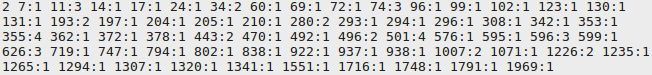
\includegraphics[scale=0.7]{chap5-img/libsvm-example}
	\caption{نمونه‌ای از یک سند منفی در فایل lib-svm}
	\label{chap5-fig1}
\end{figure}


\section{لغت‌نامه‌ی احساس}
\label{chap5sec5}
منظور از لغت‌نامه‌ی احساس یک لغت‌نامه عمومی‌ از پیش ساخته شده است که در آن به ازای هر کلمه برای هر یک از برچسب‌های احساس مثبت، منفی‌ و بی‌طرف وزنی بین ۰ تا ۱ وجود دارد به گونه‌ای که مجموع این مقادیر برای هر کلمه برابر با ۱ است. به عبارت دیگر این لغت‌نامه شامل تعدادی کلمه است که به هیچ دامنه‌ی خاصی‌ وابسته نیستند و برچسب احساسی‌ برای آنها مشخص است. منظور از اینکه این کلمات به هیچ دامنه‌ی خاصی‌ وابسته نیستند و مستقل از دامنه هستند این امر است که به طور مثال در یک موضوع سینمایی کلمه‌ای مثل ''پیچیده`` برای یک فیلمنامه می‌‌تواند احساسی‌ مثبت به همراه داشته باشد، اما همین کلمه در موضوع علمی‌ بار مثبتی به همراه خود ندارد. از این رو بعضی‌ از کلمات از نظر احساسی‌ وابسته به دامنه‌ای هستند که در آن بحث می‌‌شود و در زمینه‌های مختلف می‌‌توانند بار احساسی‌ متفاوتی داشته باشند. اما لغت‌نامه‌ی احساس از کلماتی ساخته می‌‌شود که در تمام دامنه‌‌ها و زمینه‌ها بار احساسی‌ که به همراه خود دارند ثابت است. به طور مثال کلمه ای‌ مانند
``good''
همیشه یک مفهوم مثبت و کلمه‌ای مانند
``bad'' 
 همه‌‌جا یک مفهوم منفی‌ را می‌‌رسانند.

در بخش‌های بعدی در یکی‌ از آزمایش‌های طراحی شده برای مدل پیشنهادی در این پژوهش از یک لغت‌نامه‌ی احساس به نام
MPQA\footnote{Available at http://mpqa.cs.pitt.edu/}
استفاده می‌‌کنیم. این لغت‌نامه احساسی‌ شامل ۴۰۵۳ کلمه است که در مقابل هر لغت یک بردار ۳تایی‌ وجود دارد که عدد اول نشان دهنده‌ی وزن بی‌طرفی، عدد دوم نشان دهنده‌ی وزن مثبت و عدد سوم نشان دهنده‌ی وزن منفی‌ برای آن لغت است. در مجموع در این لغت‌نامه ۱۵۱۱ کلمه‌ی مثبت و ۲۵۴۲ کلمه‌ی منفی‌ وجود دارد. شکل
\ref{chap5-fig2}
نمونه‌ای از کلمات این لغت‌نامه را نشان می‌‌دهد.
\begin{figure}[!b]
	\centering
	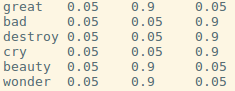
\includegraphics[scale=0.7]{chap5-img/lex-example}
	\caption{نمونه‌ای از لغت‌نامه احساس MPQA شامل ۶ کلمه}
	\label{chap5-fig2}
\end{figure}

\section{جزئیات آموزش مدل پیشنهادی}
\label{chap5sec6}
رويکرد پيشنهادی در اين پژوهش يک مدل احتمالی مولد نظارت شده برای مدل‌سازی همزمان احساس و موضوع در داده‌های متنی می‌باشد که در بخش
\ref{chap4sec5}
به صورت کامل آن را معرفی کردیم. در پایان‌‌نامه برای پياده‌سازی از زبان برنامه‌نويسی پایتون نسخه 2.7 در محيط سيستم عامل لينوکس استفاده شده است. برای پیاده‌سازی ابتدا مدل 
RS
براساس آنچه که در 
\cite{hinton2009replicated}
بيان شده است شبيه‌سازی گرديد، و پس از ارزیابی  و حصول اطمینان از صحت مدل پياده‌سازی شده با بررسی نتايج حاصل از شبيه‌سازی انجام شده با نتايج موجود در 
\cite{hinton2009replicated}
شبيه‌سازی انجام شده را به مدل پيشنهادی در اين پژوهش گسترش داديم.

براساس آنچه که در بخش
\ref{chap5sec4}
بيان کرديم، از پايگاه داده‌ی
MR
در سه حالت مختلف به عنوان داده‌ی ورودی به مدل برای فرآيند آموزش و آزمون استفاده کرديم و نتايج بدست آمده از آزمايشات انجام شده را در بخش‌های بعدی شرح می دهيم. برای آموزش مدل در سه حالات موجود، يعنی با استفاده از ديکشنری های با سايز 2000، 10000 و 24916 ما از الگوريتم 
CD
با مرتبه‌ی ۱ استفاده کرديم. به اين معنی که در مرحله بازسازی داده تنها يک مرحله از اين الگوريتم اجرا شده و جهت گراديان را همان‌طور که آقای 
Hinton
در 
\cite{hinton2002training}
اثبات کرده‌اند تنها با همين يک مرحله تخمين می زنيم. همچنين در هر سه حالت، مدل را به ازای 1000 تکرار\footnote{Epoch, Iteration}
 بر روي کل داده‌هاي آموزش با 
Batch
سايز 1 آموزش داديم و نتايج بدست آمده برای هر حالت را در 2 مرحله، يکی در تکرار ۲۰۰ام و يکی در زمان پايان فرآيند آموزش (تکرار ۱۰۰۰ام) ثبت کرديم. پارامتر ديگری که در آموزش مدل دخيل است تعداد واحدهاي لايه‌ی
Hidden
يا همان تعداد موضوع‌ها است که می توانند متغير باشند. در استفاده از هر 3 ديکشنری، رويکرد پيشنهادی و همچنین مدل 
RS
 را به ازای
$h=\{5,10,15,20,25,30,35,40,45,50,60,70,80,90 \}$
آموزش داديم و نتايج بدست آمده برای حالت‌های مختلف را در ادامه در آزمايش‌های مختلف گزارش می کنيم. برای تمام حالت‌ها از مقدار 
$alfa = 0.001$
برای ضريب يادگيری استفاده کرديم. پارامترهاي 
$W,U,\textbf{a},\textbf{c}$
که به ترتیب وزن بين لايه‌ی 
$Visible$
و
$Hidden$، 
وزن بين لايه‌ی
$Sentiment$
و 
$Hidden$،
باياس لايه‌ی 
$Visible$
و باياس لايه‌ی
$Sentiment$
هستند را با استفاده از مقاديری که به صورت تصادفی از يک توزیع گوسی با ميانگين 0 و واريانس 1 بدست آورديم، مقدار دهی کرديم. همچنين مقدار اوليه‌ی برای باياس لايه‌ی 
$Hidden$
که آن را با 
$\textbf{b}$
نشان داديم را برابر صفر قرار داديم.

\section{مدل‌سازی اسناد و ارزیابی به عنوان یک مدل مولد}
\label{chap5sec7}
در این بخش رویکرد پیشنهادی خودمان را به عنوان یک مدل مولد احتمالاتی با مدل 
RS
در تخمین احتمال برای مشاهده‌ی سندهای پایگاه داده‌های آموزش و تست با استفاده از هر سه لغت‌نامه مورد ارزیابی قرار داده و با تحلیل نتایج بدست آمده نشان می‌‌دهیم که روش پیشنهادی نسبت به روش 
RS
یک روش بهتر در تخمین احتمال برای سندهای دیده نشده و آزمون است. 

برای ارزیابی احتمال محاسبه شده برای مشاهده‌ی اسناد در فرآیند مدل‌سازی مجموعه سند، همان‌طور که در بخش 
\ref{chap5sec1}
گفته شد از یک معیار به نام سرگشتگی استفاده می‌‌شود
\cite{blei2003latent}.
در مباحث مربوط به 
NLP
معیار سرگشتگی پارامتری است که از آن برای مقایسه‌ی مدل‌های احتمالاتی مختلف استفاده می‌شود
\cite{blei2003latent}.
 در فرآیند مدل‌سازی اسناد ما به دنبال تخصیص بالاترین درست‌نمایی به هر سند هستیم و با استفاده از معیار سرگشتگی این مقدار درست‌نمایی 
 محاسبه ‌شده برای هر سند مورد ارزیابی قرار می‌‌گیرد. با توجه به فرمول محاسبه‌ی مقدار سرگشتگی،
\begin{align}
	\centering
	\label{chap5-eq1}
	Perplexity = exp\left( - \dfrac{\sum_{n=1}^{N}\log p(\textbf{v}_n)}{\sum_{n=1}^{N}D_n} \right)
\end{align}
می‌‌توان گفت که مقدار این معیار برابر است با معکوس میانگین درست‌نمایی بدست آماده برای هر سند در مقیاس لگاریتمی به ازای تمام کلمات مجموعه اسناد
\cite{blei2003latent}.
 در یک فرآیند مدل‌سازی و با استفاده از یک مدل احتمالی‌ مناسب مقدار سرگشتی باید به صورت پیوسته و یکنوا کاهش یابد و مدلی که مقدار سرگشتگی کمتری بر روی پایگاه داده آزمون داشته باشد در بحث مدل‌سازی اسناد به عنوان مدل بهتری شناخته می‌‌شود
\cite{blei2003latent}.


در شکل 
\ref{chap5-fig3}
قسمت‌های
\ref{chap5-fig3sub1}
 تا
 \ref{chap5-fig3sub3}
  نمودار تغییرات سرگشتگی در فرآیند آموزش برای مدل پیشنهادی و مدل 
RS
در حالت‌های مخلتف از پایگاه داده‌ی 
MR
نشان داده شده است. همان‌طور که مشاهده می‌‌گردد در هر ۳ نمودار رویکرد پیشنهادی در این پژوهش که یک مدل مشترک احساس موضوع است نسبت به مدل 
RS
که یک رویکرد موضوعی است با کاهش بهتری در مقدار سرگشتگی همراه است. 

برای رسم نمودارهای شکل
\ref{chap5-fig3}
برای هر دو مدل پیشنهادی و مدل
RS
در هر سه‌ حالت مختلف پایگاه داده، در پایان هر مرحله‌ی آموزش مقدار سرگشتگی با استفاده از رابطه‌ی
\ref{chap5-eq1}
برای تمام پایگاه داده‌ی ‌آموزش محاسبه شده و به ازای هر ۱۰ مرحله از آن میانگین گرفته شده است و در انتها با استفاده از این مقادیر نمودارهای حاصل برای مراحل مختلف آموزش رسم گردیده‌اند.

برای هر سه حالت می‌‌توان مشاهده کرد که مقدار افت سرگشتگی در ابتدای فرایند آموزش نسبت به مراحل پایانی با سرعت بیشتری همراه بوده است، به صورتی‌ که از تکرار ۲۰۰ام تا به انتها مقدار سرگشتی با تغییرات آنچنانی همراه نبوده است. مشاهده‌ی این ویژگی‌ در فرایند آموزش موجب گردید که ما هر دو مدل را برای هر سه حالت مختلف پایگاه داده به ازای دو مقدار ۲۰۰ و ۱۰۰۰ چرخه‌، آموزش داده و از نتایج بدست آماده برای تست مدل بر روی پایگاه داده آزمون استفاده کنیم. 

با دقت در نمودار‌های شکل
\ref{chap5-fig3}
می‌توان نتیجه گرفت که با اضافه کردن و در نظر گرفتن احساس و ساخت یک مدل مشترک احتمالاتی مولد، مانند آنچه که در این پژوهش انجام دادیم، در مرحله‌ی آموزش برای مدل‌سازی اسناد مقدار سرگشتگی با افت بیشتری همراه می‌‌شود و در نتیجه روش احتمالاتی مناسب‌تری برای مدل‌سازی اسناد ساخته می‌‌شود.
	\begin{figure}[!t]
		\centering
		\begin{subfigure}{.45\textwidth}
			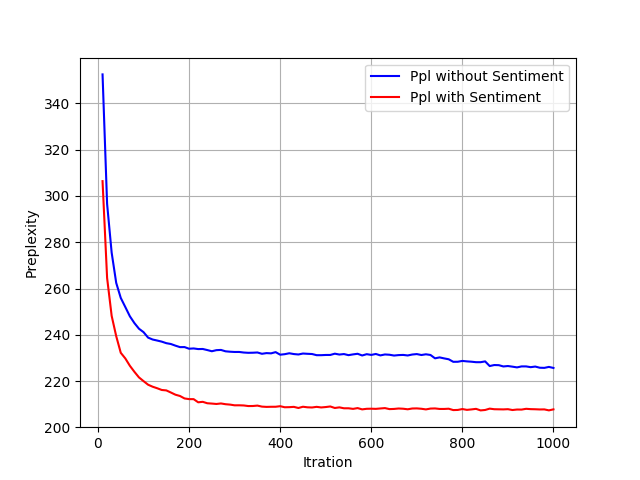
\includegraphics[scale = .4]{chap5-img/ppl_2000}
			\caption{ با استفاده از  لغت‌نامه با اندازه 2000}
			\label{chap5-fig3sub1}
		\end{subfigure}		
		\begin{subfigure}{.45\textwidth}
			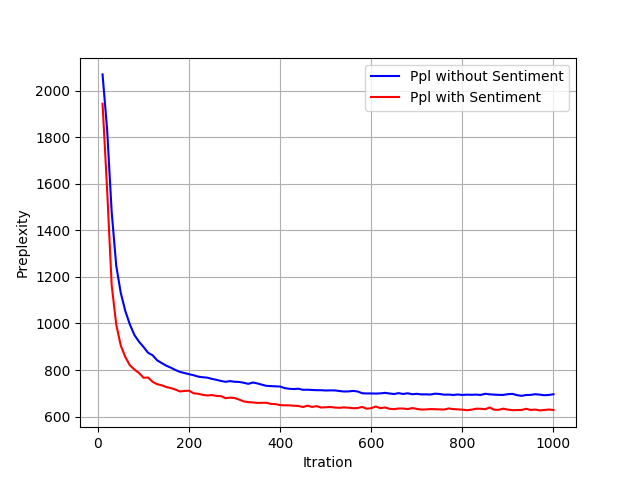
\includegraphics[scale =.4]{chap5-img/ppl_10000}
			\caption{ با استفاده از  لغت‌نامه با اندازه 10000 }
			\label{chap5-fig3sub2}
		\end{subfigure}
		
		\begin{subfigure}{.45\textwidth}
			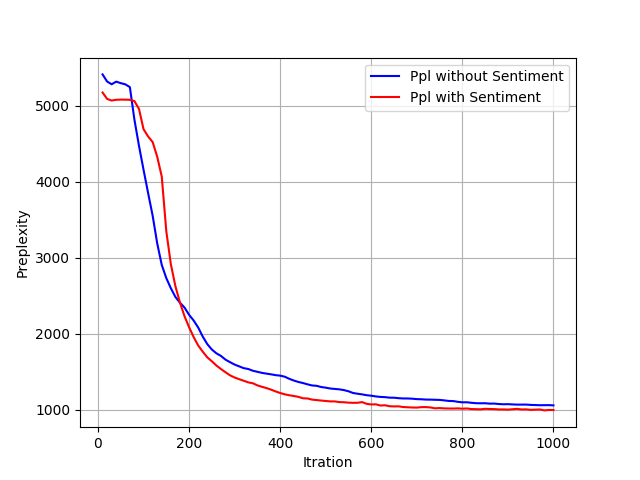
\includegraphics[scale=.4]{chap5-img/ppl_24916}
			\caption{ با استفاده از  لغت‌نامه با اندازه  24916}
			\label{chap5-fig3sub3}
		\end{subfigure}
	\caption{ارزیابی تغییرات سرگشتگی در فرآیند آموزش برروی پایگاه داده‌ی MR  برای مدل پیشنهادی و مدل RS}
	\label{chap5-fig3}
	\end{figure}

مقادير محاسبه شده برای سرگشتگی که در جدول 
\ref{chap5-tb2}
نشان داده شده است نيز دليلی بر اثبات ادعای ما نسبت به بهتر بودن رويکرد پيشنهادی در فرآیند مدل‌سازی به عنوان یک مدل مولد است. در جدول 
\ref{chap5-tb2}
مقدار سرگشتگی برای داده‌هاي تست در پايگاه داده‌ی 
MR
به‌ازای هر 3 ديکشنری مورد استفاده و 2 تکرار 200 و 1000 برای هر کدام محاسبه شده است.

مقادیر بدست آمده برای سرگشتگی در حالت‌های مختلف در جدول
\ref{chap5-tb2}
نشان می‌‌دهد که در حالت‌های استفاده از ۲ لغت‌نامه ۲۰۰۰ و ۱۰۰۰تایی تفاوت مقدار محاسبه شده برای سرگشتگی در مدل هایی که ۱۰۰۰مرحله آموزش دیده‌اند بیشتر است از مدل‌هایی که ۲۰۰ مرحله آموزش دیده‌اند. اما در استفاده از لغت‌نامه‌ی ۲۴۹۱۶تایی شرایط برعکس است و تفاوت در حالتی که هر دو مدل ۲۰۰ مرحله آموزش دیده‌اند بیشتر از زمانی‌ است که مدل‌ها ۱۰۰۰ مرحله آموزش دیده‌اند. در اینجا به نمودارهای شکل
\ref{chap5-fig3}
برمی‌‌گردیم و با مقایسه‌ی نمودار
\ref{chap5-fig3sub3}
با نمودارهای
 \ref{chap5-fig3sub1}
و
 \ref{chap5-fig3sub2}
مشاهده می‌کنیم که نمودار مربوط به حالت ۲۴۹۱۶تایی دارای نوسانات بیشتری نسبت به ۲ حالت دیگر است. به خصوص در  نزدیکی‌ تکرار ۲۰۰ام که مورد بحث ما نیز است نمودار‌های هر ۲ مدل دچار یک تغییر وضعیت نسبت به یکدیگر گشته و شرایط برای آن‌ها بر عکس شده است.

 با توجه به مقادير بدست آمده برای سرگشتگی برروی پایگاه داده‌ی تست برای مدل پیشنهادی در این پژوهش در مقايسه با مدل 
RS
در جدول 
\ref{chap5-tb2},
مشاهده می‌کنيم که در تمامی حالت‌ها رويکرد پيشنهادی مقدار کمتری را برای سرگشتگی محاسبه کرده است. لذا در تایید آنچه که گفتیم نتيجه گرفته 
می‌شود که راهکار پيشنهادی که با اضافه کردن يک لايه برای احساس نيز همراه است منجر به ساخت يک رويکرد احتمالی مناسب‌ برای مدل‌سازی اسناد 
می‌باشد که در مقایسه با مدل 
RS
نتایج بهتری در بحث مدل‌سازی موضوع بدست می‌دهد.

\begin{table}[!t]
	\centering
	\begin{latin}
	\begin{tabular}{|l|c|c|c|c|}
		\hline
		TestSet Type & Num of Docs & Num of Epoch & Ppl without Sentiment & Ppl with Sentiment \\
		\hline
		MR by 2000 & 1000 & 200 & 400.77 & \textbf{393.69 }\\
		\hline
		MR by 2000 & 1000 & 1000 & 423.89 & \textbf{406.74} \\
		\hline
		MR by 10000 & 1000 & 200 & 1553.52 & \textbf{1529.42} \\
		\hline
		MR by 10000 & 1000 & 1000 & 2028.69 & \textbf{1871.57} \\
		\hline
		MR by 24916 & 1000 & 200 & 4237.65 & \textbf{3898.67}\\
		\hline
		MR by 24916 & 1000 & 1000 & 5842.39 & \textbf{5824.97}\\
		\hline
	\end{tabular}
	\end{latin}
	\caption{تخمین سرگشتگی برای پایگاه داده‌ی Review Movie با استفاده از مدل پیشنهادی}
	\label{chap5-tb2}
\end{table}

\section{مجسم‌سازی موضوع‌ها و ارزیابی دقت در محاسبه‌ی آن‌ها}
\label{chap5sec8}
در بخش
\ref{chap5sec5}
یک لغت‌نامه‌ی احساس به نام
MPQA
معرفی‌ کردیم که شامل ۴۰۵۳ کلمه می‌باشد که برچسب احساس برای آن‌ها مشخص شده است. در این بخش با استفاده از این لغت‌نامه‌ی احساس دقت موضوع‌های یاد گرفته شده توسط مدل را از نظر برچسب احساسی مورد ارزیابی قرار می‌‌دهیم.

با توجه به ساختار رویکرد پیشنهادی که در فصل
\ref{chap5}
توضیح داده شد، می‌‌دانیم که هر یک از واحدهای لایه‌ی
$Hidden$
به تمام واحدها چه در لایه‌ی
$Visible$
و چه در لایه‌ی
$Sentiment$
متصل هستند. هر واحد در لایه‌ی
$Sentiment$
برابر با یک برچسب احساسی‌ و هر واحد در لایه‌ی
$Visible$
متناظر با یک کلمه است. از آنجا که در بحث مدل‌سازی موضوعی اسناد متنی، هر موضوع را به صورت یک توزیع احتمالی چند جمله‌ای بر روی تمام کلمات لغت‌نامه معرفی‌ کردیم لذا می‌دانیم که هر واحد در لایه‌ی
$Hidden$
با یک وزن مشخص به تمام کلمات لغت‌نامه در لایه
$Visible$
متصل است. این وزن  برای هر کلمه نشان دهنده‌ی مقدار اهمیت آن کلمه در آن موضوع است.
\begin{table}[!t]
	\centering
	\begin{latin}
		\begin{tabular}{|c|c|c|c|}
			\hline
			& Total Number & Numb of Positive Words & Num of Negative Words \\ \hline
			NG(2000)  &     155      &          100           &          55           \\ \hline
			RCV(10000) &     950      &          447           &          503          \\ \hline
			MR(24916)  &     3114     &          1242          &         1872          \\ \hline
		\end{tabular}
	\end{latin}
	\caption{فراوانی‌های بدست آمده از مقایسه‌ی کلمات مشترک بین لغت‌نامه‌ی احساسی MPQA با سه لغت‌نامه واژگان}
	\label{chap5-tb3}
\end{table}
ایده‌ی ارزیابی مطرح شده در این بخش از آزمایش‌های انجام شده بر روی مدل‌های معروفی‌ در زمینه‌ی مدل‌سازی موضوعی همچون
DocNADE
و
LDA
گرفته شده است. در مدل
DocNADE
که در بخش 
\ref{chap3sec3sub6}
معرفی گردید و یک روش بر پایه‌ی شبکه عصبی است، برای مجسم‌سازی و نشان دادن موضوع‌های یاد گرفته شده توسط مدل از ماتریس وزن بین لایه‌ی
$Hidden$
و بردار کلمات استفاده می‌‌شود. به این صورت که برای هر موضوع وزن‌های تمام کلمات متصل به آن که در واقع تمام کلمات لغت‌نامه هستند مقایسه شده و بطور مثال ۱۰ کلمه‌ای‌ که دارای بیشترین وزن برای هر موضوع هستند به عنوان کلمات متناسب با آن موضوع نشان داده می‌‌شوند. در مدل
LDA
نیز به همین صورت برای نمایش موضوع‌ها عمل می‌‌شود با این تفاوت که در روش
LDA
به جای ماتریس وزن یک ماتریس احتمال داریم و برای هر موضوع بطور مثال ۱۰ کلمه‌ای‌ که بیشترین احتمال در آن موضوع را دارند نشان داده می‌‌شوند.
در این بخش ما نیز از همین ایده کمک گرفته و موضوع‌ها را از نظر برچسب احساسی‌ مورد ارزیابی قرار می‌دهیم.

ابتدا برای هر سه‌ حالت مختلف از پایگاه داده تعداد کلمات مشترک با لغت‌نامه‌ی احساس
MPQA
را محاسبه کردیم. جدول
\ref{chap5-tb3}
نتایج مربوط به این عمل را نشان می‌‌دهد. سپس به ازای هر ۳ حالت از پایگاه داده و ۲ تکرار مختلف برای مرحله‌ی آموزش و همچنین تعداد موضوع‌های مختلف مراحل زیر را به ترتیب انجام دادیم:
\begin{enumerate}
	\item محاسبه‌ی مجموع وزن‌های کلمات مثبت و منفی‌ برای هر موضوع با استفاده از لغت‌نامه‌ی احساس و ماتریس وزن بین لایه‌ی $Visible$ و $Hidden$. 
	\item محاسبه‌ی تفاضل مقادیر حساب شده در مرحله ۱ برای هر موضوع و مرتب کردن مقادیر حاصل به صورت نزولی.
	\item انتخاب ۵ موضوع از ابتدای لیست مرتب (مثبت‌ترین موضوع‌ها) و تخصیص برچسب مثبت به آن‌ها، و ۵ موضوع از انتهای لیست مرتب (منفی‌ترین موضوع‌ها) و تخصیص برچسب منفی‌ به آن‌ها.
	\item مقایسه‌ی برچسب تخصیص داده شده به هر موضوع با وزن‌های متناظر با آن موضوع در اتصال به لایه‌ی
	$Sentiment$
	و محاسبه‌ی دقت.
\end{enumerate}

در مرحله‌ی ۴ام منظور از مقایسه‌ی برچسب تخصیص داده شده به هر موضوع با وزن لایه‌ی
$Sentiment$
به این صورت است که اگر به یک موضوع در مرحله‌ی ۳ برچسب مثبت اختصاص داده شد، باید وزن متناظر با برچسب احساس مثبت برای آن موضوع در لایه‌ی
$Sentiment$
بیشتر از وزن منفی‌ برای همان موضوع باشد و بر عکس.

نمودار‌های
\ref{chap5-fig4sub1}
و
\ref{chap5-fig4sub2}
نتایج حاصل از این ارزیابی را به ازای ۲۰۰ و ۱۰۰۰ مرحله آموزش نشان می‌‌دهند. همان‌طور که مشاهده می‌‌گردد برای هر ۳ حالت مختلف از پایگاه و تعداد موضوع‌های مختلف تفاوتی‌ بین دقت محاسبه شده برای ۲۰۰ و ۱۰۰۰ مرحله‌‌ی آموزش وجود ندارد. اما با دقت در این نمودارها مشاهده می‌‌گردد که با بزرگ شدن اندازه لغت‌نامه دقت مدل در تخصیص برچسب احساسی‌ به موضوع‌ها نیز افزایش می‌‌یابد.

  مقایسه‌ی اطلاعات موجود در جدول
\ref{chap5-tb3}
برای لغت‌نامه‌های مختلف با نمودار‌های شکل
\ref{chap5-fig4}
علت افزایش دقت به ازای افزایش  اندازه لغت‌نامه را برای ما توجیه می‌‌کند. مشاهده می‌‌شود که با بزرگ شدن اندازه‌ی لغت‌نامه تعداد کلمه‌های مشترک بین آن و لغت‌نامه‌ی احساس نیز افزیش پیدا می‌‌کند و این امر سبب می‌گردد که در فرایند آموزش  موضوع‌های مثبت و منفی‌ بیشتر از یکدیگر تفکیک شده و در نتیجه دقت مدل در یادگیری و تخصیص برچسب احساس به موضوع‌ها افزایش پیدا می‌‌کند.
\begin{figure}[!t]
	\centering
	\begin{subfigure}{.46\textwidth}
		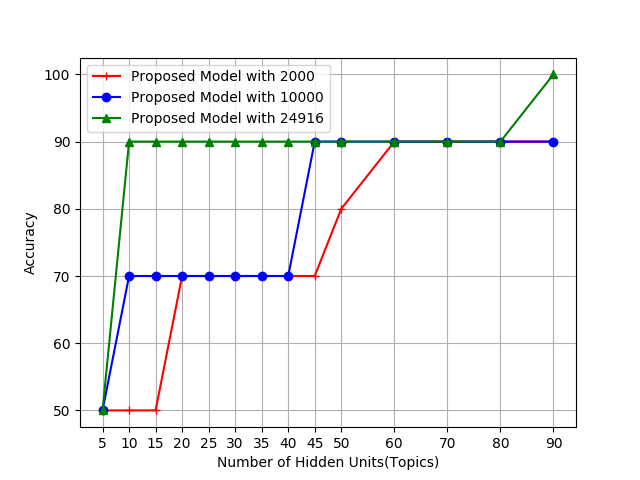
\includegraphics[scale = .48]{chap5-img/v_200}
		\caption{ برای 200 تکرار }
		\label{chap5-fig4sub1}
	\end{subfigure}		
	\begin{subfigure}{.46\textwidth}
		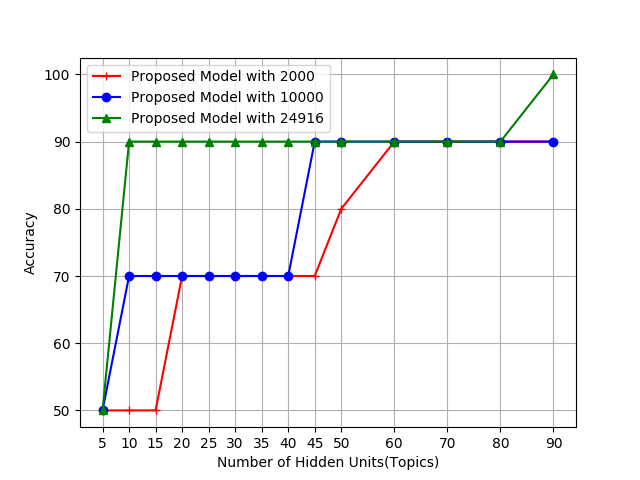
\includegraphics[scale =.48]{chap5-img/v_1000}
		\caption{ برای 1000 تکرار }
		\label{chap5-fig4sub2}
	\end{subfigure}
	\caption{ارزیابی دقت در تخصیص احساس به موضوع‌ها به ۲۰۰ و ۱۰۰۰ مرحله آموزش}
	\label{chap5-fig4}
\end{figure}


\section{طبقه‌بندی احساسی اسناد}
\label{chap5sec9}
در این بخش نتایج حاصل از طبقه‌بندی احساس با استفاده از رویکرد پیشنهادی در این پژوهش را بر روی پایگاه داده‌ی
MR
ارزیابی و گزارش می‌‌کنیم. برای مقایسه‌ی نتایج بدست آمده در بحث طبقه‌بندی احساس با استفاده از مدل پیشنهادی، از یک روش پایه که بر اساس شمارش تعداد کلمات است برای ارزیابی دقت در حالت‌های مختلف بهره می‌‌بریم. همچنین از نتایج بدست آماده برای طبقه‌بندی احساس با استفاده از چند روش معروف نظارت شده مانند ماشین بردار پشتیبان\footnote{Support Vector Machine}
،(SVM)
و دو شبکه عصبی (یک شبکه‌ عصبی با مقادبر اولیه‌ی تصادفی و یک شبکه‌ عصبی با مقادیر اولیه‌ی یادگرفته شده توسط رویکرد پیشنهادی) به منظور ارزیابی پارامترهای یاد گرفته شده توسط مدل استفاده می‌کنیم.

شبکه عصبی‌های استفاده شده در هر دو حالت (مقدار دهی تصادفی و مقدار دهی با پارامترهای یاد گرفته شده توسط مدل پیشنهادی) از دسته شبکه‌های 
MLP\footnote{Multilayer Perceptron}
هستند. در لایه‌ی اول برای هر دو حالت تعداد نورون‌ها برابر با تعداد موضوع‌ها و در لایه‌ی دوم تعداد نورون‌ها برابر با تعداد احساس‌ها هستند. برای هردوی این شبکه‌ها از تابع خطای
Entropy Cross 
استفاده شده است. همچنین در لایه‌ی اول این شبکه‌ها از تابع فعال‌ساز 
tanh
و در لایه‌ی دوم از تابع
Softmax
استفاده شده است.
%
%همچنین علاوه بر یک شبکه عصبی با مقدار دهی‌ اولیه‌ی تصادفی، از یک شبکه عصبی دیگر که مقادیر اولیه در آن با استفاده از پارامترهای یاد گرفته شده توسط مدل پیشنهادی در این پژوهش مقدار دهی‌ می‌‌شوند، برای طبقه‌بندی احساس و ارزیابی نتایج در پایگاه داده‌ی
%MR
%استفاد می‌کنیم که در ادامه نتایج بدست آمده را کامل شرح داده و بررسی‌ می‌‌کنیم.

برای محاسبه‌ی دقت در مدل پایه برای هر سند در پایگاه داده‌ی تست شروع به شمارش کلمات با قطبیت مشخص احساسی‌ می‌‌کنیم. به بیان دیگر برای هر سند تعداد کلمات مثبت و تعداد کلمات منفی را با استفاده از لغت‌نامه‌ی احساس
MPQA
محاسبه می‌کنیم. بعد از محاسبه‌ی تعداد لغات مثبت و منفی‌ برای هر سند اگر این مقدار برای کلمات مثبت در یک سند بیشتر از کلمات منفی‌ بود به سند مورد نظر برچسب مثبت اختصاص دادیم و اگر تعداد کلمات منفی‌ بیشتر بود آن سند را در دسته سندهای منفی‌ دسته‌بندی می‌کنیم.

برای طبقه بندی احساس به کمک رویکرد پیشنهادی در این پژوهش به این صورت عمل می‌کنیم که در ابتد برای هر سند متنی با استفاده از
\begin{align}
	\centering
	\label{chap5-eq2}
	p(h_{j}=1|\textbf{V})=\sigma \left( Db_j + \sum_{k=1}^{K}W_{kj}\hat{v}_k \right)
\end{align}
(این رابطه‌ همان رابطه‌ی \ref{chap4-eq23} است که برای سهولت در اینجا عینا تکرار شده است) مقدار لایه‌ی مخفی متناظر با آن را بدست می آوریم. پس از محاسبه‌ی مقدار لایه‌ی پنهان با استفاده از رابطه‌ی
\ref{chap5-eq2}
مرحله‌ی بعدی محاسبه‌ی لایه‌ی احساس متناظر با سند جاری با استفاده از
\begin{align}
	\centering
	\label{chap5-eq3}
	p(s_{l}=1|\textbf{h})=\dfrac{exp(c_{l}+\sum_{j=1}^{H}U_{lj}h_j)}{\sum_{l=1}^{S}exp(c_{l}+\sum_{j=1}^{H}U_{lj}h_j)}
\end{align}
(این رابطه‌ نیز همان رابطه‌‌ی \ref{chap4-eq30} است)
است. 

همان‌طور که در بخش 
\ref{chap4sec5}
بیان گردید و در رابطه‌ی محاسبه لایه احساس (\ref{chap4-eq30}) مشخص است, چون مقدار این لایه از یک تابع 
$Softmax$
بدست می‌آید لذا به فرم یک توزیع احتمالی است که مجموع درایه‌های آن برابر با 1 است. با بدست آوردن مقدار این لایه‌ی احساس سپس برای تخصیص برچسب به مقادیر این لایه نگاه می‌کنیم و مقدار متناطر با هراحساس که بزرگتر بود برچسب آن سند را برابر با آن احساس انتخاب می کنیم.

نتایج بدست آمده از طبقه‌بندی احساس با استفاده از رویکرد پیشنهادی و مدل پایه برای ۲ حالت مختلف از پایگاه داده‌ در شکل
\ref{chap5-fig5}
نشان داده شده است. برای محاسبه‌ی دقت در طبقه‌بندی احساس با استفاده از مدل پیشنهادی در این پژوهش برای هر ۲ حالت مختلف از پایگاه داده و تعداد موضوع های مختلف از مدل‌هایی که به ازای 1000 تکرار آموزش دیده‌اند استفاده شده است. همچنین برای مقدار دهی اولیه‌ی شبکه عصبی با پارامترهای یاد گرفته شده توسط رویکرد پیشنهادی, از مقادیر بدست آمده برای پارامترها (ماتریس وزن و بایاس) در این حالت (1000 چرخه اموزش) استفاده کردیم.

همانطور که در شکل‌های 
\ref{chap5-fig5sub1}
و
\ref{chap5-fig5sub2}
مشاهده می گردد در هر ۲ حالت دقت طبقه‌بندی برای مدل پیشنهادی با افزایش تعداد موضوع‌ها رو به افزایش بوده است. همچنین در هر ۲ حالت دقت طبقه‌بندی با استفاده از مدل پیشنهادی با افزایش تعداد موضوع‌ها با اختلاف بسيار زیادی از دقت بدست آمده توسط مدل ‌پایه بهتر است. 

%علاوه بر این در حالت استفاده از لغت‌نامه 2000تایی دقت مدل پیشنهادی برای تعداد موضوع های بیشتر از 20 از دقت به دست آمده توسط روش سوم نیز بهتر است. در حالت استفاده لغت‌نامه 2000تایی نیز همچنین برای تعداد موصوع های 80 و 90 دقت به دست آمده توسط مدل پیشنهاد دارای شرایط رقابی با هر 2 مدل شبکه عصبی استفاده شده است, و بااختلاف کمی دیگری پایینتر از انها دارد.  
\begin{figure}[!t]
	\centering
	\begin{subfigure}{.45\textwidth}
		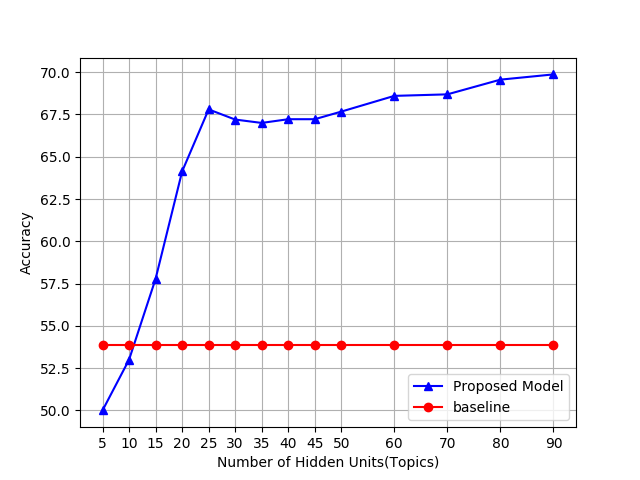
\includegraphics[scale = .4]{chap5-img/sc-a}
		\caption{ با استفاده از  لغت‌نامه با اندازه 2000}
		\label{chap5-fig5sub1}
	\end{subfigure}		
	\begin{subfigure}{.45\textwidth}
		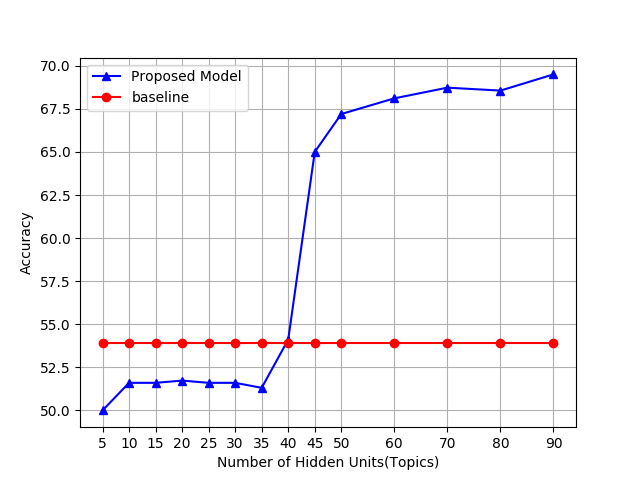
\includegraphics[scale =.4]{chap5-img/sc-b}
		\caption{ با استفاده از  لغت‌نامه با اندازه 10000 }
		\label{chap5-fig5sub2}
	\end{subfigure}
	\caption{طبقه‌بندی احساس در پایگاه داده‌ی MR با استفاده از مدل پیشنهادی و مدل پایه برای موضوع‌های مختلف }
	\label{chap5-fig5}
\end{figure}

با مقایسه‌ي دقت بدست آمده برای طبقه‌بندی احساس به کمک رویکرد پیشنهادی و با استفاده از لغت‌نامه 10000تایی (شکل \ref{chap5-fig5sub2}) با نمودار شکل 
\ref{chap5-fig4sub2}
نتایج جالبی بدست می آید. در نمودار شکل 
\ref{chap5-fig5sub2}
دقت طبقه‌بندی احساس برای روش پیشنهادی در بازه‌ی تعداد موضوع های 40 تا 45 دچار یک جهش بزرگ و افزایش دقت با شیب زیادی می شود. با مقایسه این جهش و بررسی عمیق‌تر نمودار شکل 
\ref{chap5-fig4sub2}
مشاهده می‌شود که ارزیابی دقت در تخصیص برچسب احساس به موضوع‌ها برای لغت‌نامه 10000تایی در بازه 40 تا 45 موضوع با یک افزایش با شیب بسيار زیاد همراه است. لذا نتیجه می شود که هرچه دقت در تخصیص برچسب احساس به موضوع‌ها بالاتر رود, یا به عبارت دیگر هرچه موضوع‌های متمایزتری از نظر احساسی داشته باشیم دقت در بحث طبقه‌بندی احساس نیز بالاتر می‌رود.

شکل 
\ref{chap5-fig6}
دقت نتایج حاصل از طبقه‌بندی احساس با استفاده از ۳ مدل مختلف را نشان می‌دهد. با دقت در نمودارهای شکل
\ref{chap5-fig6}
مشاهده می‌شود که در هر دو حالت مورد نظر برای پایگاه داده, دقت بدست آمده با استفاده از شبکه عصبی با مقدار دهی اولیه توسط پارامترهای یاد گرفته شده در روش پیشنهادی, از دقت بدست آمده توسط هر دو روش دیگر بهتر است.

در حالت استفاده از لغت‌نامه 10000تایی همان‌طور که در شکل 
\ref{chap5-fig6sub2}
مشخص است, تنها زمانی که تعداد موضوع‌ها برابر با 20 و 70 هستند دقت هر دو شبکه عصبی با هم برابر است. در سایر موارد شبکه با مقدار دهی
 اولیه‌ی پارامترها نسبت به هر 3 مدل دیگر نتایج بهتری داشته است. به طور کلی نتیجه می‌شود که در فرآیند طبقه‌بندی احساس، شبکه‌ی عصبی که مقادیر آن توسط پارامترهای یاد گرفته شده توسط مدل پیشنهادی مقدار دهی اولیه می‌شوند از عملکرد بهتری نسبت به سایر مدل‌ها برخوردار است.
\begin{figure}[!t]
	\centering
	\begin{subfigure}{.45\textwidth}
		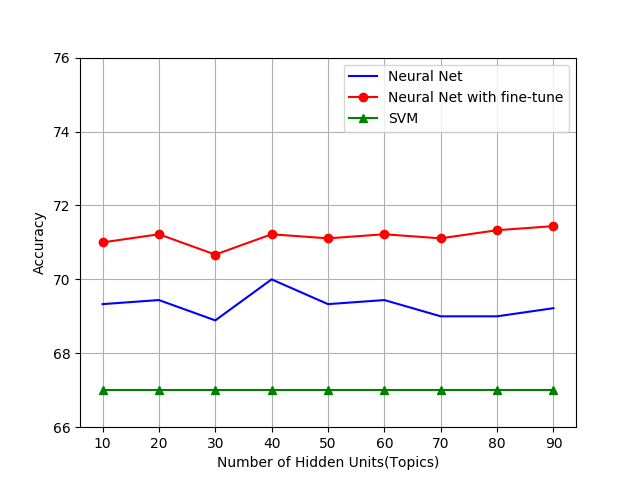
\includegraphics[scale = .4]{chap5-img/sc-c}
		\caption{ با استفاده از  لغت‌نامه با اندازه 2000}
		\label{chap5-fig6sub1}
	\end{subfigure}		
	\begin{subfigure}{.45\textwidth}
		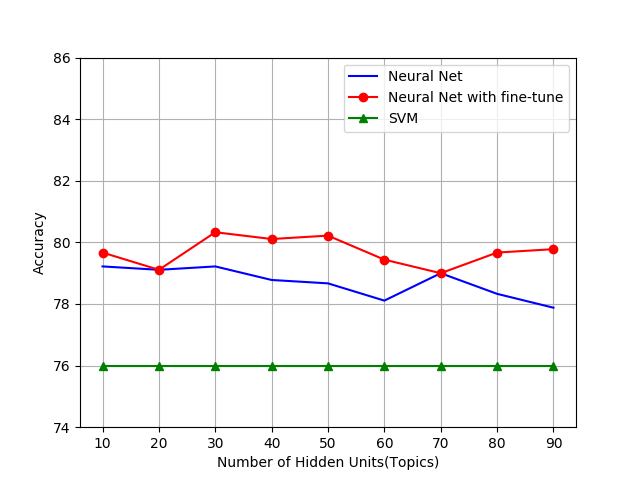
\includegraphics[scale =.4]{chap5-img/sc-d}
		\caption{ با استفاده از  لغت‌نامه با اندازه 10000 }
		\label{chap5-fig6sub2}
	\end{subfigure}
	\caption{طبقه‌بندی احساس در پایگاه داده‌ی MR با استفاده از مدل‌های شبکه عصبی با مقدار دهی اولیه برای وزن‌ها و بایاس‌ها، شبکه عصبی و SVM }
	\label{chap5-fig6}
\end{figure}

\section{بازیابی اطلاعات}
\label{chap5sec10}
با توجه به اینکه رویکرد پیشنهادی در  این پژوهش یک روش مولد برای مدل‌سازی همزمان احساس و موضوع است، لذا گام نخست برای ارزیابی این مدل در بحث بازیابی اطلاعات استفاده از پایگاه داده‌ای است که علاوه بر برچسب احساس برای اسناد، دارای برچسب موضوع برای هر سند نیز باشد. با توجه به عدم وجود یک چنین پایگاه داده‌ای، در این پژوهش ۲ پایگاه داده که همزمان شامل برچسب احساس و برچسب موضوع هستند ساخته شده است.

اولین پایگاه داده‌ی احساس‌-موضوع ساخته شده در این قسمت با تخصیص برچسب احساس به دیتاست
20NG
ساخته می‌‌شود. در بخش
\ref{chap5sec11}
پایگاه داده‌ی
20NG
را معرفی‌ کردیم. همان‌طور که بیان شد
20NG
یک پایگاه داده‌ی معیار در بخش مدل‌سازی موضوعی است. اسناد موجود در
20NG
شامل ۲۰ گروه مختلف می‌‌شوند که هر یک از گروه‌ها در مورد یک موضوع خاص، مانند سیاسی، ورزشی، علمی‌ و غیره هستند. برای اضافه کردن احساس به این مجموعه، مانند آنچه که در بخش
\ref{chap5sec9}
برای بدست آوردن دقت مدل پایه برای طبقه‌بندی احساس گفته شد، برای هر سند به شمارش تعداد کلمات با قطبیت مشخص احساسی‌ با استفاده از 
لغت‌نامه‌ی احساس
MPQA
کردیم. سپس برای هر سند اگر تعداد کلمات مثبت بیشتر بود به آن سند برچسب مثبت اختصاص دادیم و برعکس. در فایل
lib-svm
که برای این پایگاه داده ساخته می‌‌شود، برای هر سند عدد اول نشان دهنده‌ی احساس (۱ مثبت، ۲ منفی‌) و عدد دوم (عددی از ۱ تا ۲۰) نشان 
دهند‌ه‌ی موضوع مانند:\\ 
\begin{latin}
	SentimentLabel \ TopicLabel \ <ID:Count> \ <ID:Count> \ <ID:Count> \ ... 
\end{latin} 
برای آن سند است.

پایگاه داده‌ی دومی‌ که برای ارزیابی رویکرد پیشنهادی در این پژوهش در بحث بازیابی اطلاعات ساخته می‌‌شود، از ترکیب چند دیتاست بدست می‌‌آید. 
پایگاه داده‌های
MR
و
MDS
در بخش‌های
\ref{chap5sec3}
و
\ref{chap5sec12}
به ترتیب معرفی‌ شدند. هر کدام از این ۵ پایگاه داده 
(
MDS
 شامل ۴ بخش مختلف با ۲۰۰۰ سند در هر بخش است) 
تنها شامل برچسب احساس هستند. می‌‌توان هر کدام از این مجموعه اسناد را به صورت یک موضوع خاص در نظر گرفت. به عبارت دیگر با کنار هم قرار دادن این پایگاه داده‌ها می‌‌توان یک پایگاه داده بزرگتر ایجاد کرد. این دیتاست جدید ساخته شده شامل ۱۰۰۰۰ سند است که ۵۰۰۰تا از آن‌ها دارای برچسب مثبت و ۵۰۰۰تای دیگر دارای برچسب منفی‌ هستند. همچنین این پایگاه داده‌ی جدید شامل ۵ موضوع مختلف که بازبینی‌ فیلم، کتاب، دی‌وی‌دی، وسایل آشپزخانه و وسایل الکترونیکی‌ هستند،می‌‌شود. پس اتمام مرحله‌ی پیش‌پردازش هر کدام از این اسناد با استفاده از لغت‌نامه پایگاه داد‌ه‌ی
20NG
(۲۰۰۰ کلمه) به فایل
libsvm
تبدیل شدند. از ۱۰۰۰۰ سند نتیجه که با ترکیب این ۵ پایگاه داده بدست می‌‌آید، ۷۵۰۰ سند برای مجموعه آموزش با توزیع مساوی از نظر برچسب احساس (۳۷۵۰ سند مثبت و ۳۷۵۰ سند منفی‌) و موضوع ( ۱۵۰۰ سند از هر موضوع که ۷۵۰تای آن مثبت و ۷۵۰تای دیگر منفی‌ هستند) انتخاب شدند و مابقی 
مجموعه‌ی تست را که شامل ۲۵۰۰ سند (۵۰۰ سند از هر موضوع که ۲۵۰تای آن مثبت و ۲۵۰تای آن منفی‌ هستند) است، تشکیل می‌‌دهند. این پایگاه داده‌ی ساخته شده را به اختصار 
MRMDS
نام‌گذاری می‌کنیم.

\begin{figure}[!b]
	\centering
	\begin{subfigure}{.45\textwidth}
		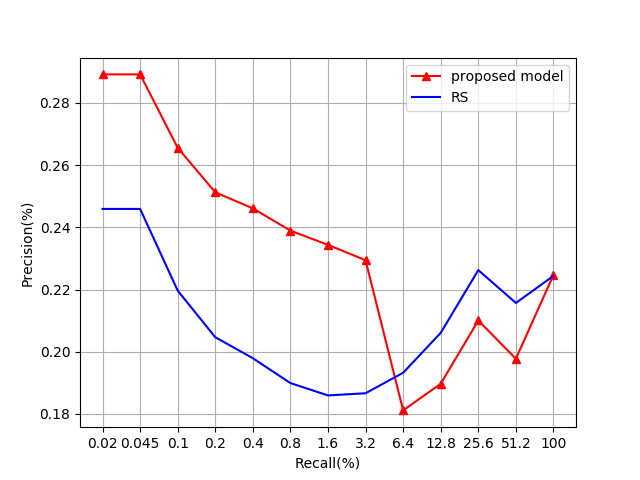
\includegraphics[scale = .4]{chap5-img/ir-1}
		\caption{پایگاه داده‌ی Groups News 20}
		\label{chap5-fig7sub1}
	\end{subfigure}		
	\begin{subfigure}{.45\textwidth}
		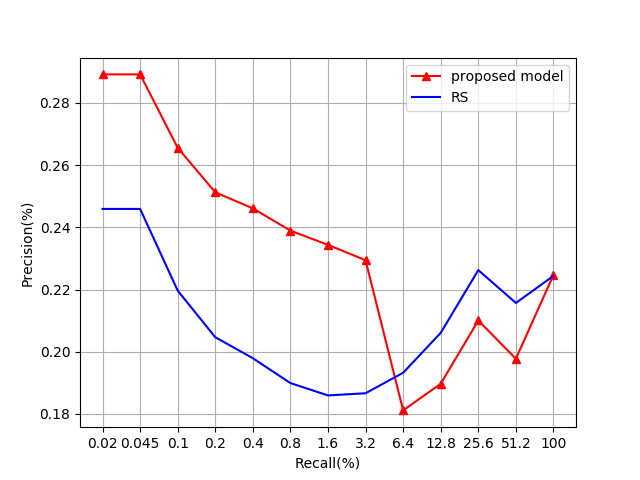
\includegraphics[scale =.4]{chap5-img/ir-2}
		\caption{ پایکاه داده‌ی MRMDS}
		\label{chap5-fig7sub2}
	\end{subfigure}
	\caption{بازیابی اطلاعات با استفاده ۲ پایگاه داده‌ی Groups News 20 و MRMDS برای رویکرد پیشنهادی و مدل RS}
	\label{chap5-fig7}
\end{figure}
پس از ساخت پایگاه داده‌های مورد نیاز، به ارزیابی بازیابی اطلاعات برای رویکرد پیشنهادی در این پژوهش در مقایسه با مدل
RS
که در بخش
\ref{chap3sec3sub5}
معرفی‌ شد می‌‌پردازیم. هدف از این ارزیابی مشاهده تاثیر در نظر گرفتن احساس برای بازیابی اطلاعات با استفاده از ساختار پیشنهادی در این پژوهش است. برای ارزیابی مورد نظر از نمودار صحت در برابر فراخوانی\footnote{Precision vs Recall}
استفاده می‌‌کنیم. این نمودار به عنوان معروف‌ترین معیار در بحث ارزیابی بازیابی اطلاعات و مقایسه‌ی روش‌های مختلف در این زمینه شناخته می‌‌شود. برای رسم این نمودار از مقادیر مختلف صحت و فراخوانی که توسط هر مدل بدست می‌‌آیند در برابر یکدیگر استفاده می‌‌شود. روابط
\begin{align}
	\centering
	\label{chap5-eq4}
	recall = \dfrac{TP}{C^+}
\end{align}
و
\begin{align}
	\centering
	\label{chap5-eq5}
	precision = \dfrac{TP}{R^+}
\end{align}
شیوه‌ی محاسبه‌ی مقادیر فراخوانی و صحت را نشان می‌‌دهند. منظور از
TP
در هر دو رابطه‌ی
\ref{chap5-eq4}
و
\ref{chap5-eq5}
مثبت‌های واقعی‌\footnote{True Positive}
 است که آن را برابر با تعداد اسنادی تعریف می‌‌کنیم که برچسب موضوعی برای آن‌ها همان برچسب مورد نظر ما است و مدل نیز آن‌ها را 
درست تشخیص داده است.
$C^+$
در رابطه‌ی
\ref{chap5-eq4}
نشان دهنده‌ی تعداد کل سندهای موجود با برچسب مورد نظر ما در پایگاه داده است و
$R^+$
نشان دهنده‌ی تعداد اسنادی است که مدل آن‌ها را برای ما هماهنگ با برچسب مورد نظر ما تشخیص داده است.


نمودار‌های شکل
\ref{chap5-fig5}
نتایج حاصل از ارزیابی بازیابی اطلاعات برای رویکرد پیشنهادی در این پژوهش و همچنین مدل
RS
را نشان می‌‌دهند. همان‌طور که مشاهده می‌‌شود برای هر ۲ نمودار شکل
\ref{chap5-fig5}
بخصوص نمودار
\ref{chap5-fig5sub1}
روش پیشنهادی در این پژوهش عملکرد بهتری را در مقایسه با مدل
RS
در بحث بازیابی اطلاعات داشته است. برای محاسبه مقادیر صحت و فراخوانی و رسم نمودار‌های شکل
\ref{chap5-fig5}
به این صورت عمل شده است که، ابتدا بر روی هر کدام از پایگاه داده‌ها مدل پیشنهادی در این پژوهش بدون در نظر گرفتن برچسب موضوع و تنها با برچسب احساس و لایه‌ی مخفی با اندازه 50، و همچنین روش
RS
بدون در نظر گرفتن برچسب‌های احساس و موضوع و لابه‌ی مخفی با اندازه 50 به ازای ۵۰۰ تکرار آموزش داده شده‌اند. در مرحله‌ی بعدی برای تک‌تک سند‌های مجموعه‌ی تست در هر پایگاه داده مقدار شباهت کسینوسی\footnote{Cosine Similarity}
هر سند با تمام اسناد پایگاه داده‌ی آموزش محاسبه شده و مقادیر دقت و فراخوانی به دست آمده‌اند. در ادامه مقادیر بدست آمده برای صحت برای کل پایگاه داده‌ی تست میانگین گرفته می‌‌شوند و نمودار‌های
\ref{chap5-fig5sub1}
و
\ref{chap5-fig5sub2}
رسم می‌‌شوند.

\section{نتیجه‌گیری}
در این فصل رویکرد پیشنهادی در این پژوهش که یک مدل مولد احتمالاتی نظارت شده برای مدل‌سازی مشترک موضوع و احساس در داده‌های متنی است مورد ارزیابی‌های مختلفی‌ قرار گرفت.  برای انجام این ارزیابی‌ها از چند پایگاه داده معروف در بحث مدل‌سازی موضوع و احساس استفاده گردید که هر کدام از آن‌ها در بخش‌های متفاوتی معرفی‌ و به تفصیل شرح داده شدند. همچنین در این فصل یک لغت‌نامه‌ی احساس معرفی‌ شد و با ساختار آن آشنا شدیم. در فصل بعدی نتجه‌گیری نهایی از پژوهش و پیشنهادات آینده مطرح می‌گردند.

 	\chapter{نتیجه‌گیری و پیشنهادات}
\thispagestyle{empty}
\section{نتیجه‌گیری}
پیشرفت گسترده و چشمگیر در دنیای امروز که از آن به عنوان عصر ارتباطات و تکنولوژی یاد می‌کنیم منجر به تولید حجم بسيار زیادی از شکل‌های مختلف داده شده است. داده‌های تصویری, صوتی, متنی و غیره که هر روز مقدار آن‌ها بخصوص در بستر اینترنت رو به افزایش است. استفاده از این حجم عظیم از انواع مختلف داده که با سرعتی بسيار زیاد در حال افزایش نیز هستند نیاز به رویکردها و ساختارهایی دارد که توانایی تطبیق با این نرخ رشد را داشته باشند. مدل‌هایی که با پردازش اتوماتیک و خودکار این داده‌ها بتوانند از آن‌ها اطلاعات مفید و مورد نظر را استخراج کنند. بدون شک این حجم گسترده از شکل‌های مختلف داده حاوی اطلاعات سودمند بسياری هستند که با استخراج آن‌ها می‌توان در کاربردهای گوناگون بهره‌های مناسبی از آن‌ها بدست آورد. 

داده‌های متنی نیز در این میان از سهم بالایی برخوردار هستند. این شکل از داده هر روز در شبکه‌های اجتماعی, سایت‌های خرید و فروش, گروه‌های بحث و تبادل نظر, مجلات برخط و غیره در حال تولید و افزایش هستند. با تحلیل این داده‌ها, پردازش واستخراج اطلاعات از آن‌ها می‌توان به نتایج جالبی از قبیل مهم‌ترین موارد مطرح شده در شبکه‌های اجتماعی,احساس کلی کاربران و افراد جامعه در موارد خاص, بیشترین و مهم‌ترین موضوع‌های مطرح شده در مجلات و برخظ و غیره بدست آورد. هدف ما در این پایان‌‌نامه نیز در همین راستا قرار داشت. ما به دنبال ساختاری مناسب و رویکردی جدید برای مدل‌سازی اسناد متنی واستخراج اتوماتیک اطلاعات, بخصوص اطلاعات مفهومی واحساس موجود در اسناد بودیم.

با توجه به مطالب بیان شده, هدف کلی در این پایان‌‌نامه ساخت مدلی بر پایه‌ی شبکه‌های عصبی برای مدل‌سازی مشترک موضوع واحساس در داده‌های متنی است. در فصل سوم این پایان‌‌نامه با روش‌های پیشین موجود در این زمینه آشنا شدیم. همان‌طور که گفته شد ساختارهای موجود در اکثر موارد تنها به مدل‌سازی موضوع و یا تشخیص احساس در پایگاه داده می‌پردازند. بررسی‌های انجام شده نشان داد که در زمینه‌ی مدل‌سازی مشترک موضوع واحساس تنها دو مدل
ASUM (\ref{chap3sec4sub2})
و 
JST (\ref{chap3sec4sub1})
وجود دارند که با آن‌ها نیز به صورت کامل آشنا شدیم. گسترش شبکه‌های عصبی در سال‌های اخیر و استفاده‌ی فراوان از آن‌ها در بخش‌ها و زمینه‌های مختلف, همچنین عدم وجود ساختاری بر پایه‌ی شبکه‌های عصبی در زمینه‌ی مدل‌سازی مشترک احساس و موضوع به همراه کمبودها و کاستی‌های مدل‌های موجود در این زمینه دلایل اصلی نگارند‌ه‌ی این پایان‌‌نامه برای ساخت رویکردی جدید در این زمینه و انجام این پایان‌‌نامه بوده است.

در این پایان‌‌نامه یک رویکرد نظارت شده با استفاده از شبکه‌های عصبی برای مدل‌سازی مشترک موضوع واحساس در داده‌های متنی پیشنهاد شد. این ساختار که در دسته روش‌های احتمالاتی مولد دسته‌بندی می‌گردد با گسترش مدل معروف ماشین بلتزمن محدود ایجاد می‌شود. در این رویکرد پیشنهادی یک لایه‌ی جدید با ماهیت توزیع احتمالاتی چندجمله‌ای به مدل اضافه شده و منجر به یادگیری ویژگی‌های بهتر و متمایز کننده‌تری برای هر سند در لایه‌ی مخفی
می‌شود. همان‌طور که در فصل 
\ref{chap5}
بیان گردید برای یادگیری و آموزش در این مدل از الگوریتم واگرایی مقابله استفاده می‌کنیم که یک روش تقریبی برای تخمین گرادیان است.

برای ارزیابی مدل پیشنهادی از پایگاه داده‌های بازبینی فیلم
،(MR)
 20 گروه خبری 
(20NG)
 و احساس چند دامنه 
(MDS)
 که همگی از پایگاه داده‌های شاخص در بحث مدل‌سازی موضوع و احساس  در داده‌های متنی هستند، استفاده کردیم. با استفاده از یک معيار معروف برای ارزیابی مدل‌های مولد به نام سرگشتگی, رویکرد پیشنهادی در این پایان‌‌نامه را در فرآیند مدل‌سازی اسناد متنی ارزیابی کردیم. با توجه به نتایج بدست آمده در این بخش ادعا می‌کنیم که با در نظر گرفتن احساس موجود در اسناد و ایجاد ساختاری مانند آنچه که ما در این پایان‌‌نامه انجام دادیم, یک مدل مولد بهتر برای مدل‌سازی اسناد ساخته می‌شود. همچنین با استفاده از پایگاه داده 
MR
 دقت رویکرد پیشنهادی را در زمینه‌های طبقه‌بندی احساس و ارزیابی موضوع‌های یاد گرفته شده مورد برررسی قرار دادیم و نتایج مربوط به آن را در بخش‌های
\ref{chap5sec8}
و
\ref{chap5sec9}
گزارش کردیم. در بخش
\ref{chap5sec10}
نیز رویکرد پیشنهادی در این پایان‌‌نامه را در بحث بازیابی اطلاعات در مقایسه با مدل
RS
مورد ارزیابی قرار دادیم. با انجام آزمایش بر روی ۲ پایگاه داده‌‌ی مختلف و مقایسه‌ی نتایج مشاهده گردید که روش پیشنهادی نتایج بهتری را در بحث بازیابی اطلاعات بر روی داده‌های متنی دارد و از دقت بالاتری در این زمینه برخوردار است.

علی‌رغم اینکه در زمینه‌ی طبقه‌بندی احساس نتایج بدست آمده توسط رویکرد پیشنهادی در مقایسه با روش‌های موجود در بعضی حالت‌ها رقابتی است, اما مدل پیشنهادی در این پایان‌‌نامه از نقاط قوت دیگری همچون نمایش موضوع‌های یاد گرفته شده و دقت بهتر در فرآیند مدل‌سازی به عنوان یک مدل مولد برخوردار است که آن را از دیگر روش‌های موجود در این زمینه متمایز می‌کند.


\section{پیشنهاد‌ها}
مدل پیشنهادی در این پایان‌‌نامه
(فصل 
\ref{chap5})
از یک ساختار نظارت شده برای مدل‌سازی استفاده می‌کند. با توجه به اینکه حجم عظیمی از داده‌های موجود در بستر اینترنت داده‌های بدون برچسب هستند, لذا ساخت مدل‌های نیمه نظارتی, نظارت شده‌ی ضعیف و بدون نظارت به صورت قابل ملاحظه‌ای کاربردی و حائز اهمیت هستند. ساخت این دسته از مدل‌ها با گسترش رویکرد پیشنهادی از جمله مهم‌ترین کارهای پیش‌ رو در این پایان‌نامه است. 

%در روش پیشنهادی نسبت اندازه لایه‌ی 
%$Sentiment$
%اندازه لایه‌ی
%$Visible$
%و
%$Hidden$
%مقدار بسیار کوچکی است که این امر می‌تواند موجب پایین آمدن کیفیت آموزش و نتایج نهایی گردد. می‌توان با تغییر رابطه‌ی محاسبه‌ی انرژی و به تبعیت از آن روابط مربوط به آپدیت پارامترها به گونه‌ای که مشکل عدم تعادل در اندازه‌ی لایه‌ها برطرف شود، به مقدار مناسب‌تری برای پارامترهای در پی فرایند آموزش رسید و همچنین نتایج بهتری در بخش عملی از مدل بدست آورد.

پیشنهاد دیگری که در این قسمت برای کارهای آینده می‌تواند مطرح گردد استفاده از اید‌ه‌ی ماشین بلتزمن محدود شرطی و ارائه‌ی مدل‌های عمیق\footnote{Deep Model}
برای استخراج ویژگی‌های سطح بالاتر است. در ساختار پیشنهادی در این پایان‌‌نامه به ازای هر سند یک بردار ویژگی به نام لایه‌ي مخفی
از آن استخراج می کنیم. پس ازاستخراج این بردار ویژگی از هر سند می‌توان خود این بردار را به عنوان یک داده‌ی ورودی برای یک شبکه عصبی 
RBM
در نظر گرفت و مجددا از آن ویژگی استخراج کرد. این ساختار منجر به یاد گرفتن ویژگی‌های متمایزتری برای هر داده‌ی ورودی می‌گردد.

رویکرد پیشنهادی در این پایان‌‌نامه بر اساس کیسه‌ی کلمات عمل می‌کند. در استفاده از کیسه‌ی کلمات ساختار جملات و داده‌های ورودی از بین می‌روند و تنها تعداد تکرار کلمه‌ها مهم هستند. اما داده‌های متنی از سری داده‌های دنباله‌دار هستند و ترتیب در آن‌ها اهمیت دارد. لذا با در نظر گرفتن وابستگی کلمه‌ها در کنار یکدیگر و ترتیب آن‌ها می‌توان ویژگی‌های متمایز کننده‌تری از متن استخراج کرد. با توجه به اینکه در اکثر مواردی که بحث داده‌های دارای توالی مطرح می‌شود از شبکه‌های عصبی بازگشتی\footnote{Recurrent Neural Networks}
برای پياده‌سازی استفاده می‌گردد, لذا پیشنهاد می‌کنیم در این حالت نیز از این شبکه‌ها استفاده شود.

%\section{دسترسی به پیاده‌سازی‌های و پایگاه داده‌ها}
%همان‌طور که پیش از این بیان گردید، برای پياده‌سازی در این پایان‌‌نامه از زبان برنامه‌نویسی پایتون 2.7 در محیط سیستم عامل لینوکس استفاده شده است. فایل‌های مربوط به پياده‌سازی‌های انجام شده بر روی سایت گیت‌هاب بارگذاری شده\footnote{https://github.com/Masoud-Fatemi/final.git}
%و قابل دسترسی و دانلود هستند. همچنین فایل‌های مربوط به پایگاه داده‌های استفاده شده در این پایان‌‌نامه در یک فایل فشرده روی 
%DropBox
% قابل دریافت هستند\footnote{https://www.dropbox.com/s/yxgos056qgx92sq/DataSets.zip?dl=0}.
%

 	\pagestyle{empty}
 	\resetlatinfont 	
 	\begin{LTRitems}
 		\addcontentsline{toc}{section}{مراجع}
 		\onehalfspacing
 		\bibliographystyle{IEEEtran}
 		%\bibliographystyle{plain}
 		%{plain}%{chicago-fa}%{plainnat-fa}%
 		\bibliography{IEEEabrv,refs} 		
 	\end{LTRitems} 	
 	
\addcontentsline{toc}{section}{چکیده انگلیسی}
\thispagestyle{empty}

\begin{latin}
	\begin{center}
		
		{\Huge \textbf{Extension of Restricted Boltzman Machine for Joint Sentiment Topic Modeling in Text Data}}
		
		\vspace{1cm}
		
		{\LARGE{Masoud Fatemi}}
		
		\vspace{0.2cm}
		
		{\small m.fatemi@ec.iut.ac.ir}
		
		\vspace{0.5cm}
		
		June , 2017
		
		\vspace{0.5cm}
		
		Department of Electrical and Computer Engineering
		
		\vspace{0.2cm}
		
		Isfahan University of Technology, Isfahan 84156-83111, Iran
		
		\vspace{0.2cm}
		
		Degree: M.Sc. \hspace*{3cm} Language: Farsi
		
		\vspace{1cm}
		
		{\small\textbf{Supervisor: Prof. Mehran Safayani (safayani@cc.iut.ac.ir)}}\\
		{\small\textbf{Advisor: Prof. Abdolreza Mirzaei (mirzaei@cc.iut.ac.ir)}}
	\end{center}
	~\vfill
	
	
	
	\noindent\textbf{Abstract}
	
	\begin{small}
		\baselineskip=0.6cm
Recently by the development of the internet and web, different types of social media such as web blogs became an immense source of text data. Through the processing of these data, not only is it possible to discover practical information about different topics, but it is also feasible to know about individual’s opinions and gain a thorough understanding of the society sentiment. Therefore, having models which can automatically extract the subjective information from the documents would be efficient and helpful. Topic modeling procedures in addition data mining and also sentiment analysis are the most topics which considered in the natural language processing and text mining fields. Most of the existed models in these fields are based on the statistical methods and Bayesian networks so that there is no method for sentiment-topic modeling based on neural networks. Besides, the majority of existed frameworks have some constraint and difficulties such as computational complexity. This Thesis proposes a new structure for joint sentiment-topic modeling based on Restricted Boltzman Machine which is a type of neural networks. By altering the structure of Restricted Boltzman Machine plus appending a layer to it which is analogous to text data sentiment, feasibly we can suggest a generative structure for joint sentiment topic modeling based on neutral network. Suggested method is a supervised procedure which is trained by the Contrastive Divergence algorithm. The new attached layer in suggested model is a layer with the multinomial probability distribution quiddity which can be used in text data sentiment classification or any other supervised application. The proposed model is compared to existed models After implementing on document modeling as a generative model, sentiment classification and information retrieval the corresponding results have been reported thoroughly. It is observed that in the sentiment classification experiment the suggested model has a better accuracy on average of 11\% in comparison with baseline model. Additionally, in the process of information retrieval on 20 news group‘s dataset, the proposed model by considering sentiment has an average of 9\% enhanced function rather than the case in which sentiment is disregarded. 
	
		
	\end{small}
	
	\vspace{0.5 cm}
	
	
	\noindent \textbf{Key Words}: Topic Model, Sentiment Analysis, Neural Networks, Restricted Boltzman Machine, Probabilistic Model, Contrastive Divergence Algorithm
\end{latin}

	
 \end{document}